\documentclass[a4paper]{book}
\usepackage{a4wide}
\usepackage{makeidx}
\usepackage{fancyhdr}
\usepackage{graphicx}
\usepackage{multicol}
\usepackage{float}
\usepackage{textcomp}
\usepackage{alltt}
\usepackage{times}
\usepackage{ifpdf}
\ifpdf
\usepackage[pdftex,
            pagebackref=true,
            colorlinks=true,
            linkcolor=blue,
            unicode
           ]{hyperref}
\else
\usepackage[ps2pdf,
            pagebackref=true,
            colorlinks=true,
            linkcolor=blue,
            unicode
           ]{hyperref}
\usepackage{pspicture}
\fi
\usepackage[utf8]{inputenc}
\usepackage{doxygen}
\makeindex
\setcounter{tocdepth}{3}
\renewcommand{\footrulewidth}{0.4pt}
\begin{document}
\begin{titlepage}
\vspace*{7cm}
\begin{center}
{\Large Reference Manual}\\
\vspace*{1cm}
{\large Generated by Doxygen 1.5.8}\\
\vspace*{0.5cm}
{\small Sun May 17 21:05:28 2009}\\
\end{center}
\end{titlepage}
\clearemptydoublepage
\pagenumbering{roman}
\tableofcontents
\clearemptydoublepage
\pagenumbering{arabic}
\chapter{Class Index}
\section{Class Hierarchy}
This inheritance list is sorted roughly, but not completely, alphabetically:\begin{CompactList}
\item \contentsline{section}{kern::kern}{\pageref{classkern_1_1kern}}{}
\begin{CompactList}
\item \contentsline{section}{kern::bias}{\pageref{classkern_1_1bias}}{}
\item \contentsline{section}{kern::component}{\pageref{classkern_1_1component}}{}
\begin{CompactList}
\item \contentsline{section}{kern::cmpnd}{\pageref{classkern_1_1cmpnd}}{}
\end{CompactList}
\item \contentsline{section}{kern::lin}{\pageref{classkern_1_1lin}}{}
\item \contentsline{section}{kern::rbf}{\pageref{classkern_1_1rbf}}{}
\item \contentsline{section}{kern::white}{\pageref{classkern_1_1white}}{}
\end{CompactList}
\item \contentsline{section}{kerndox::kern}{\pageref{classkerndox_1_1kern}}{}
\begin{CompactList}
\item \contentsline{section}{kerndox::bias}{\pageref{classkerndox_1_1bias}}{}
\item \contentsline{section}{kerndox::component}{\pageref{classkerndox_1_1component}}{}
\begin{CompactList}
\item \contentsline{section}{kerndox::cmpnd}{\pageref{classkerndox_1_1cmpnd}}{}
\end{CompactList}
\item \contentsline{section}{kerndox::lin}{\pageref{classkerndox_1_1lin}}{}
\item \contentsline{section}{kerndox::rbf}{\pageref{classkerndox_1_1rbf}}{}
\item \contentsline{section}{kerndox::white}{\pageref{classkerndox_1_1white}}{}
\end{CompactList}
\end{CompactList}

\chapter{Class Index}
\section{Class List}
Here are the classes, structs, unions and interfaces with brief descriptions:\begin{CompactList}
\item\contentsline{section}{\hyperlink{classkern_1_1bias}{kern::bias} }{\pageref{classkern_1_1bias}}{}
\item\contentsline{section}{\hyperlink{classkerndox_1_1bias}{kerndox::bias} }{\pageref{classkerndox_1_1bias}}{}
\item\contentsline{section}{\hyperlink{classkerndox_1_1cmpnd}{kerndox::cmpnd} }{\pageref{classkerndox_1_1cmpnd}}{}
\item\contentsline{section}{\hyperlink{classkern_1_1cmpnd}{kern::cmpnd} }{\pageref{classkern_1_1cmpnd}}{}
\item\contentsline{section}{\hyperlink{classkerndox_1_1component}{kerndox::component} }{\pageref{classkerndox_1_1component}}{}
\item\contentsline{section}{\hyperlink{classkern_1_1component}{kern::component} }{\pageref{classkern_1_1component}}{}
\item\contentsline{section}{\hyperlink{classkern_1_1kern}{kern::kern} }{\pageref{classkern_1_1kern}}{}
\item\contentsline{section}{\hyperlink{classkerndox_1_1kern}{kerndox::kern} }{\pageref{classkerndox_1_1kern}}{}
\item\contentsline{section}{\hyperlink{classkern_1_1lin}{kern::lin} }{\pageref{classkern_1_1lin}}{}
\item\contentsline{section}{\hyperlink{classkerndox_1_1lin}{kerndox::lin} }{\pageref{classkerndox_1_1lin}}{}
\item\contentsline{section}{\hyperlink{classkern_1_1rbf}{kern::rbf} }{\pageref{classkern_1_1rbf}}{}
\item\contentsline{section}{\hyperlink{classkerndox_1_1rbf}{kerndox::rbf} }{\pageref{classkerndox_1_1rbf}}{}
\item\contentsline{section}{\hyperlink{classkern_1_1white}{kern::white} }{\pageref{classkern_1_1white}}{}
\item\contentsline{section}{\hyperlink{classkerndox_1_1white}{kerndox::white} }{\pageref{classkerndox_1_1white}}{}
\end{CompactList}

\chapter{Class Documentation}
\hypertarget{classkern_1_1bias}{
\section{kern::bias Class Reference}
\label{classkern_1_1bias}\index{kern::bias@{kern::bias}}
}
Inheritance diagram for kern::bias::\begin{figure}[H]
\begin{center}
\leavevmode
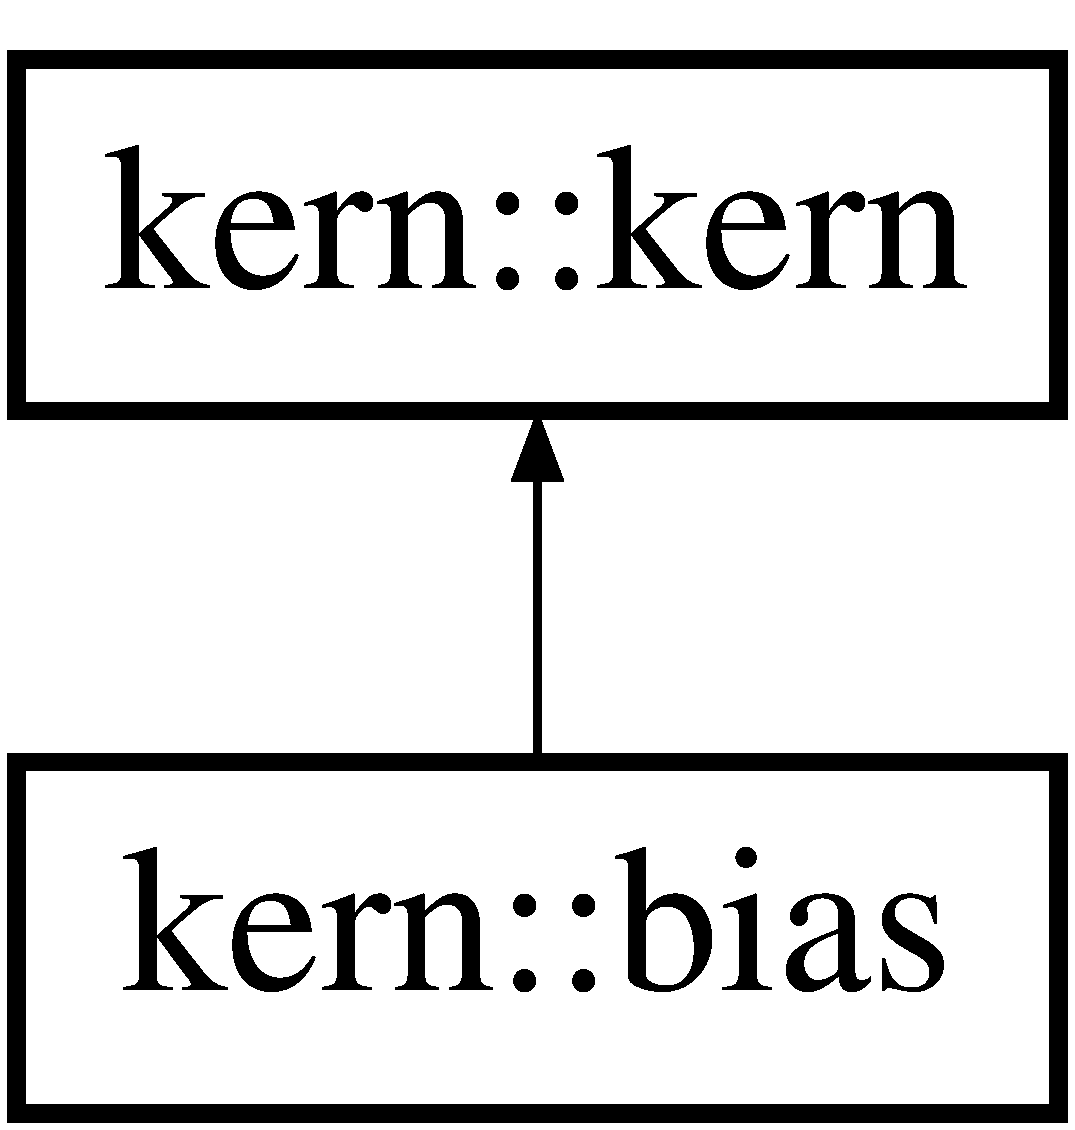
\includegraphics[height=2cm]{classkern_1_1bias}
\end{center}
\end{figure}
\subsection*{Public Member Functions}
\begin{CompactItemize}
\item 
\hypertarget{classkern_1_1bias_0019fb71ede6f8d6d8a4e4738c8e7565}{
def \textbf{\_\-\_\-init\_\-\_\-}}
\label{classkern_1_1bias_0019fb71ede6f8d6d8a4e4738c8e7565}

\item 
def \hyperlink{classkern_1_1bias_39576d2e5f8f5fa8ffab2de6597bb295}{paramInit}
\item 
def \hyperlink{classkern_1_1bias_eac30cc736065001ecadc1d5053a9170}{compute}
\item 
def \hyperlink{classkern_1_1bias_9cb634c409600f556ee51e1205986859}{diagCompute}
\item 
def \hyperlink{classkern_1_1bias_ccc65546498307dfbc396d3612b826fe}{diagGradX}
\item 
def \hyperlink{classkern_1_1bias_06a7443d3cdcb0c7b433b452cb84f357}{diagGradient}
\item 
def \hyperlink{classkern_1_1bias_c1b8e81b9b0942aa0dbe393f8069f0d6}{display}
\item 
def \hyperlink{classkern_1_1bias_9a869f2def84ada0aee7698139c31ea2}{expandParam}
\item 
def \hyperlink{classkern_1_1bias_f9b0c3a62a227ad4480e501e3ebb10f4}{extractParam}
\item 
\hypertarget{classkern_1_1bias_6a387587db971d0ca177d86fdd274717}{
def \textbf{extractParamNames}}
\label{classkern_1_1bias_6a387587db971d0ca177d86fdd274717}

\item 
def \hyperlink{classkern_1_1bias_f27d4ed48a7df56e86609c27dd1ab430}{gradX}
\item 
def \hyperlink{classkern_1_1bias_7a982606235bcbcee2cbd4b1d1cabef7}{gradient}
\end{CompactItemize}
\subsection*{Public Attributes}
\begin{CompactItemize}
\item 
\hypertarget{classkern_1_1bias_b01b8a7df8c614c1c1827a55b78c876d}{
\textbf{type}}
\label{classkern_1_1bias_b01b8a7df8c614c1c1827a55b78c876d}

\item 
\hypertarget{classkern_1_1bias_f367a38c7014cb11f9d71a800e719263}{
\textbf{variance}}
\label{classkern_1_1bias_f367a38c7014cb11f9d71a800e719263}

\item 
\hypertarget{classkern_1_1bias_c5c9e016f6149ac0bbe2c906364eda12}{
\textbf{nParams}}
\label{classkern_1_1bias_c5c9e016f6149ac0bbe2c906364eda12}

\item 
\hypertarget{classkern_1_1bias_3e4b086138955cb5eb4b29ddef844dc8}{
\textbf{stationary}}
\label{classkern_1_1bias_3e4b086138955cb5eb4b29ddef844dc8}

\end{CompactItemize}


\subsection{Detailed Description}


\footnotesize\begin{verbatim}% The white noise kernel arises from assuming independent Gaussian
% noise for each point in the function. The variance of the noise is
% given by the kern.variance parameter.
% 
% This kernel is not intended to be used independently, it is provided
% so that it may be combined with other kernels in a compound kernel.\end{verbatim}
\normalsize
 

\subsection{Member Function Documentation}
\hypertarget{classkern_1_1bias_eac30cc736065001ecadc1d5053a9170}{
\index{kern::bias@{kern::bias}!compute@{compute}}
\index{compute@{compute}!kern::bias@{kern::bias}}
\subsubsection[{compute}]{\setlength{\rightskip}{0pt plus 5cm}def kern::bias::compute ( {\em self}, \/   {\em x}, \/   {\em x2} = {\tt None})}}
\label{classkern_1_1bias_eac30cc736065001ecadc1d5053a9170}




\footnotesize\begin{verbatim}% BIASKERNCOMPUTE Compute the BIAS kernel given the parameters and X.
% FORMAT
% DESC computes the kernel parameters for the bias noise
% kernel given inputs associated with rows and columns.
% ARG kern : the kernel structure for which the matrix is computed.
% ARG x : the input matrix associated with the rows of the kernel.
% ARG x2 : the inpute matrix associated with the columns of the kernel.
% RETURN k : the kernel matrix computed at the given points.
%
% FORMAT
% DESC computes the kernel matrix for the bias noise
% kernel given a design matrix of inputs.
% ARG kern : the kernel structure for which the matrix is computed.
% ARG x : input data matrix in the form of a design matrix.
% RETURN k : the kernel matrix computed at the given points.
%
% SEEALSO : biasKernParamInit, kernCompute, create, biasKernDiagCompute
%
% COPYRIGHT : Neil D. Lawrence, 2004, 2005, 2006, 2009

\end{verbatim}
\normalsize
 

Reimplemented from \hyperlink{classkern_1_1kern}{kern::kern}.\hypertarget{classkern_1_1bias_9cb634c409600f556ee51e1205986859}{
\index{kern::bias@{kern::bias}!diagCompute@{diagCompute}}
\index{diagCompute@{diagCompute}!kern::bias@{kern::bias}}
\subsubsection[{diagCompute}]{\setlength{\rightskip}{0pt plus 5cm}def kern::bias::diagCompute ( {\em self}, \/   {\em x})}}
\label{classkern_1_1bias_9cb634c409600f556ee51e1205986859}




\footnotesize\begin{verbatim}% BIASKERNDIAGCOMPUTE Compute diagonal of BIAS kernel.
% FORMAT
% DESC computes the diagonal of the kernel matrix for the bias noise kernel given a design matrix of inputs.
% ARG kern : the kernel structure for which the matrix is computed.
% ARG x : input data matrix in the form of a design matrix.
% RETURN k : a vector containing the diagonal of the kernel matrix
% computed at the given points.
%
% SEEALSO : biasKernParamInit, kernDiagCompute, create, biasKernCompute
%
% COPYRIGHT : Neil D. Lawrence, 2004, 2005, 2006, 2009

\end{verbatim}
\normalsize
 

Reimplemented from \hyperlink{classkern_1_1kern}{kern::kern}.\hypertarget{classkern_1_1bias_06a7443d3cdcb0c7b433b452cb84f357}{
\index{kern::bias@{kern::bias}!diagGradient@{diagGradient}}
\index{diagGradient@{diagGradient}!kern::bias@{kern::bias}}
\subsubsection[{diagGradient}]{\setlength{\rightskip}{0pt plus 5cm}def kern::bias::diagGradient ( {\em self}, \/   {\em X}, \/   {\em covDiag})}}
\label{classkern_1_1bias_06a7443d3cdcb0c7b433b452cb84f357}




\footnotesize\begin{verbatim}% BIASKERNDIAGGRADIENT Compute the gradient of the BIAS kernel's diagonal wrt parameters.
% FORMAT
% DESC computes the gradient of functions of the diagonal of the
% bias noise kernel matrix with respect to the parameters of the kernel. The
% parameters' gradients are returned in the order given by the
% biasKernExtractParam command.
% ARG kern : the kernel structure for which the gradients are
% computed.
% ARG x : the input data for which the gradient is being computed.
% ARG factors : partial derivatives of the function of interest with
% respect to the diagonal elements of the kernel.
% RETURN g : gradients of the relevant function with respect to each
% of the parameters. Ordering should match the ordering given in
% biasKernExtractParam.
%
% SEEALSO : biasKernParamInit, kernDiagGradient, biasKernExtractParam, biasKernGradient
%
% COPYRIGHT : Neil D. Lawrence, 2004, 2005, 2006, 2009

\end{verbatim}
\normalsize
 

Reimplemented from \hyperlink{classkern_1_1kern}{kern::kern}.\hypertarget{classkern_1_1bias_ccc65546498307dfbc396d3612b826fe}{
\index{kern::bias@{kern::bias}!diagGradX@{diagGradX}}
\index{diagGradX@{diagGradX}!kern::bias@{kern::bias}}
\subsubsection[{diagGradX}]{\setlength{\rightskip}{0pt plus 5cm}def kern::bias::diagGradX ( {\em self}, \/   {\em X})}}
\label{classkern_1_1bias_ccc65546498307dfbc396d3612b826fe}




\footnotesize\begin{verbatim}% BIASKERNDIAGGRADX Gradient of BIAS kernel's diagonal with respect to X.
% FORMAT
% DESC computes the gradient of the diagonal of the bias noise kernel matrix with
% respect to the elements of the design matrix given in X.
% ARG kern : the kernel structure for which gradients are being computed.
% ARG X : the input data in the form of a design matrix.
% RETURN gX : the gradients of the diagonal with respect to each element
% of X. The returned matrix has the same dimensions as X.
%
% SEEALSO : biasKernParamInit, kernDiagGradX, biaskernGradX
%
% COPYRIGHT : Neil D. Lawrence, 2004, 2005, 2006, 2009

\end{verbatim}
\normalsize
 

Reimplemented from \hyperlink{classkern_1_1kern}{kern::kern}.\hypertarget{classkern_1_1bias_c1b8e81b9b0942aa0dbe393f8069f0d6}{
\index{kern::bias@{kern::bias}!display@{display}}
\index{display@{display}!kern::bias@{kern::bias}}
\subsubsection[{display}]{\setlength{\rightskip}{0pt plus 5cm}def kern::bias::display ( {\em self}, \/   {\em numSpaces} = {\tt 0})}}
\label{classkern_1_1bias_c1b8e81b9b0942aa0dbe393f8069f0d6}




\footnotesize\begin{verbatim}% BIASKERNDISPLAY Display parameters of the BIAS kernel.
% FORMAT
% DESC displays the parameters of the bias noise
% kernel and the kernel type to the console.
% ARG kern : the kernel to display.
%
% FORMAT does the same as above, but indents the display according
% to the amount specified.
% ARG kern : the kernel to display.
% ARG spacing : how many spaces to indent the display of the kernel by.
%
% SEEALSO : biasKernParamInit, modelDisplay, kernDisplay
%
% COPYRIGHT : Neil D. Lawrence, 2004, 2005, 2006, 2009

\end{verbatim}
\normalsize
 

Reimplemented from \hyperlink{classkern_1_1kern}{kern::kern}.\hypertarget{classkern_1_1bias_9a869f2def84ada0aee7698139c31ea2}{
\index{kern::bias@{kern::bias}!expandParam@{expandParam}}
\index{expandParam@{expandParam}!kern::bias@{kern::bias}}
\subsubsection[{expandParam}]{\setlength{\rightskip}{0pt plus 5cm}def kern::bias::expandParam ( {\em self}, \/   {\em params})}}
\label{classkern_1_1bias_9a869f2def84ada0aee7698139c31ea2}




\footnotesize\begin{verbatim}% BIASKERNEXPANDPARAM Create kernel structure from BIAS kernel's parameters.
% FORMAT
% DESC returns a bias noise kernel structure filled with the
% parameters in the given vector. This is used as a helper function to
% enable parameters to be optimised in, for example, the NETLAB
% optimisation functions.
% ARG kern : the kernel structure in which the parameters are to be
% placed.
% ARG param : vector of parameters which are to be placed in the
% kernel structure.
% RETURN kern : kernel structure with the given parameters in the
% relevant locations.
%
% SEEALSO : biasKernParamInit, biasKernExtractParam, kernExpandParam
%
% COPYRIGHT : Neil D. Lawrence, 2004, 2005, 2006

\end{verbatim}
\normalsize
 \hypertarget{classkern_1_1bias_f9b0c3a62a227ad4480e501e3ebb10f4}{
\index{kern::bias@{kern::bias}!extractParam@{extractParam}}
\index{extractParam@{extractParam}!kern::bias@{kern::bias}}
\subsubsection[{extractParam}]{\setlength{\rightskip}{0pt plus 5cm}def kern::bias::extractParam ( {\em self})}}
\label{classkern_1_1bias_f9b0c3a62a227ad4480e501e3ebb10f4}




\footnotesize\begin{verbatim}% BIASKERNEXTRACTPARAM Extract parameters from the BIAS kernel structure.
% FORMAT
% DESC Extract parameters from the bias noise kernel structure into a
% vector of parameters for optimisation.
% ARG kern : the kernel structure containing the parameters to be
% extracted.
% RETURN param : vector of parameters extracted from the kernel. If
% the field 'transforms' is not empty in the kernel matrix, the
% parameters will be transformed before optimisation (for example
% positive only parameters could be logged before being returned).
%
% FORMAT
% DESC Extract parameters and parameter names from the bias noise
% kernel structure.
% ARG kern : the kernel structure containing the parameters to be
% extracted.
% RETURN param : vector of parameters extracted from the kernel. If
% the field 'transforms' is not empty in the kernel matrix, the
% parameters will be transformed before optimisation (for example
% positive only parameters could be logged before being returned).
% RETURN names : cell array of strings giving paramter names.
%
% SEEALSO biasKernParamInit, biasKernExpandParam, kernExtractParam, scg, conjgrad
%
% COPYRIGHT : Neil D. Lawrence, 2004, 2005, 2006

\end{verbatim}
\normalsize
 \hypertarget{classkern_1_1bias_7a982606235bcbcee2cbd4b1d1cabef7}{
\index{kern::bias@{kern::bias}!gradient@{gradient}}
\index{gradient@{gradient}!kern::bias@{kern::bias}}
\subsubsection[{gradient}]{\setlength{\rightskip}{0pt plus 5cm}def kern::bias::gradient ( {\em self}, \/   {\em X}, \/   {\em X2} = {\tt None}, \/   {\em covGrad} = {\tt None})}}
\label{classkern_1_1bias_7a982606235bcbcee2cbd4b1d1cabef7}




\footnotesize\begin{verbatim}% BIASKERNGRADIENT Gradient of BIAS kernel's parameters.
% FORMAT
% DESC computes the gradient of functions with respect to the
% bias noise
% kernel's parameters. As well as the kernel structure and the
% input positions, the user provides a matrix PARTIAL which gives
% the partial derivatives of the function with respect to the
% relevant elements of the kernel matrix. 
% ARG kern : the kernel structure for which the gradients are being
% computed.
% ARG x : the input locations for which the gradients are being
% computed. 
% ARG partial : matrix of partial derivatives of the function of
% interest with respect to the kernel matrix. The argument takes
% the form of a square matrix of dimension  numData, where numData is
% the number of rows in X.
% RETURN g : gradients of the function of interest with respect to
% the kernel parameters. The ordering of the vector should match
% that provided by the function kernExtractParam.
%
% FORMAT
% DESC computes the derivatives as above, but input locations are
% now provided in two matrices associated with rows and columns of
% the kernel matrix. 
% ARG kern : the kernel structure for which the gradients are being
% computed.
% ARG x1 : the input locations associated with the rows of the
% kernel matrix.
% ARG x2 : the input locations associated with the columns of the
% kernel matrix.
% ARG partial : matrix of partial derivatives of the function of
% interest with respect to the kernel matrix. The matrix should
% have the same number of rows as X1 and the same number of columns
% as X2 has rows.
% RETURN g : gradients of the function of interest with respect to
% the kernel parameters.
%
% SEEALSO biasKernParamInit, kernGradient, biasKernDiagGradient, kernGradX
%
% COPYRIGHT : Neil D. Lawrence, 2004, 2005, 2006, 2009

\end{verbatim}
\normalsize
 

Reimplemented from \hyperlink{classkern_1_1kern}{kern::kern}.\hypertarget{classkern_1_1bias_f27d4ed48a7df56e86609c27dd1ab430}{
\index{kern::bias@{kern::bias}!gradX@{gradX}}
\index{gradX@{gradX}!kern::bias@{kern::bias}}
\subsubsection[{gradX}]{\setlength{\rightskip}{0pt plus 5cm}def kern::bias::gradX ( {\em self}, \/   {\em X}, \/   {\em X2} = {\tt None})}}
\label{classkern_1_1bias_f27d4ed48a7df56e86609c27dd1ab430}




\footnotesize\begin{verbatim}% BIASKERNGRADX Gradient of BIAS kernel with respect to input locations.
% FORMAT
% DESC computes the gradident of the bias noise
% kernel with respect to the input positions where both the row
% positions and column positions are provided separately.
% ARG kern : kernel structure for which gradients are being
% computed.
% ARG x1 : row locations against which gradients are being computed.
% ARG x2 : column locations against which gradients are being computed.
% RETURN g : the returned gradients. The gradients are returned in
% a matrix which is numData2 x numInputs x numData1. Where numData1 is
% the number of data points in X1, numData2 is the number of data
% points in X2 and numInputs is the number of input
% dimensions in X.
%
% SEEALSO biasKernParamInit, kernGradX, biasKernDiagGradX
%
% COPYRIGHT : Neil D. Lawrence, 2004, 2005, 2006

\end{verbatim}
\normalsize
 

Reimplemented from \hyperlink{classkern_1_1kern}{kern::kern}.\hypertarget{classkern_1_1bias_39576d2e5f8f5fa8ffab2de6597bb295}{
\index{kern::bias@{kern::bias}!paramInit@{paramInit}}
\index{paramInit@{paramInit}!kern::bias@{kern::bias}}
\subsubsection[{paramInit}]{\setlength{\rightskip}{0pt plus 5cm}def kern::bias::paramInit ( {\em self}, \/   {\em inDim} = {\tt None}, \/   {\em X} = {\tt None})}}
\label{classkern_1_1bias_39576d2e5f8f5fa8ffab2de6597bb295}




\footnotesize\begin{verbatim}% BIASKERNPARAMINIT BIAS kernel parameter initialisation.
%
% SEEALSO : cmpndKernParamInit
%
% FORMAT
% DESC initialises the bias noise
%  kernel structure with some default parameters.
% ARG kern : the kernel structure which requires initialisation.
% RETURN kern : the kernel structure with the default parameters placed in.
%
% SEEALSO : create, kernParamInit
%
% COPYRIGHT : Neil D. Lawrence, 2004, 2005, 2006, 2009

\end{verbatim}
\normalsize
 

The documentation for this class was generated from the following file:\begin{CompactItemize}
\item 
kern.py\end{CompactItemize}

\hypertarget{classkerndox_1_1bias}{
\section{kerndox::bias Class Reference}
\label{classkerndox_1_1bias}\index{kerndox::bias@{kerndox::bias}}
}
Inheritance diagram for kerndox::bias::\begin{figure}[H]
\begin{center}
\leavevmode
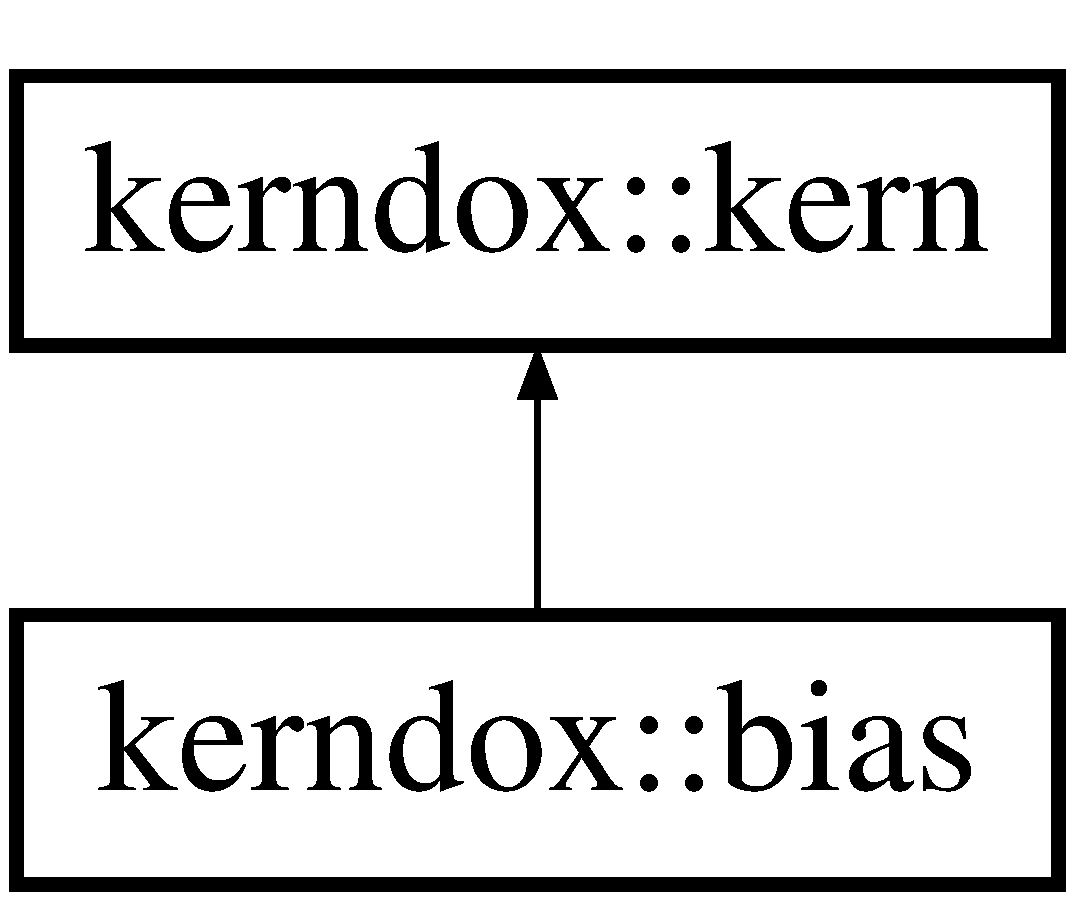
\includegraphics[height=2cm]{classkerndox_1_1bias}
\end{center}
\end{figure}
\subsection*{Public Member Functions}
\begin{CompactItemize}
\item 
\hypertarget{classkerndox_1_1bias_6b49a4ecfb36a98c6fc5485d7b56e5d6}{
def \textbf{\_\-\_\-init\_\-\_\-}}
\label{classkerndox_1_1bias_6b49a4ecfb36a98c6fc5485d7b56e5d6}

\item 
def \hyperlink{classkerndox_1_1bias_7fa82a25834e1b5253409e86e2dbba02}{paramInit}
\item 
def \hyperlink{classkerndox_1_1bias_378a35b6a66d06ae6275e7bb72496012}{compute}
\item 
def \hyperlink{classkerndox_1_1bias_2a8cdcea02456f6083c608daa0e8449a}{diagCompute}
\item 
def \hyperlink{classkerndox_1_1bias_3f9d5af55498317e3fb015d274efabbf}{diagGradX}
\item 
def \hyperlink{classkerndox_1_1bias_66d203c06ed866e4f1c9a09e13a9a142}{diagGradient}
\item 
def \hyperlink{classkerndox_1_1bias_93abbcf30b93880cdddc8b3d5e5b6cb6}{display}
\item 
def \hyperlink{classkerndox_1_1bias_a884620ce9dd942d85f25f3de4703a31}{expandParam}
\item 
def \hyperlink{classkerndox_1_1bias_af12f2b815114cc8b2203236ff333364}{extractParam}
\item 
\hypertarget{classkerndox_1_1bias_7356296b48570bcc12fa549d2ccf8293}{
def \textbf{extractParamNames}}
\label{classkerndox_1_1bias_7356296b48570bcc12fa549d2ccf8293}

\item 
def \hyperlink{classkerndox_1_1bias_d19a0539d91a6cf8deda239b18bd7163}{gradX}
\item 
def \hyperlink{classkerndox_1_1bias_f7f4db511633014f8acf332a7ef0fa78}{gradient}
\end{CompactItemize}
\subsection*{Public Attributes}
\begin{CompactItemize}
\item 
\hypertarget{classkerndox_1_1bias_1b9e89a9037b0a6989d415b05ab1e850}{
\textbf{type}}
\label{classkerndox_1_1bias_1b9e89a9037b0a6989d415b05ab1e850}

\item 
\hypertarget{classkerndox_1_1bias_3a1192ad6f99f2067521d78c03b8c88e}{
\textbf{variance}}
\label{classkerndox_1_1bias_3a1192ad6f99f2067521d78c03b8c88e}

\item 
\hypertarget{classkerndox_1_1bias_9fddce667a3e211e3491028d0f856b5b}{
\textbf{nParams}}
\label{classkerndox_1_1bias_9fddce667a3e211e3491028d0f856b5b}

\item 
\hypertarget{classkerndox_1_1bias_a8cc3c35b1b54709709098a9e0ee27ce}{
\textbf{stationary}}
\label{classkerndox_1_1bias_a8cc3c35b1b54709709098a9e0ee27ce}

\end{CompactItemize}


\subsection{Detailed Description}


\footnotesize\begin{verbatim}The white noise kernel arises from assuming independent Gaussian
noise for each point in the function. The variance of the noise is
given by the kern.variance parameter.

This kernel is not intended to be used independently, it is provided
so that it may be combined with other kernels in a compound kernel.\end{verbatim}
\normalsize
 

\subsection{Member Function Documentation}
\hypertarget{classkerndox_1_1bias_378a35b6a66d06ae6275e7bb72496012}{
\index{kerndox::bias@{kerndox::bias}!compute@{compute}}
\index{compute@{compute}!kerndox::bias@{kerndox::bias}}
\subsubsection[{compute}]{\setlength{\rightskip}{0pt plus 5cm}def kerndox::bias::compute ( {\em self}, \/   {\em x}, \/   {\em x2} = {\tt None})}}
\label{classkerndox_1_1bias_378a35b6a66d06ae6275e7bb72496012}




\footnotesize\begin{verbatim}BIASKERNCOMPUTE Compute the BIAS kernel given the parameters and X.
FORMAT
DESC computes the kernel parameters for the bias noise
kernel given inputs associated with rows and columns.
\param kern : the kernel structure for which the matrix is computed.
\param x : the input matrix associated with the rows of the kernel.
\param x2 : the inpute matrix associated with the columns of the kernel.
\return  k : the kernel matrix computed at the given points.
%
FORMAT
DESC computes the kernel matrix for the bias noise
kernel given a design matrix of inputs.
\param kern : the kernel structure for which the matrix is computed.
\param x : input data matrix in the form of a design matrix.
\return  k : the kernel matrix computed at the given points.
%
SEEALSO : biasKernParamInit, kernCompute, create, biasKernDiagCompute
%
COPYRIGHT : Neil D. Lawrence, 2004, 2005, 2006, 2009

\end{verbatim}
\normalsize
 

Reimplemented from \hyperlink{classkerndox_1_1kern}{kerndox::kern}.\hypertarget{classkerndox_1_1bias_2a8cdcea02456f6083c608daa0e8449a}{
\index{kerndox::bias@{kerndox::bias}!diagCompute@{diagCompute}}
\index{diagCompute@{diagCompute}!kerndox::bias@{kerndox::bias}}
\subsubsection[{diagCompute}]{\setlength{\rightskip}{0pt plus 5cm}def kerndox::bias::diagCompute ( {\em self}, \/   {\em x})}}
\label{classkerndox_1_1bias_2a8cdcea02456f6083c608daa0e8449a}




\footnotesize\begin{verbatim}BIASKERNDIAGCOMPUTE Compute diagonal of BIAS kernel.
FORMAT
DESC computes the diagonal of the kernel matrix for the bias noise kernel given a design matrix of inputs.
\param kern : the kernel structure for which the matrix is computed.
\param x : input data matrix in the form of a design matrix.
\return  k : a vector containing the diagonal of the kernel matrix
computed at the given points.
%
SEEALSO : biasKernParamInit, kernDiagCompute, create, biasKernCompute
%
COPYRIGHT : Neil D. Lawrence, 2004, 2005, 2006, 2009

\end{verbatim}
\normalsize
 

Reimplemented from \hyperlink{classkerndox_1_1kern}{kerndox::kern}.\hypertarget{classkerndox_1_1bias_66d203c06ed866e4f1c9a09e13a9a142}{
\index{kerndox::bias@{kerndox::bias}!diagGradient@{diagGradient}}
\index{diagGradient@{diagGradient}!kerndox::bias@{kerndox::bias}}
\subsubsection[{diagGradient}]{\setlength{\rightskip}{0pt plus 5cm}def kerndox::bias::diagGradient ( {\em self}, \/   {\em X}, \/   {\em covDiag})}}
\label{classkerndox_1_1bias_66d203c06ed866e4f1c9a09e13a9a142}




\footnotesize\begin{verbatim}BIASKERNDIAGGRADIENT Compute the gradient of the BIAS kernel's diagonal wrt parameters.
FORMAT
DESC computes the gradient of functions of the diagonal of the
bias noise kernel matrix with respect to the parameters of the kernel. The
parameters' gradients are returned in the order given by the
biasKernExtractParam command.
\param kern : the kernel structure for which the gradients are
computed.
\param x : the input data for which the gradient is being computed.
\param factors : partial derivatives of the function of interest with
respect to the diagonal elements of the kernel.
\return  g : gradients of the relevant function with respect to each
of the parameters. Ordering should match the ordering given in
biasKernExtractParam.
%
SEEALSO : biasKernParamInit, kernDiagGradient, biasKernExtractParam, biasKernGradient
%
COPYRIGHT : Neil D. Lawrence, 2004, 2005, 2006, 2009

\end{verbatim}
\normalsize
 

Reimplemented from \hyperlink{classkerndox_1_1kern}{kerndox::kern}.\hypertarget{classkerndox_1_1bias_3f9d5af55498317e3fb015d274efabbf}{
\index{kerndox::bias@{kerndox::bias}!diagGradX@{diagGradX}}
\index{diagGradX@{diagGradX}!kerndox::bias@{kerndox::bias}}
\subsubsection[{diagGradX}]{\setlength{\rightskip}{0pt plus 5cm}def kerndox::bias::diagGradX ( {\em self}, \/   {\em X})}}
\label{classkerndox_1_1bias_3f9d5af55498317e3fb015d274efabbf}




\footnotesize\begin{verbatim}BIASKERNDIAGGRADX Gradient of BIAS kernel's diagonal with respect to X.
FORMAT
DESC computes the gradient of the diagonal of the bias noise kernel matrix with
respect to the elements of the design matrix given in X.
\param kern : the kernel structure for which gradients are being computed.
\param X : the input data in the form of a design matrix.
\return  gX : the gradients of the diagonal with respect to each element
of X. The returned matrix has the same dimensions as X.
%
SEEALSO : biasKernParamInit, kernDiagGradX, biaskernGradX
%
COPYRIGHT : Neil D. Lawrence, 2004, 2005, 2006, 2009

\end{verbatim}
\normalsize
 

Reimplemented from \hyperlink{classkerndox_1_1kern}{kerndox::kern}.\hypertarget{classkerndox_1_1bias_93abbcf30b93880cdddc8b3d5e5b6cb6}{
\index{kerndox::bias@{kerndox::bias}!display@{display}}
\index{display@{display}!kerndox::bias@{kerndox::bias}}
\subsubsection[{display}]{\setlength{\rightskip}{0pt plus 5cm}def kerndox::bias::display ( {\em self}, \/   {\em numSpaces} = {\tt 0})}}
\label{classkerndox_1_1bias_93abbcf30b93880cdddc8b3d5e5b6cb6}




\footnotesize\begin{verbatim}BIASKERNDISPLAY Display parameters of the BIAS kernel.
FORMAT
DESC displays the parameters of the bias noise
kernel and the kernel type to the console.
\param kern : the kernel to display.
%
FORMAT does the same as above, but indents the display according
to the amount specified.
\param kern : the kernel to display.
\param spacing : how many spaces to indent the display of the kernel by.
%
SEEALSO : biasKernParamInit, modelDisplay, kernDisplay
%
COPYRIGHT : Neil D. Lawrence, 2004, 2005, 2006, 2009

\end{verbatim}
\normalsize
 

Reimplemented from \hyperlink{classkerndox_1_1kern}{kerndox::kern}.\hypertarget{classkerndox_1_1bias_a884620ce9dd942d85f25f3de4703a31}{
\index{kerndox::bias@{kerndox::bias}!expandParam@{expandParam}}
\index{expandParam@{expandParam}!kerndox::bias@{kerndox::bias}}
\subsubsection[{expandParam}]{\setlength{\rightskip}{0pt plus 5cm}def kerndox::bias::expandParam ( {\em self}, \/   {\em params})}}
\label{classkerndox_1_1bias_a884620ce9dd942d85f25f3de4703a31}




\footnotesize\begin{verbatim}BIASKERNEXPANDPARAM Create kernel structure from BIAS kernel's parameters.
FORMAT
DESC returns a bias noise kernel structure filled with the
parameters in the given vector. This is used as a helper function to
enable parameters to be optimised in, for example, the NETLAB
optimisation functions.
\param kern : the kernel structure in which the parameters are to be
placed.
\param param : vector of parameters which are to be placed in the
kernel structure.
\return  kern : kernel structure with the given parameters in the
relevant locations.
%
SEEALSO : biasKernParamInit, biasKernExtractParam, kernExpandParam
%
COPYRIGHT : Neil D. Lawrence, 2004, 2005, 2006

\end{verbatim}
\normalsize
 \hypertarget{classkerndox_1_1bias_af12f2b815114cc8b2203236ff333364}{
\index{kerndox::bias@{kerndox::bias}!extractParam@{extractParam}}
\index{extractParam@{extractParam}!kerndox::bias@{kerndox::bias}}
\subsubsection[{extractParam}]{\setlength{\rightskip}{0pt plus 5cm}def kerndox::bias::extractParam ( {\em self})}}
\label{classkerndox_1_1bias_af12f2b815114cc8b2203236ff333364}




\footnotesize\begin{verbatim}BIASKERNEXTRACTPARAM Extract parameters from the BIAS kernel structure.
FORMAT
DESC Extract parameters from the bias noise kernel structure into a
vector of parameters for optimisation.
\param kern : the kernel structure containing the parameters to be
extracted.
\return  param : vector of parameters extracted from the kernel. If
the field 'transforms' is not empty in the kernel matrix, the
parameters will be transformed before optimisation (for example
positive only parameters could be logged before being returned).
%
FORMAT
DESC Extract parameters and parameter names from the bias noise
kernel structure.
\param kern : the kernel structure containing the parameters to be
extracted.
\return  param : vector of parameters extracted from the kernel. If
the field 'transforms' is not empty in the kernel matrix, the
parameters will be transformed before optimisation (for example
positive only parameters could be logged before being returned).
\return  names : cell array of strings giving paramter names.
%
SEEALSO biasKernParamInit, biasKernExpandParam, kernExtractParam, scg, conjgrad
%
COPYRIGHT : Neil D. Lawrence, 2004, 2005, 2006

\end{verbatim}
\normalsize
 \hypertarget{classkerndox_1_1bias_f7f4db511633014f8acf332a7ef0fa78}{
\index{kerndox::bias@{kerndox::bias}!gradient@{gradient}}
\index{gradient@{gradient}!kerndox::bias@{kerndox::bias}}
\subsubsection[{gradient}]{\setlength{\rightskip}{0pt plus 5cm}def kerndox::bias::gradient ( {\em self}, \/   {\em X}, \/   {\em X2} = {\tt None}, \/   {\em covGrad} = {\tt None})}}
\label{classkerndox_1_1bias_f7f4db511633014f8acf332a7ef0fa78}




\footnotesize\begin{verbatim}@brief Gradient of BIAS kernel's parameters.

Computes the gradient of functions with respect to the bias
noise kernel's parameters. As well as the kernel structure and
the input positions, the user provides a matrix PARTIAL which
gives the partial derivatives of the function with respect to
the relevant elements of the kernel matrix.

@param X : the input locations for which the gradients are being
computed. 

@param X2 : the input locations associated with the columns of the
kernel matrix.

@param covGrad : matrix of partial derivatives of the function of
interest with respect to the kernel matrix. The argument takes
the form of a square matrix of dimension  numData, where numData is
the number of rows in X.

@return  g : gradients of the function of interest with respect to
the kernel parameters. The ordering of the vector should match
that provided by the function kernExtractParam.

SEEALSO biasKernParamInit, kernGradient, biasKernDiagGradient, kernGradX

COPYRIGHT : Neil D. Lawrence, 2004, 2005, 2006, 2009

\end{verbatim}
\normalsize
 

Reimplemented from \hyperlink{classkerndox_1_1kern}{kerndox::kern}.\hypertarget{classkerndox_1_1bias_d19a0539d91a6cf8deda239b18bd7163}{
\index{kerndox::bias@{kerndox::bias}!gradX@{gradX}}
\index{gradX@{gradX}!kerndox::bias@{kerndox::bias}}
\subsubsection[{gradX}]{\setlength{\rightskip}{0pt plus 5cm}def kerndox::bias::gradX ( {\em self}, \/   {\em X}, \/   {\em X2} = {\tt None})}}
\label{classkerndox_1_1bias_d19a0539d91a6cf8deda239b18bd7163}




\footnotesize\begin{verbatim}BIASKERNGRADX Gradient of BIAS kernel with respect to input locations.
FORMAT
DESC computes the gradident of the bias noise
kernel with respect to the input positions where both the row
positions and column positions are provided separately.
\param kern : kernel structure for which gradients are being
computed.
\param x1 : row locations against which gradients are being computed.
\param x2 : column locations against which gradients are being computed.
\return  g : the returned gradients. The gradients are returned in
a matrix which is numData2 x numInputs x numData1. Where numData1 is
the number of data points in X1, numData2 is the number of data
points in X2 and numInputs is the number of input
dimensions in X.
%
SEEALSO biasKernParamInit, kernGradX, biasKernDiagGradX
%
COPYRIGHT : Neil D. Lawrence, 2004, 2005, 2006

\end{verbatim}
\normalsize
 

Reimplemented from \hyperlink{classkerndox_1_1kern}{kerndox::kern}.\hypertarget{classkerndox_1_1bias_7fa82a25834e1b5253409e86e2dbba02}{
\index{kerndox::bias@{kerndox::bias}!paramInit@{paramInit}}
\index{paramInit@{paramInit}!kerndox::bias@{kerndox::bias}}
\subsubsection[{paramInit}]{\setlength{\rightskip}{0pt plus 5cm}def kerndox::bias::paramInit ( {\em self}, \/   {\em inDim} = {\tt None}, \/   {\em X} = {\tt None})}}
\label{classkerndox_1_1bias_7fa82a25834e1b5253409e86e2dbba02}




\footnotesize\begin{verbatim}BIASKERNPARAMINIT BIAS kernel parameter initialisation.
%
SEEALSO : cmpndKernParamInit
%
FORMAT
DESC initialises the bias noise
 kernel structure with some default parameters.
\param kern : the kernel structure which requires initialisation.
\return  kern : the kernel structure with the default parameters placed in.
%
SEEALSO : create, kernParamInit
%
COPYRIGHT : Neil D. Lawrence, 2004, 2005, 2006, 2009

\end{verbatim}
\normalsize
 

The documentation for this class was generated from the following file:\begin{CompactItemize}
\item 
kerndox.py\end{CompactItemize}

\hypertarget{classkerndox_1_1cmpnd}{
\section{kerndox::cmpnd Class Reference}
\label{classkerndox_1_1cmpnd}\index{kerndox::cmpnd@{kerndox::cmpnd}}
}
Inheritance diagram for kerndox::cmpnd::\begin{figure}[H]
\begin{center}
\leavevmode
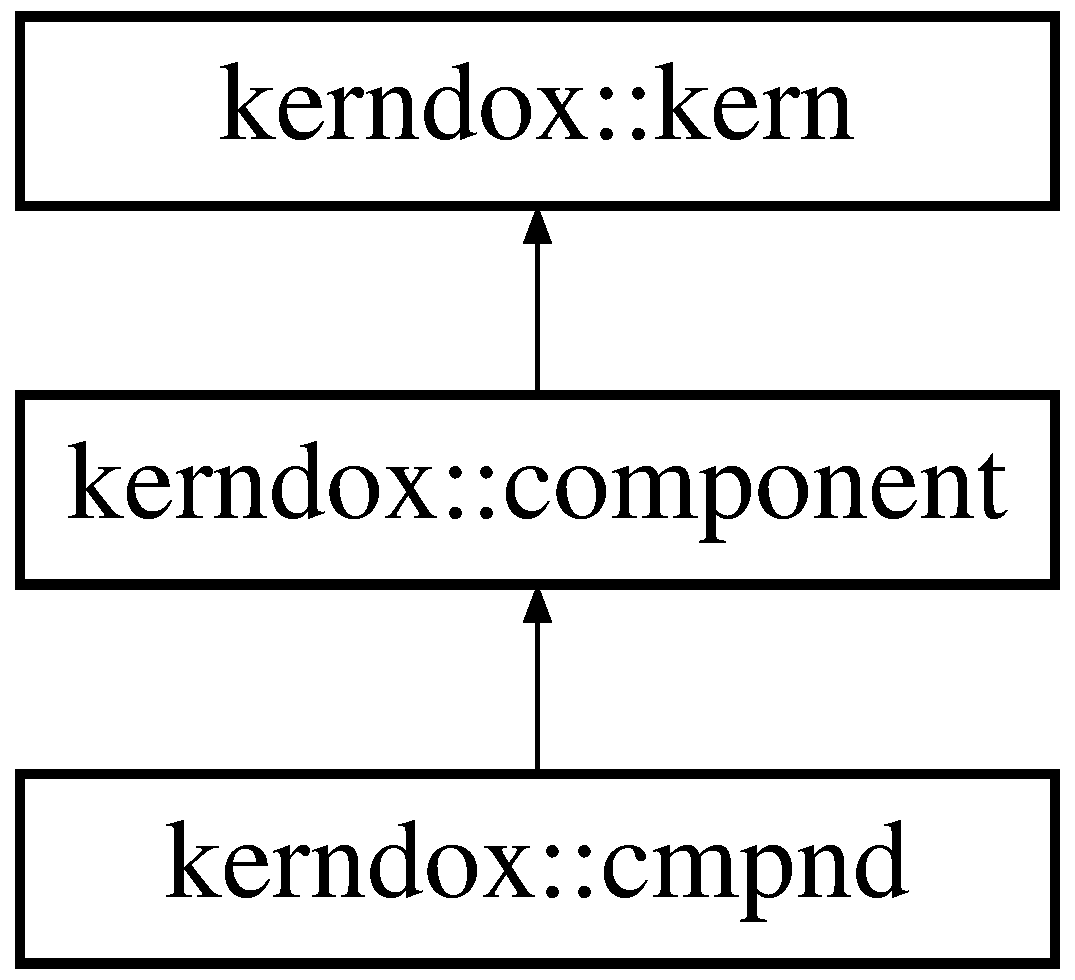
\includegraphics[height=3cm]{classkerndox_1_1cmpnd}
\end{center}
\end{figure}
\subsection*{Public Member Functions}
\begin{CompactItemize}
\item 
\hypertarget{classkerndox_1_1cmpnd_d5d41d9195f7265a1684d4d1fd56d628}{
def \textbf{\_\-\_\-init\_\-\_\-}}
\label{classkerndox_1_1cmpnd_d5d41d9195f7265a1684d4d1fd56d628}

\item 
\hypertarget{classkerndox_1_1cmpnd_64a64b380f404eb289618bc1d9b4d7bf}{
def \textbf{paramInit}}
\label{classkerndox_1_1cmpnd_64a64b380f404eb289618bc1d9b4d7bf}

\item 
\hypertarget{classkerndox_1_1cmpnd_35e6ac83918427bcaf841711584899c2}{
def \textbf{compute}}
\label{classkerndox_1_1cmpnd_35e6ac83918427bcaf841711584899c2}

\item 
def \hyperlink{classkerndox_1_1cmpnd_7d72493b41b96c0609578f099c645502}{diagCompute}
\item 
def \hyperlink{classkerndox_1_1cmpnd_7d38f78fb440a79986244a97af3ecdef}{diagGradX}
\item 
def \hyperlink{classkerndox_1_1cmpnd_0e17dcc7e3bde7bec100461fcc4a6bb4}{diagGradient}
\item 
def \hyperlink{classkerndox_1_1cmpnd_e7de55282e4d0f93d66642f887da6544}{display}
\item 
def \hyperlink{classkerndox_1_1cmpnd_64fb3d184567fe23f6dd7be1797e8a05}{gradX}
\item 
def \hyperlink{classkerndox_1_1cmpnd_029858b6168a89349a61d417ffe99fbd}{gradient}
\item 
def \hyperlink{classkerndox_1_1cmpnd_cc6c3c268042f3e7f7bf8ec1cccd17cf}{expandParam}
\item 
def \hyperlink{classkerndox_1_1cmpnd_a93cf33b23fb72063f34423a7f738d4e}{extractParam}
\item 
def \hyperlink{classkerndox_1_1cmpnd_15e6fbd563d2d6784c353ed8c9064792}{extractParamNames}
\end{CompactItemize}
\subsection*{Public Attributes}
\begin{CompactItemize}
\item 
\hypertarget{classkerndox_1_1cmpnd_f2b47be8a728ecdc7f72147d386bd38d}{
\textbf{type}}
\label{classkerndox_1_1cmpnd_f2b47be8a728ecdc7f72147d386bd38d}

\item 
\hypertarget{classkerndox_1_1cmpnd_728be225e33829677518a682bc8fbd31}{
\textbf{stationary}}
\label{classkerndox_1_1cmpnd_728be225e33829677518a682bc8fbd31}

\item 
\hypertarget{classkerndox_1_1cmpnd_d4bf8795eac773b70d19b9af0098d11a}{
\textbf{whiteVariance}}
\label{classkerndox_1_1cmpnd_d4bf8795eac773b70d19b9af0098d11a}

\end{CompactItemize}


\subsection{Detailed Description}


\footnotesize\begin{verbatim}The is short for compound kernel and it is developed
by summing several kernels together.\end{verbatim}
\normalsize
 

\subsection{Member Function Documentation}
\hypertarget{classkerndox_1_1cmpnd_7d72493b41b96c0609578f099c645502}{
\index{kerndox::cmpnd@{kerndox::cmpnd}!diagCompute@{diagCompute}}
\index{diagCompute@{diagCompute}!kerndox::cmpnd@{kerndox::cmpnd}}
\subsubsection[{diagCompute}]{\setlength{\rightskip}{0pt plus 5cm}def kerndox::cmpnd::diagCompute ( {\em self}, \/   {\em x})}}
\label{classkerndox_1_1cmpnd_7d72493b41b96c0609578f099c645502}




\footnotesize\begin{verbatim}DIAGCOMPUTE Compute diagonal of CMPND kernel.
FORMAT
DESC computes the diagonal of the kernel matrix for the
compound kernel given a design matrix of inputs.
\param kern : the kernel structure for which the matrix is computed.
\param x : input data matrix in the form of a design matrix.
\return  k : a vector containing the diagonal of the kernel matrix
computed at the given points.
%
SEEALSO : cmpndKernParamInit, kernDiagCompute, create, cmpndKernCompute
%
COPYRIGHT : Neil D. Lawrence, 2004, 2005, 2006, 2009

\end{verbatim}
\normalsize
 

Reimplemented from \hyperlink{classkerndox_1_1kern}{kerndox::kern}.\hypertarget{classkerndox_1_1cmpnd_0e17dcc7e3bde7bec100461fcc4a6bb4}{
\index{kerndox::cmpnd@{kerndox::cmpnd}!diagGradient@{diagGradient}}
\index{diagGradient@{diagGradient}!kerndox::cmpnd@{kerndox::cmpnd}}
\subsubsection[{diagGradient}]{\setlength{\rightskip}{0pt plus 5cm}def kerndox::cmpnd::diagGradient ( {\em self}, \/   {\em x}, \/   {\em covDiag})}}
\label{classkerndox_1_1cmpnd_0e17dcc7e3bde7bec100461fcc4a6bb4}




\footnotesize\begin{verbatim}DIAGGRADIENT Compute the gradient of the CMPND kernel's diagonal wrt parameters.
FORMAT
DESC computes the gradient of functions of the diagonal of the
compound kernel matrix with respect to the parameters of the kernel. The
parameters' gradients are returned in the order given by the
cmpndKernExtractParam command.
\param kern : the kernel structure for which the gradients are
computed.
\param x : the input data for which the gradient is being computed.
\param factors : partial derivatives of the function of interest with
respect to the diagonal elements of the kernel.
\return  g : gradients of the relevant function with respect to each
of the parameters. Ordering should match the ordering given in
cmpndKernExtractParam.
%
SEEALSO : cmpndKernParamInit, kernDiagGradient, cmpndKernExtractParam, cmpndKernGradient
%
COPYRIGHT : Neil D. Lawrence, 2004, 2005, 2006, 2009

\end{verbatim}
\normalsize
 

Reimplemented from \hyperlink{classkerndox_1_1kern}{kerndox::kern}.\hypertarget{classkerndox_1_1cmpnd_7d38f78fb440a79986244a97af3ecdef}{
\index{kerndox::cmpnd@{kerndox::cmpnd}!diagGradX@{diagGradX}}
\index{diagGradX@{diagGradX}!kerndox::cmpnd@{kerndox::cmpnd}}
\subsubsection[{diagGradX}]{\setlength{\rightskip}{0pt plus 5cm}def kerndox::cmpnd::diagGradX ( {\em self}, \/   {\em X})}}
\label{classkerndox_1_1cmpnd_7d38f78fb440a79986244a97af3ecdef}




\footnotesize\begin{verbatim}DIAGGRADX Gradient of CMPND kernel's diagonal with respect to X.
FORMAT
DESC computes the gradient of the diagonal of the compound kernel matrix with
respect to the elements of the design matrix given in X.
\param kern : the kernel structure for which gradients are being computed.
\param X : the input data in the form of a design matrix.
\return  gX : the gradients of the diagonal with respect to each element
of X. The returned matrix has the same dimensions as X.
%
SEEALSO : cmpndKernParamInit, kernDiagGradX, cmpndkernGradX
%
COPYRIGHT : Neil D. Lawrence, 2004, 2005, 2006, 2009

\end{verbatim}
\normalsize
 

Reimplemented from \hyperlink{classkerndox_1_1kern}{kerndox::kern}.\hypertarget{classkerndox_1_1cmpnd_e7de55282e4d0f93d66642f887da6544}{
\index{kerndox::cmpnd@{kerndox::cmpnd}!display@{display}}
\index{display@{display}!kerndox::cmpnd@{kerndox::cmpnd}}
\subsubsection[{display}]{\setlength{\rightskip}{0pt plus 5cm}def kerndox::cmpnd::display ( {\em self}, \/   {\em numSpaces} = {\tt 0})}}
\label{classkerndox_1_1cmpnd_e7de55282e4d0f93d66642f887da6544}




\footnotesize\begin{verbatim}DISPLAY Display parameters of the CMPND kernel.
FORMAT
DESC displays the parameters of the compound
kernel and the kernel type to the console.
\param kern : the kernel to display.
%
FORMAT does the same as above, but indents the display according
to the amount specified.
\param kern : the kernel to display.
\param spacing : how many spaces to indent the display of the kernel by.
%
SEEALSO : cmpndKernParamInit, modelDisplay, kernDisplay
%
COPYRIGHT : Neil D. Lawrence, 2004, 2005, 2006, 2009

\end{verbatim}
\normalsize
 

Reimplemented from \hyperlink{classkerndox_1_1kern}{kerndox::kern}.\hypertarget{classkerndox_1_1cmpnd_cc6c3c268042f3e7f7bf8ec1cccd17cf}{
\index{kerndox::cmpnd@{kerndox::cmpnd}!expandParam@{expandParam}}
\index{expandParam@{expandParam}!kerndox::cmpnd@{kerndox::cmpnd}}
\subsubsection[{expandParam}]{\setlength{\rightskip}{0pt plus 5cm}def kerndox::cmpnd::expandParam ( {\em self}, \/   {\em params})}}
\label{classkerndox_1_1cmpnd_cc6c3c268042f3e7f7bf8ec1cccd17cf}




\footnotesize\begin{verbatim}EXPANDPARAM Create kernel structure from CMPND kernel's parameters.
FORMAT
DESC returns a compound kernel structure filled with the
parameters in the given vector. This is used as a helper function to
enable parameters to be optimised in, for example, the NETLAB
optimisation functions.
\param kern : the kernel structure in which the parameters are to be
placed.
\param param : vector of parameters which are to be placed in the
kernel structure.
\return  kern : kernel structure with the given parameters in the
relevant locations.
%
SEEALSO : cmpndKernParamInit, cmpndKernExtractParam, kernExpandParam
%
COPYRIGHT : Neil D. Lawrence, 2004, 2005, 2006, 2009

\end{verbatim}
\normalsize
 \hypertarget{classkerndox_1_1cmpnd_a93cf33b23fb72063f34423a7f738d4e}{
\index{kerndox::cmpnd@{kerndox::cmpnd}!extractParam@{extractParam}}
\index{extractParam@{extractParam}!kerndox::cmpnd@{kerndox::cmpnd}}
\subsubsection[{extractParam}]{\setlength{\rightskip}{0pt plus 5cm}def kerndox::cmpnd::extractParam ( {\em self})}}
\label{classkerndox_1_1cmpnd_a93cf33b23fb72063f34423a7f738d4e}




\footnotesize\begin{verbatim}EXTRACTPARAM Extract parameters from the CMPND kernel structure.
FORMAT
DESC Extract parameters from the compound kernel matrix into a vector of
parameters for optimisation.
\param kern : the kernel structure containing the parameters to be
extracted.
\return  param : vector of parameters extracted from the
kernel. The vector of 'transforms' is assumed to be empty
here. Any transformations of parameters should be done in
component kernels.
%
SEEALSO cmpndKernParamInit, cmpndKernExpandParam, kernExtractParam, scg, conjgrad
%
COPYRIGHT : Neil D. Lawrence, 2004, 2005, 2006, 2009

\end{verbatim}
\normalsize
 \hypertarget{classkerndox_1_1cmpnd_15e6fbd563d2d6784c353ed8c9064792}{
\index{kerndox::cmpnd@{kerndox::cmpnd}!extractParamNames@{extractParamNames}}
\index{extractParamNames@{extractParamNames}!kerndox::cmpnd@{kerndox::cmpnd}}
\subsubsection[{extractParamNames}]{\setlength{\rightskip}{0pt plus 5cm}def kerndox::cmpnd::extractParamNames ( {\em self})}}
\label{classkerndox_1_1cmpnd_15e6fbd563d2d6784c353ed8c9064792}




\footnotesize\begin{verbatim}EXTRACTPARAMNAMES Extract parameter names from the CMPND kernel structure.
FORMAT
DESC Extract parameters from the compound kernel matrix into a vector of
parameters for optimisation.
\param kern : the kernel structure containing the parameters to be
extracted.
\return  names : a list of parameter names.
%
SEEALSO cmpndKernParamInit, cmpndKernExpandParam, kernExtractParam, scg, conjgrad
%
COPYRIGHT : Neil D. Lawrence, 2004, 2005, 2006, 2009

\end{verbatim}
\normalsize
 \hypertarget{classkerndox_1_1cmpnd_029858b6168a89349a61d417ffe99fbd}{
\index{kerndox::cmpnd@{kerndox::cmpnd}!gradient@{gradient}}
\index{gradient@{gradient}!kerndox::cmpnd@{kerndox::cmpnd}}
\subsubsection[{gradient}]{\setlength{\rightskip}{0pt plus 5cm}def kerndox::cmpnd::gradient ( {\em self}, \/   {\em X}, \/   {\em X2} = {\tt None}, \/   {\em covGrad} = {\tt None})}}
\label{classkerndox_1_1cmpnd_029858b6168a89349a61d417ffe99fbd}




\footnotesize\begin{verbatim}GRADIENT Gradient of CMPND kernel's parameters.
FORMAT
DESC computes the gradient of functions with respect to the
compound
kernel's parameters. As well as the kernel structure and the
input positions, the user provides a matrix PARTIAL which gives
the partial derivatives of the function with respect to the
relevant elements of the kernel matrix. 
\param kern : the kernel structure for which the gradients are being
computed.
\param x : the input locations for which the gradients are being
computed. 
\param partial : matrix of partial derivatives of the function of
interest with respect to the kernel matrix. The argument takes
the form of a square matrix of dimension  numData, where numData is
the number of rows in X.
\return  g : gradients of the function of interest with respect to
the kernel parameters. The ordering of the vector should match
that provided by the function kernExtractParam.
%
FORMAT
DESC computes the derivatives as above, but input locations are
now provided in two matrices associated with rows and columns of
the kernel matrix. 
\param kern : the kernel structure for which the gradients are being
computed.
\param x1 : the input locations associated with the rows of the
kernel matrix.
\param x2 : the input locations associated with the columns of the
kernel matrix.
\param partial : matrix of partial derivatives of the function of
interest with respect to the kernel matrix. The matrix should
have the same number of rows as X1 and the same number of columns
as X2 has rows.
\return  g : gradients of the function of interest with respect to
the kernel parameters.
%
SEEALSO cmpndKernParamInit, kernGradient, cmpndKernDiagGradient, kernGradX
%
COPYRIGHT : Neil D. Lawrence, 2004, 2005, 2006, 2009

\end{verbatim}
\normalsize
 

Reimplemented from \hyperlink{classkerndox_1_1kern}{kerndox::kern}.\hypertarget{classkerndox_1_1cmpnd_64fb3d184567fe23f6dd7be1797e8a05}{
\index{kerndox::cmpnd@{kerndox::cmpnd}!gradX@{gradX}}
\index{gradX@{gradX}!kerndox::cmpnd@{kerndox::cmpnd}}
\subsubsection[{gradX}]{\setlength{\rightskip}{0pt plus 5cm}def kerndox::cmpnd::gradX ( {\em self}, \/   {\em X}, \/   {\em X2})}}
\label{classkerndox_1_1cmpnd_64fb3d184567fe23f6dd7be1797e8a05}




\footnotesize\begin{verbatim}GRADX Gradient of CMPND kernel with respect to a point x.
FORMAT
DESC computes the gradient of the compound
kernel with respect to the input positions. 
\param kern : kernel structure for which gradients are being
computed.
\param x : locations against which gradients are being computed.
\return  g : the returned gradients. The gradients are returned in
a matrix which is numData x numInputs x numData. Where numData is
the number of data points and numInputs is the number of input
dimensions in X.
%
FORMAT
DESC computes the gradident of the compound
kernel with respect to the input positions where both the row
positions and column positions are provided separately.
\param kern : kernel structure for which gradients are being
computed.
\param x1 : row locations against which gradients are being computed.
\param x2 : column locations against which gradients are being computed.
\return  g : the returned gradients. The gradients are returned in
a matrix which is numData2 x numInputs x numData1. Where numData1 is
the number of data points in X1, numData2 is the number of data
points in X2 and numInputs is the number of input
dimensions in X.
%
SEEALSO cmpndKernParamInit, kernGradX, cmpndKernDiagGradX
%
COPYRIGHT : Neil D. Lawrence, 2004, 2005, 2006, 2009

\end{verbatim}
\normalsize
 

Reimplemented from \hyperlink{classkerndox_1_1kern}{kerndox::kern}.

The documentation for this class was generated from the following file:\begin{CompactItemize}
\item 
kerndox.py\end{CompactItemize}

\hypertarget{classkern_1_1cmpnd}{
\section{kern::cmpnd Class Reference}
\label{classkern_1_1cmpnd}\index{kern::cmpnd@{kern::cmpnd}}
}
Inheritance diagram for kern::cmpnd::\begin{figure}[H]
\begin{center}
\leavevmode
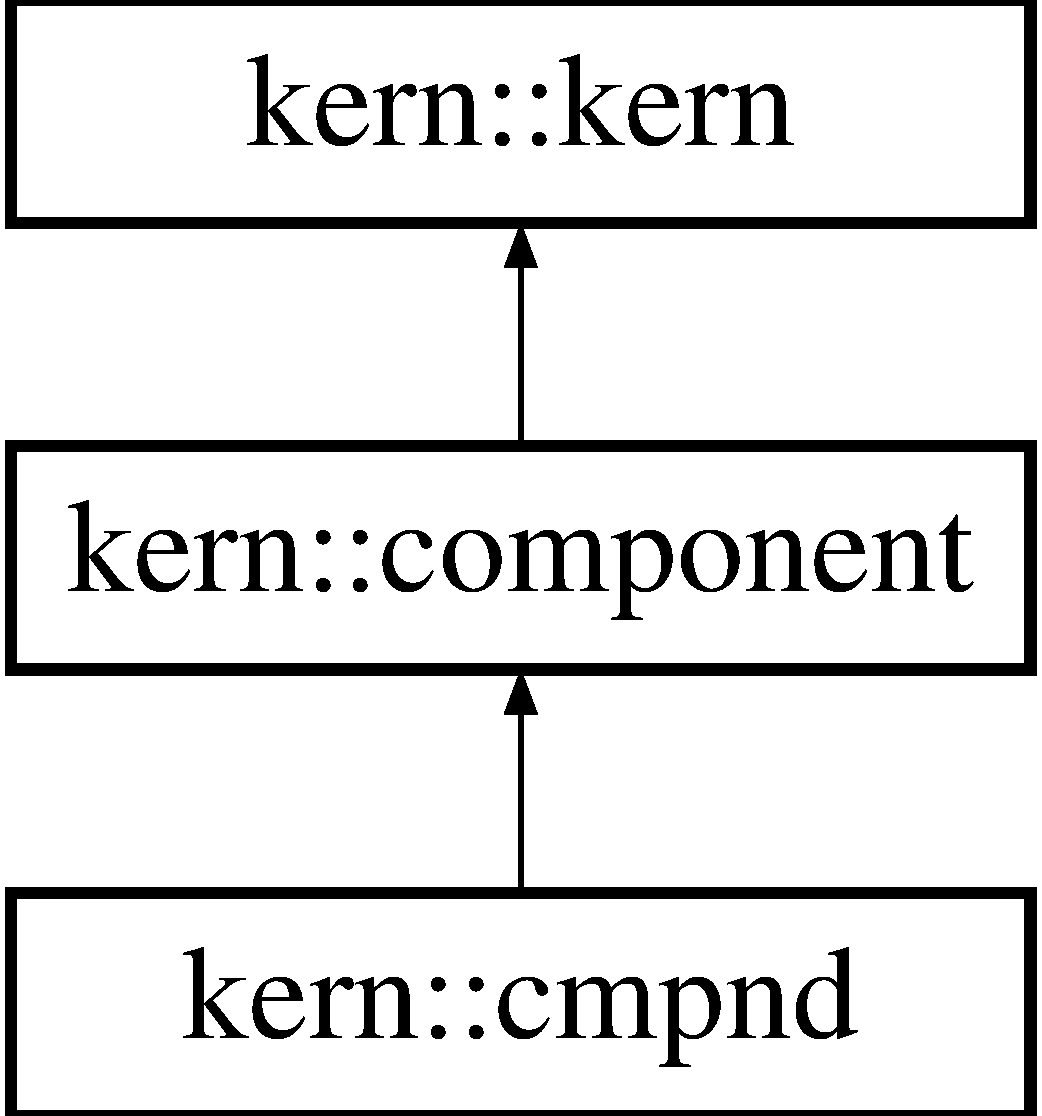
\includegraphics[height=3cm]{classkern_1_1cmpnd}
\end{center}
\end{figure}
\subsection*{Public Member Functions}
\begin{CompactItemize}
\item 
\hypertarget{classkern_1_1cmpnd_ae3454cc98bd9dee5aca8e026aeb3f39}{
def \textbf{\_\-\_\-init\_\-\_\-}}
\label{classkern_1_1cmpnd_ae3454cc98bd9dee5aca8e026aeb3f39}

\item 
\hypertarget{classkern_1_1cmpnd_75661bd9826c15420989baef60f37983}{
def \textbf{paramInit}}
\label{classkern_1_1cmpnd_75661bd9826c15420989baef60f37983}

\item 
\hypertarget{classkern_1_1cmpnd_2cd292ccfbaee98ed2988bb88673f235}{
def \textbf{compute}}
\label{classkern_1_1cmpnd_2cd292ccfbaee98ed2988bb88673f235}

\item 
def \hyperlink{classkern_1_1cmpnd_5852fb0a16565b8a888c5b32399a0abd}{diagCompute}
\item 
def \hyperlink{classkern_1_1cmpnd_fa9a662412350b04289be9554bfd2b6e}{diagGradX}
\item 
def \hyperlink{classkern_1_1cmpnd_9ae8217ccbe28caeaa509ee33123c67a}{diagGradient}
\item 
def \hyperlink{classkern_1_1cmpnd_5f0881b786c5ffcf0262732c8f119d1a}{display}
\item 
def \hyperlink{classkern_1_1cmpnd_ae07d88bf593fd048c2a0464bfd923b8}{gradX}
\item 
def \hyperlink{classkern_1_1cmpnd_bae88f1fa7e84fa6d7651313460d35fc}{gradient}
\item 
def \hyperlink{classkern_1_1cmpnd_4fa764e9b24f54a8eb3ee05f07983452}{expandParam}
\item 
def \hyperlink{classkern_1_1cmpnd_318f984498fc390d902dd5bc2358cf66}{extractParam}
\item 
def \hyperlink{classkern_1_1cmpnd_265822a277cefcadc62b50c5a4f2cc1a}{extractParamNames}
\end{CompactItemize}
\subsection*{Public Attributes}
\begin{CompactItemize}
\item 
\hypertarget{classkern_1_1cmpnd_c9b5eb3435c417c472cadb0644eb3fbc}{
\textbf{type}}
\label{classkern_1_1cmpnd_c9b5eb3435c417c472cadb0644eb3fbc}

\item 
\hypertarget{classkern_1_1cmpnd_18f301cebf729f9c905ba52e0ab1c3f1}{
\textbf{stationary}}
\label{classkern_1_1cmpnd_18f301cebf729f9c905ba52e0ab1c3f1}

\item 
\hypertarget{classkern_1_1cmpnd_c470399a334eada7a278bc914e39ddd3}{
\textbf{whiteVariance}}
\label{classkern_1_1cmpnd_c470399a334eada7a278bc914e39ddd3}

\end{CompactItemize}


\subsection{Detailed Description}


\footnotesize\begin{verbatim}The is short for compound kernel and it is developed
by summing several kernels together.\end{verbatim}
\normalsize
 

\subsection{Member Function Documentation}
\hypertarget{classkern_1_1cmpnd_5852fb0a16565b8a888c5b32399a0abd}{
\index{kern::cmpnd@{kern::cmpnd}!diagCompute@{diagCompute}}
\index{diagCompute@{diagCompute}!kern::cmpnd@{kern::cmpnd}}
\subsubsection[{diagCompute}]{\setlength{\rightskip}{0pt plus 5cm}def kern::cmpnd::diagCompute ( {\em self}, \/   {\em x})}}
\label{classkern_1_1cmpnd_5852fb0a16565b8a888c5b32399a0abd}




\footnotesize\begin{verbatim}% DIAGCOMPUTE Compute diagonal of CMPND kernel.
% FORMAT
% DESC computes the diagonal of the kernel matrix for the
% compound kernel given a design matrix of inputs.
% ARG kern : the kernel structure for which the matrix is computed.
% ARG x : input data matrix in the form of a design matrix.
% RETURN k : a vector containing the diagonal of the kernel matrix
% computed at the given points.
%
% SEEALSO : cmpndKernParamInit, kernDiagCompute, create, cmpndKernCompute
%
% COPYRIGHT : Neil D. Lawrence, 2004, 2005, 2006, 2009

\end{verbatim}
\normalsize
 

Reimplemented from \hyperlink{classkern_1_1kern}{kern::kern}.\hypertarget{classkern_1_1cmpnd_9ae8217ccbe28caeaa509ee33123c67a}{
\index{kern::cmpnd@{kern::cmpnd}!diagGradient@{diagGradient}}
\index{diagGradient@{diagGradient}!kern::cmpnd@{kern::cmpnd}}
\subsubsection[{diagGradient}]{\setlength{\rightskip}{0pt plus 5cm}def kern::cmpnd::diagGradient ( {\em self}, \/   {\em x}, \/   {\em covDiag})}}
\label{classkern_1_1cmpnd_9ae8217ccbe28caeaa509ee33123c67a}




\footnotesize\begin{verbatim}% DIAGGRADIENT Compute the gradient of the CMPND kernel's diagonal wrt parameters.
% FORMAT
% DESC computes the gradient of functions of the diagonal of the
% compound kernel matrix with respect to the parameters of the kernel. The
% parameters' gradients are returned in the order given by the
% cmpndKernExtractParam command.
% ARG kern : the kernel structure for which the gradients are
% computed.
% ARG x : the input data for which the gradient is being computed.
% ARG factors : partial derivatives of the function of interest with
% respect to the diagonal elements of the kernel.
% RETURN g : gradients of the relevant function with respect to each
% of the parameters. Ordering should match the ordering given in
% cmpndKernExtractParam.
%
% SEEALSO : cmpndKernParamInit, kernDiagGradient, cmpndKernExtractParam, cmpndKernGradient
%
% COPYRIGHT : Neil D. Lawrence, 2004, 2005, 2006, 2009

\end{verbatim}
\normalsize
 

Reimplemented from \hyperlink{classkern_1_1kern}{kern::kern}.\hypertarget{classkern_1_1cmpnd_fa9a662412350b04289be9554bfd2b6e}{
\index{kern::cmpnd@{kern::cmpnd}!diagGradX@{diagGradX}}
\index{diagGradX@{diagGradX}!kern::cmpnd@{kern::cmpnd}}
\subsubsection[{diagGradX}]{\setlength{\rightskip}{0pt plus 5cm}def kern::cmpnd::diagGradX ( {\em self}, \/   {\em X})}}
\label{classkern_1_1cmpnd_fa9a662412350b04289be9554bfd2b6e}




\footnotesize\begin{verbatim}% DIAGGRADX Gradient of CMPND kernel's diagonal with respect to X.
% FORMAT
% DESC computes the gradient of the diagonal of the compound kernel matrix with
% respect to the elements of the design matrix given in X.
% ARG kern : the kernel structure for which gradients are being computed.
% ARG X : the input data in the form of a design matrix.
% RETURN gX : the gradients of the diagonal with respect to each element
% of X. The returned matrix has the same dimensions as X.
%
% SEEALSO : cmpndKernParamInit, kernDiagGradX, cmpndkernGradX
%
% COPYRIGHT : Neil D. Lawrence, 2004, 2005, 2006, 2009

\end{verbatim}
\normalsize
 

Reimplemented from \hyperlink{classkern_1_1kern}{kern::kern}.\hypertarget{classkern_1_1cmpnd_5f0881b786c5ffcf0262732c8f119d1a}{
\index{kern::cmpnd@{kern::cmpnd}!display@{display}}
\index{display@{display}!kern::cmpnd@{kern::cmpnd}}
\subsubsection[{display}]{\setlength{\rightskip}{0pt plus 5cm}def kern::cmpnd::display ( {\em self}, \/   {\em numSpaces} = {\tt 0})}}
\label{classkern_1_1cmpnd_5f0881b786c5ffcf0262732c8f119d1a}




\footnotesize\begin{verbatim}% DISPLAY Display parameters of the CMPND kernel.
% FORMAT
% DESC displays the parameters of the compound
% kernel and the kernel type to the console.
% ARG kern : the kernel to display.
%
% FORMAT does the same as above, but indents the display according
% to the amount specified.
% ARG kern : the kernel to display.
% ARG spacing : how many spaces to indent the display of the kernel by.
%
% SEEALSO : cmpndKernParamInit, modelDisplay, kernDisplay
%
% COPYRIGHT : Neil D. Lawrence, 2004, 2005, 2006, 2009

\end{verbatim}
\normalsize
 

Reimplemented from \hyperlink{classkern_1_1kern}{kern::kern}.\hypertarget{classkern_1_1cmpnd_4fa764e9b24f54a8eb3ee05f07983452}{
\index{kern::cmpnd@{kern::cmpnd}!expandParam@{expandParam}}
\index{expandParam@{expandParam}!kern::cmpnd@{kern::cmpnd}}
\subsubsection[{expandParam}]{\setlength{\rightskip}{0pt plus 5cm}def kern::cmpnd::expandParam ( {\em self}, \/   {\em params})}}
\label{classkern_1_1cmpnd_4fa764e9b24f54a8eb3ee05f07983452}




\footnotesize\begin{verbatim}% EXPANDPARAM Create kernel structure from CMPND kernel's parameters.
% FORMAT
% DESC returns a compound kernel structure filled with the
% parameters in the given vector. This is used as a helper function to
% enable parameters to be optimised in, for example, the NETLAB
% optimisation functions.
% ARG kern : the kernel structure in which the parameters are to be
% placed.
% ARG param : vector of parameters which are to be placed in the
% kernel structure.
% RETURN kern : kernel structure with the given parameters in the
% relevant locations.
%
% SEEALSO : cmpndKernParamInit, cmpndKernExtractParam, kernExpandParam
%
% COPYRIGHT : Neil D. Lawrence, 2004, 2005, 2006, 2009

\end{verbatim}
\normalsize
 \hypertarget{classkern_1_1cmpnd_318f984498fc390d902dd5bc2358cf66}{
\index{kern::cmpnd@{kern::cmpnd}!extractParam@{extractParam}}
\index{extractParam@{extractParam}!kern::cmpnd@{kern::cmpnd}}
\subsubsection[{extractParam}]{\setlength{\rightskip}{0pt plus 5cm}def kern::cmpnd::extractParam ( {\em self})}}
\label{classkern_1_1cmpnd_318f984498fc390d902dd5bc2358cf66}




\footnotesize\begin{verbatim}% EXTRACTPARAM Extract parameters from the CMPND kernel structure.
% FORMAT
% DESC Extract parameters from the compound kernel matrix into a vector of
% parameters for optimisation.
% ARG kern : the kernel structure containing the parameters to be
% extracted.
% RETURN param : vector of parameters extracted from the
% kernel. The vector of 'transforms' is assumed to be empty
% here. Any transformations of parameters should be done in
% component kernels.
%
% SEEALSO cmpndKernParamInit, cmpndKernExpandParam, kernExtractParam, scg, conjgrad
%
% COPYRIGHT : Neil D. Lawrence, 2004, 2005, 2006, 2009

\end{verbatim}
\normalsize
 \hypertarget{classkern_1_1cmpnd_265822a277cefcadc62b50c5a4f2cc1a}{
\index{kern::cmpnd@{kern::cmpnd}!extractParamNames@{extractParamNames}}
\index{extractParamNames@{extractParamNames}!kern::cmpnd@{kern::cmpnd}}
\subsubsection[{extractParamNames}]{\setlength{\rightskip}{0pt plus 5cm}def kern::cmpnd::extractParamNames ( {\em self})}}
\label{classkern_1_1cmpnd_265822a277cefcadc62b50c5a4f2cc1a}




\footnotesize\begin{verbatim}% EXTRACTPARAMNAMES Extract parameter names from the CMPND kernel structure.
% FORMAT
% DESC Extract parameters from the compound kernel matrix into a vector of
% parameters for optimisation.
% ARG kern : the kernel structure containing the parameters to be
% extracted.
% RETURN names : a list of parameter names.
%
% SEEALSO cmpndKernParamInit, cmpndKernExpandParam, kernExtractParam, scg, conjgrad
%
% COPYRIGHT : Neil D. Lawrence, 2004, 2005, 2006, 2009

\end{verbatim}
\normalsize
 \hypertarget{classkern_1_1cmpnd_bae88f1fa7e84fa6d7651313460d35fc}{
\index{kern::cmpnd@{kern::cmpnd}!gradient@{gradient}}
\index{gradient@{gradient}!kern::cmpnd@{kern::cmpnd}}
\subsubsection[{gradient}]{\setlength{\rightskip}{0pt plus 5cm}def kern::cmpnd::gradient ( {\em self}, \/   {\em X}, \/   {\em X2} = {\tt None}, \/   {\em covGrad} = {\tt None})}}
\label{classkern_1_1cmpnd_bae88f1fa7e84fa6d7651313460d35fc}




\footnotesize\begin{verbatim}% GRADIENT Gradient of CMPND kernel's parameters.
% FORMAT
% DESC computes the gradient of functions with respect to the
% compound
% kernel's parameters. As well as the kernel structure and the
% input positions, the user provides a matrix PARTIAL which gives
% the partial derivatives of the function with respect to the
% relevant elements of the kernel matrix. 
% ARG kern : the kernel structure for which the gradients are being
% computed.
% ARG x : the input locations for which the gradients are being
% computed. 
% ARG partial : matrix of partial derivatives of the function of
% interest with respect to the kernel matrix. The argument takes
% the form of a square matrix of dimension  numData, where numData is
% the number of rows in X.
% RETURN g : gradients of the function of interest with respect to
% the kernel parameters. The ordering of the vector should match
% that provided by the function kernExtractParam.
%
% FORMAT
% DESC computes the derivatives as above, but input locations are
% now provided in two matrices associated with rows and columns of
% the kernel matrix. 
% ARG kern : the kernel structure for which the gradients are being
% computed.
% ARG x1 : the input locations associated with the rows of the
% kernel matrix.
% ARG x2 : the input locations associated with the columns of the
% kernel matrix.
% ARG partial : matrix of partial derivatives of the function of
% interest with respect to the kernel matrix. The matrix should
% have the same number of rows as X1 and the same number of columns
% as X2 has rows.
% RETURN g : gradients of the function of interest with respect to
% the kernel parameters.
%
% SEEALSO cmpndKernParamInit, kernGradient, cmpndKernDiagGradient, kernGradX
%
% COPYRIGHT : Neil D. Lawrence, 2004, 2005, 2006, 2009

\end{verbatim}
\normalsize
 

Reimplemented from \hyperlink{classkern_1_1kern}{kern::kern}.\hypertarget{classkern_1_1cmpnd_ae07d88bf593fd048c2a0464bfd923b8}{
\index{kern::cmpnd@{kern::cmpnd}!gradX@{gradX}}
\index{gradX@{gradX}!kern::cmpnd@{kern::cmpnd}}
\subsubsection[{gradX}]{\setlength{\rightskip}{0pt plus 5cm}def kern::cmpnd::gradX ( {\em self}, \/   {\em X}, \/   {\em X2})}}
\label{classkern_1_1cmpnd_ae07d88bf593fd048c2a0464bfd923b8}




\footnotesize\begin{verbatim}% GRADX Gradient of CMPND kernel with respect to a point x.
% FORMAT
% DESC computes the gradient of the compound
% kernel with respect to the input positions. 
% ARG kern : kernel structure for which gradients are being
% computed.
% ARG x : locations against which gradients are being computed.
% RETURN g : the returned gradients. The gradients are returned in
% a matrix which is numData x numInputs x numData. Where numData is
% the number of data points and numInputs is the number of input
% dimensions in X.
%
% FORMAT
% DESC computes the gradident of the compound
% kernel with respect to the input positions where both the row
% positions and column positions are provided separately.
% ARG kern : kernel structure for which gradients are being
% computed.
% ARG x1 : row locations against which gradients are being computed.
% ARG x2 : column locations against which gradients are being computed.
% RETURN g : the returned gradients. The gradients are returned in
% a matrix which is numData2 x numInputs x numData1. Where numData1 is
% the number of data points in X1, numData2 is the number of data
% points in X2 and numInputs is the number of input
% dimensions in X.
%
% SEEALSO cmpndKernParamInit, kernGradX, cmpndKernDiagGradX
%
% COPYRIGHT : Neil D. Lawrence, 2004, 2005, 2006, 2009

\end{verbatim}
\normalsize
 

Reimplemented from \hyperlink{classkern_1_1kern}{kern::kern}.

The documentation for this class was generated from the following file:\begin{CompactItemize}
\item 
kern.py\end{CompactItemize}

\hypertarget{classkerndox_1_1component}{
\section{kerndox::component Class Reference}
\label{classkerndox_1_1component}\index{kerndox::component@{kerndox::component}}
}
Inheritance diagram for kerndox::component::\begin{figure}[H]
\begin{center}
\leavevmode
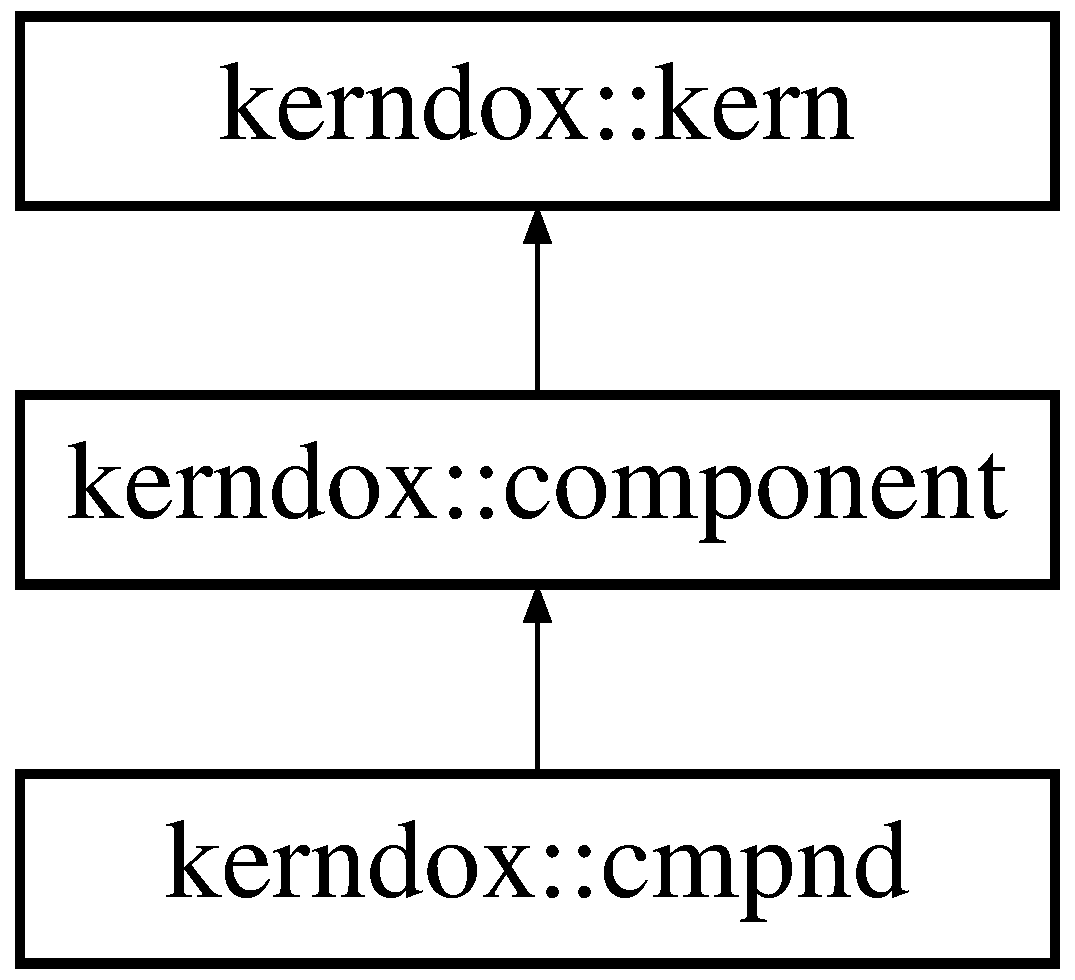
\includegraphics[height=3cm]{classkerndox_1_1component}
\end{center}
\end{figure}
\subsection*{Public Member Functions}
\begin{CompactItemize}
\item 
\hypertarget{classkerndox_1_1component_ed769a067da36c55d8320c84e17b05aa}{
def \textbf{\_\-\_\-init\_\-\_\-}}
\label{classkerndox_1_1component_ed769a067da36c55d8320c84e17b05aa}

\item 
\hypertarget{classkerndox_1_1component_efee2639f6de0fe2abbc3cabb1128ee5}{
def \textbf{addKern}}
\label{classkerndox_1_1component_efee2639f6de0fe2abbc3cabb1128ee5}

\item 
def \hyperlink{classkerndox_1_1component_9ccd80184cbfcf0d09da6f30a3f807ea}{setIndex}
\end{CompactItemize}
\subsection*{Public Attributes}
\begin{CompactItemize}
\item 
\hypertarget{classkerndox_1_1component_196cedc7ce3fd9f482257fff9f59b804}{
\textbf{paramGroups}}
\label{classkerndox_1_1component_196cedc7ce3fd9f482257fff9f59b804}

\item 
\hypertarget{classkerndox_1_1component_4d80eb59597aabe350fa28b5397d6593}{
\textbf{comp}}
\label{classkerndox_1_1component_4d80eb59597aabe350fa28b5397d6593}

\item 
\hypertarget{classkerndox_1_1component_cdfd1f2425d9eb288ce146e9aba8b8bc}{
\textbf{index}}
\label{classkerndox_1_1component_cdfd1f2425d9eb288ce146e9aba8b8bc}

\item 
\hypertarget{classkerndox_1_1component_dc0c595f558a6eb7e0f45bcaf067db2e}{
\textbf{nParams}}
\label{classkerndox_1_1component_dc0c595f558a6eb7e0f45bcaf067db2e}

\item 
\hypertarget{classkerndox_1_1component_64b94412916357ce307f23dbb937bac6}{
\textbf{stationary}}
\label{classkerndox_1_1component_64b94412916357ce307f23dbb937bac6}

\end{CompactItemize}


\subsection{Detailed Description}


\footnotesize\begin{verbatim}The base class for kernels which have several components to
them (such as compound or tensor kernels).

\end{verbatim}
\normalsize
 

\subsection{Member Function Documentation}
\hypertarget{classkerndox_1_1component_9ccd80184cbfcf0d09da6f30a3f807ea}{
\index{kerndox::component@{kerndox::component}!setIndex@{setIndex}}
\index{setIndex@{setIndex}!kerndox::component@{kerndox::component}}
\subsubsection[{setIndex}]{\setlength{\rightskip}{0pt plus 5cm}def kerndox::component::setIndex ( {\em self}, \/   {\em component}, \/   {\em indices})}}
\label{classkerndox_1_1component_9ccd80184cbfcf0d09da6f30a3f807ea}




\footnotesize\begin{verbatim}SETINDEX Set the indices in the compound kernel.

\end{verbatim}
\normalsize
 

The documentation for this class was generated from the following file:\begin{CompactItemize}
\item 
kerndox.py\end{CompactItemize}

\hypertarget{classkern_1_1component}{
\section{kern::component Class Reference}
\label{classkern_1_1component}\index{kern::component@{kern::component}}
}
Inheritance diagram for kern::component::\begin{figure}[H]
\begin{center}
\leavevmode
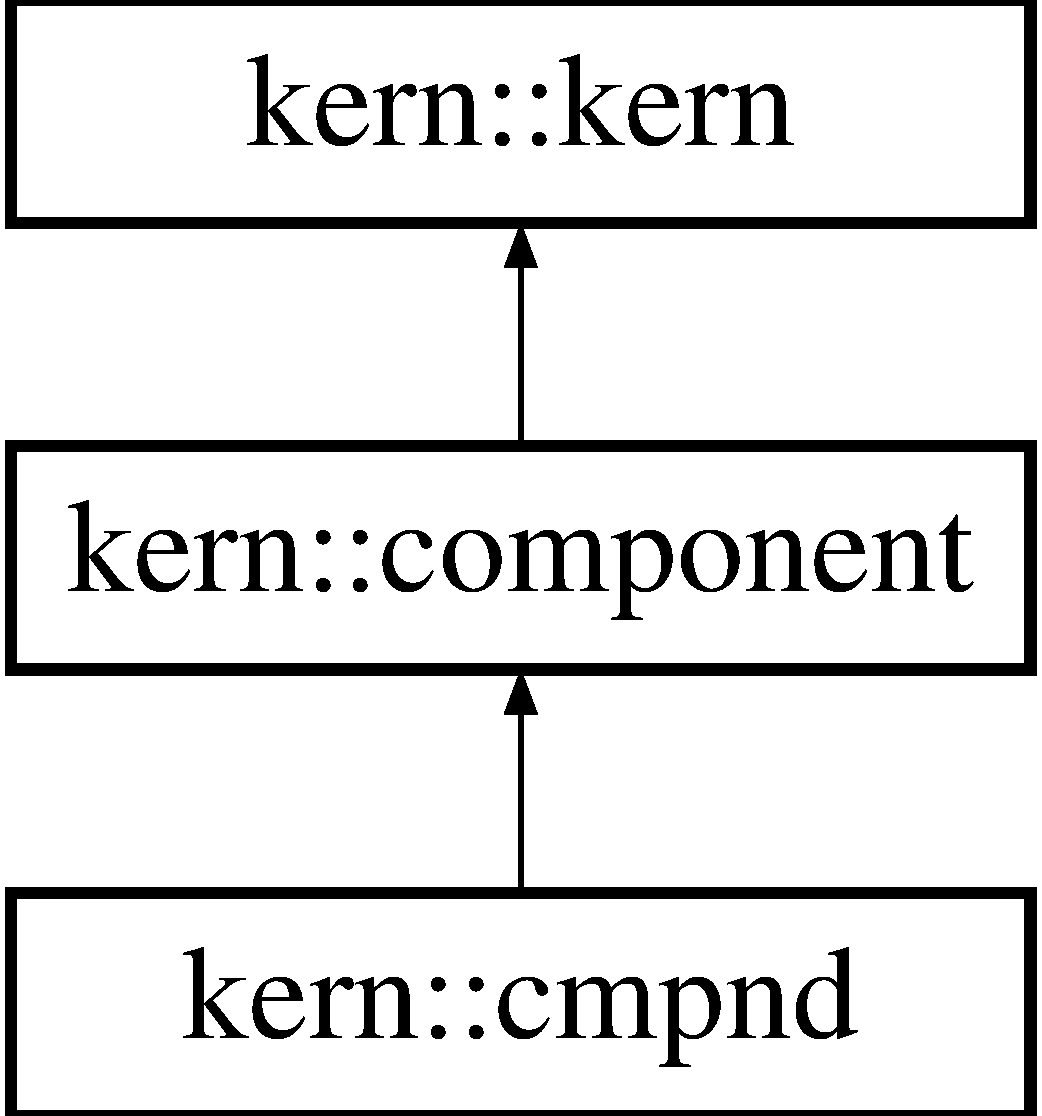
\includegraphics[height=3cm]{classkern_1_1component}
\end{center}
\end{figure}
\subsection*{Public Member Functions}
\begin{CompactItemize}
\item 
\hypertarget{classkern_1_1component_747cbef8e2ac580ae8f43c07889dc382}{
def \textbf{\_\-\_\-init\_\-\_\-}}
\label{classkern_1_1component_747cbef8e2ac580ae8f43c07889dc382}

\item 
\hypertarget{classkern_1_1component_0501a814946c2f941746a2341517bff6}{
def \textbf{addKern}}
\label{classkern_1_1component_0501a814946c2f941746a2341517bff6}

\item 
def \hyperlink{classkern_1_1component_120031427476d451ac010d51833f37e3}{setIndex}
\end{CompactItemize}
\subsection*{Public Attributes}
\begin{CompactItemize}
\item 
\hypertarget{classkern_1_1component_b87e270b4f3b1b3ce51c039557bca0e4}{
\textbf{paramGroups}}
\label{classkern_1_1component_b87e270b4f3b1b3ce51c039557bca0e4}

\item 
\hypertarget{classkern_1_1component_cd02959e911a6abbc0a3d418683062c5}{
\textbf{comp}}
\label{classkern_1_1component_cd02959e911a6abbc0a3d418683062c5}

\item 
\hypertarget{classkern_1_1component_7538e7bd78d86d0cbde04e49fcf22f58}{
\textbf{index}}
\label{classkern_1_1component_7538e7bd78d86d0cbde04e49fcf22f58}

\item 
\hypertarget{classkern_1_1component_97b7665b53ba0cd1ac8123f0287d7d26}{
\textbf{nParams}}
\label{classkern_1_1component_97b7665b53ba0cd1ac8123f0287d7d26}

\item 
\hypertarget{classkern_1_1component_8b2736654a04aebbae1caa61afbfbf3a}{
\textbf{stationary}}
\label{classkern_1_1component_8b2736654a04aebbae1caa61afbfbf3a}

\end{CompactItemize}


\subsection{Detailed Description}


\footnotesize\begin{verbatim}The base class for kernels which have several components to
them (such as compound or tensor kernels).

\end{verbatim}
\normalsize
 

\subsection{Member Function Documentation}
\hypertarget{classkern_1_1component_120031427476d451ac010d51833f37e3}{
\index{kern::component@{kern::component}!setIndex@{setIndex}}
\index{setIndex@{setIndex}!kern::component@{kern::component}}
\subsubsection[{setIndex}]{\setlength{\rightskip}{0pt plus 5cm}def kern::component::setIndex ( {\em self}, \/   {\em component}, \/   {\em indices})}}
\label{classkern_1_1component_120031427476d451ac010d51833f37e3}




\footnotesize\begin{verbatim}SETINDEX Set the indices in the compound kernel.

\end{verbatim}
\normalsize
 

The documentation for this class was generated from the following file:\begin{CompactItemize}
\item 
kern.py\end{CompactItemize}

\hypertarget{classkern_1_1kern}{
\section{kern::kern Class Reference}
\label{classkern_1_1kern}\index{kern::kern@{kern::kern}}
}
Inheritance diagram for kern::kern::\begin{figure}[H]
\begin{center}
\leavevmode
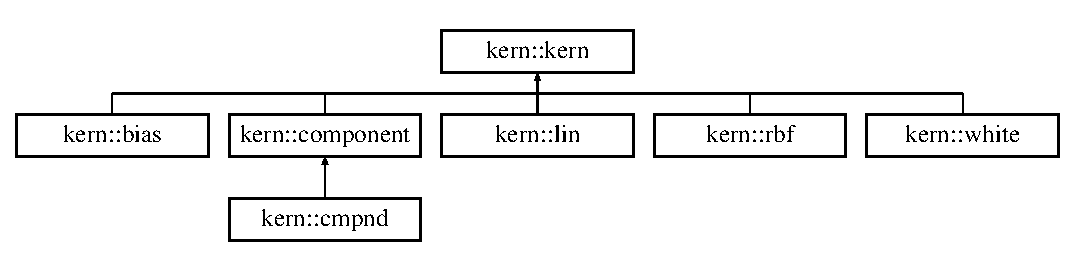
\includegraphics[height=3cm]{classkern_1_1kern}
\end{center}
\end{figure}
\subsection*{Public Member Functions}
\begin{CompactItemize}
\item 
\hypertarget{classkern_1_1kern_55d1483588ace67fd1b3970e1a0ea80b}{
def \textbf{\_\-\_\-init\_\-\_\-}}
\label{classkern_1_1kern_55d1483588ace67fd1b3970e1a0ea80b}

\item 
\hypertarget{classkern_1_1kern_67eee7dd2cf11636e142cece9b82c051}{
def \textbf{paramInit}}
\label{classkern_1_1kern_67eee7dd2cf11636e142cece9b82c051}

\item 
\hypertarget{classkern_1_1kern_6adf6289e897a16d21fa4e3f8dda8a97}{
def \textbf{compute}}
\label{classkern_1_1kern_6adf6289e897a16d21fa4e3f8dda8a97}

\item 
\hypertarget{classkern_1_1kern_5aad6a43fd5c2ed47da04ae0cab41e99}{
def \textbf{diagCompute}}
\label{classkern_1_1kern_5aad6a43fd5c2ed47da04ae0cab41e99}

\item 
\hypertarget{classkern_1_1kern_5a842b523ae8865ce8b1d7e36997343d}{
def \textbf{diagGradX}}
\label{classkern_1_1kern_5a842b523ae8865ce8b1d7e36997343d}

\item 
\hypertarget{classkern_1_1kern_b20b45325bddf066aaf5f1411565f149}{
def \textbf{diagGradient}}
\label{classkern_1_1kern_b20b45325bddf066aaf5f1411565f149}

\item 
\hypertarget{classkern_1_1kern_a0741b54137bf1cbd0aaa85eddcdafcd}{
def \textbf{display}}
\label{classkern_1_1kern_a0741b54137bf1cbd0aaa85eddcdafcd}

\item 
\hypertarget{classkern_1_1kern_c02153c376570b309adceb57110b66c5}{
def \textbf{gradX}}
\label{classkern_1_1kern_c02153c376570b309adceb57110b66c5}

\item 
\hypertarget{classkern_1_1kern_d1a34219fcedf12482207994badde4f5}{
def \textbf{gradient}}
\label{classkern_1_1kern_d1a34219fcedf12482207994badde4f5}

\item 
def \hyperlink{classkern_1_1kern_9cd784d93e47e96eeceda8eecf1be2db}{gradTransParam}
\end{CompactItemize}
\subsection*{Public Attributes}
\begin{CompactItemize}
\item 
\hypertarget{classkern_1_1kern_ca8c12bf8b6d8e82bcdf788a5070ba87}{
\textbf{whiteVariance}}
\label{classkern_1_1kern_ca8c12bf8b6d8e82bcdf788a5070ba87}

\item 
\hypertarget{classkern_1_1kern_40490a9567826e3f96e9f8be3d798ac9}{
\textbf{positiveTime}}
\label{classkern_1_1kern_40490a9567826e3f96e9f8be3d798ac9}

\item 
\hypertarget{classkern_1_1kern_dca0b0f3105db47c0627a0bbc5868001}{
\textbf{inputDimension}}
\label{classkern_1_1kern_dca0b0f3105db47c0627a0bbc5868001}

\end{CompactItemize}


\subsection{Detailed Description}


\footnotesize\begin{verbatim}The base kernel class from which all kernels are derived.\end{verbatim}
\normalsize
 

\subsection{Member Function Documentation}
\hypertarget{classkern_1_1kern_9cd784d93e47e96eeceda8eecf1be2db}{
\index{kern::kern@{kern::kern}!gradTransParam@{gradTransParam}}
\index{gradTransParam@{gradTransParam}!kern::kern@{kern::kern}}
\subsubsection[{gradTransParam}]{\setlength{\rightskip}{0pt plus 5cm}def kern::kern::gradTransParam ( {\em self}, \/   {\em X}, \/   {\em X2} = {\tt None}, \/   {\em covGrad} = {\tt None})}}
\label{classkern_1_1kern_9cd784d93e47e96eeceda8eecf1be2db}




\footnotesize\begin{verbatim}Return the gradient of the transformed parameters.\end{verbatim}
\normalsize
 

The documentation for this class was generated from the following file:\begin{CompactItemize}
\item 
kern.py\end{CompactItemize}

\hypertarget{classkerndox_1_1kern}{
\section{kerndox::kern Class Reference}
\label{classkerndox_1_1kern}\index{kerndox::kern@{kerndox::kern}}
}
Inheritance diagram for kerndox::kern::\begin{figure}[H]
\begin{center}
\leavevmode
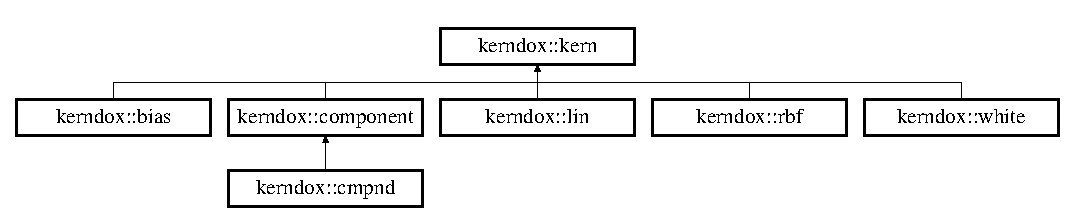
\includegraphics[height=2.54545cm]{classkerndox_1_1kern}
\end{center}
\end{figure}
\subsection*{Public Member Functions}
\begin{CompactItemize}
\item 
\hypertarget{classkerndox_1_1kern_b85f90b813ec151926e34b96680c40b5}{
def \textbf{\_\-\_\-init\_\-\_\-}}
\label{classkerndox_1_1kern_b85f90b813ec151926e34b96680c40b5}

\item 
\hypertarget{classkerndox_1_1kern_b28caeff3b716e12403d699691bb80a3}{
def \textbf{paramInit}}
\label{classkerndox_1_1kern_b28caeff3b716e12403d699691bb80a3}

\item 
\hypertarget{classkerndox_1_1kern_11325240b76ef005012cac80cb7183f8}{
def \textbf{compute}}
\label{classkerndox_1_1kern_11325240b76ef005012cac80cb7183f8}

\item 
\hypertarget{classkerndox_1_1kern_b129a5b529c03da79fceb023ae45f992}{
def \textbf{diagCompute}}
\label{classkerndox_1_1kern_b129a5b529c03da79fceb023ae45f992}

\item 
\hypertarget{classkerndox_1_1kern_6cc2fb4ee6610debba5cfbc73334f845}{
def \textbf{diagGradX}}
\label{classkerndox_1_1kern_6cc2fb4ee6610debba5cfbc73334f845}

\item 
\hypertarget{classkerndox_1_1kern_fa43a33db4f1f00bafeb622e0043abcc}{
def \textbf{diagGradient}}
\label{classkerndox_1_1kern_fa43a33db4f1f00bafeb622e0043abcc}

\item 
\hypertarget{classkerndox_1_1kern_1eb6af1acf991ada8bad672424bdc355}{
def \textbf{display}}
\label{classkerndox_1_1kern_1eb6af1acf991ada8bad672424bdc355}

\item 
\hypertarget{classkerndox_1_1kern_9a6e5c63e91a6602b14fce8bef837658}{
def \textbf{gradX}}
\label{classkerndox_1_1kern_9a6e5c63e91a6602b14fce8bef837658}

\item 
\hypertarget{classkerndox_1_1kern_4c9e7ac8f6847a18c05f7a1b15e4ce1b}{
def \textbf{gradient}}
\label{classkerndox_1_1kern_4c9e7ac8f6847a18c05f7a1b15e4ce1b}

\item 
def \hyperlink{classkerndox_1_1kern_b35888c8c1af6431451652b44fd82002}{gradTransParam}
\end{CompactItemize}
\subsection*{Public Attributes}
\begin{CompactItemize}
\item 
\hypertarget{classkerndox_1_1kern_5f8ec7b4480f8141836641031c962431}{
\textbf{whiteVariance}}
\label{classkerndox_1_1kern_5f8ec7b4480f8141836641031c962431}

\item 
\hypertarget{classkerndox_1_1kern_7977972fdb27885ea61466bc1eeb8d71}{
\textbf{positiveTime}}
\label{classkerndox_1_1kern_7977972fdb27885ea61466bc1eeb8d71}

\item 
\hypertarget{classkerndox_1_1kern_a01106d427eac3a5b4b2a11bc2ef4aef}{
\textbf{inputDimension}}
\label{classkerndox_1_1kern_a01106d427eac3a5b4b2a11bc2ef4aef}

\end{CompactItemize}


\subsection{Detailed Description}


\footnotesize\begin{verbatim}The base kernel class from which all kernels are derived.\end{verbatim}
\normalsize
 

\subsection{Member Function Documentation}
\hypertarget{classkerndox_1_1kern_b35888c8c1af6431451652b44fd82002}{
\index{kerndox::kern@{kerndox::kern}!gradTransParam@{gradTransParam}}
\index{gradTransParam@{gradTransParam}!kerndox::kern@{kerndox::kern}}
\subsubsection[{gradTransParam}]{\setlength{\rightskip}{0pt plus 5cm}def kerndox::kern::gradTransParam ( {\em self}, \/   {\em X}, \/   {\em X2} = {\tt None}, \/   {\em covGrad} = {\tt None})}}
\label{classkerndox_1_1kern_b35888c8c1af6431451652b44fd82002}




\footnotesize\begin{verbatim}Return the gradient of the transformed parameters.\end{verbatim}
\normalsize
 

The documentation for this class was generated from the following file:\begin{CompactItemize}
\item 
kerndox.py\end{CompactItemize}

\hypertarget{classkern_1_1lin}{
\section{kern::lin Class Reference}
\label{classkern_1_1lin}\index{kern::lin@{kern::lin}}
}
Inheritance diagram for kern::lin::\begin{figure}[H]
\begin{center}
\leavevmode
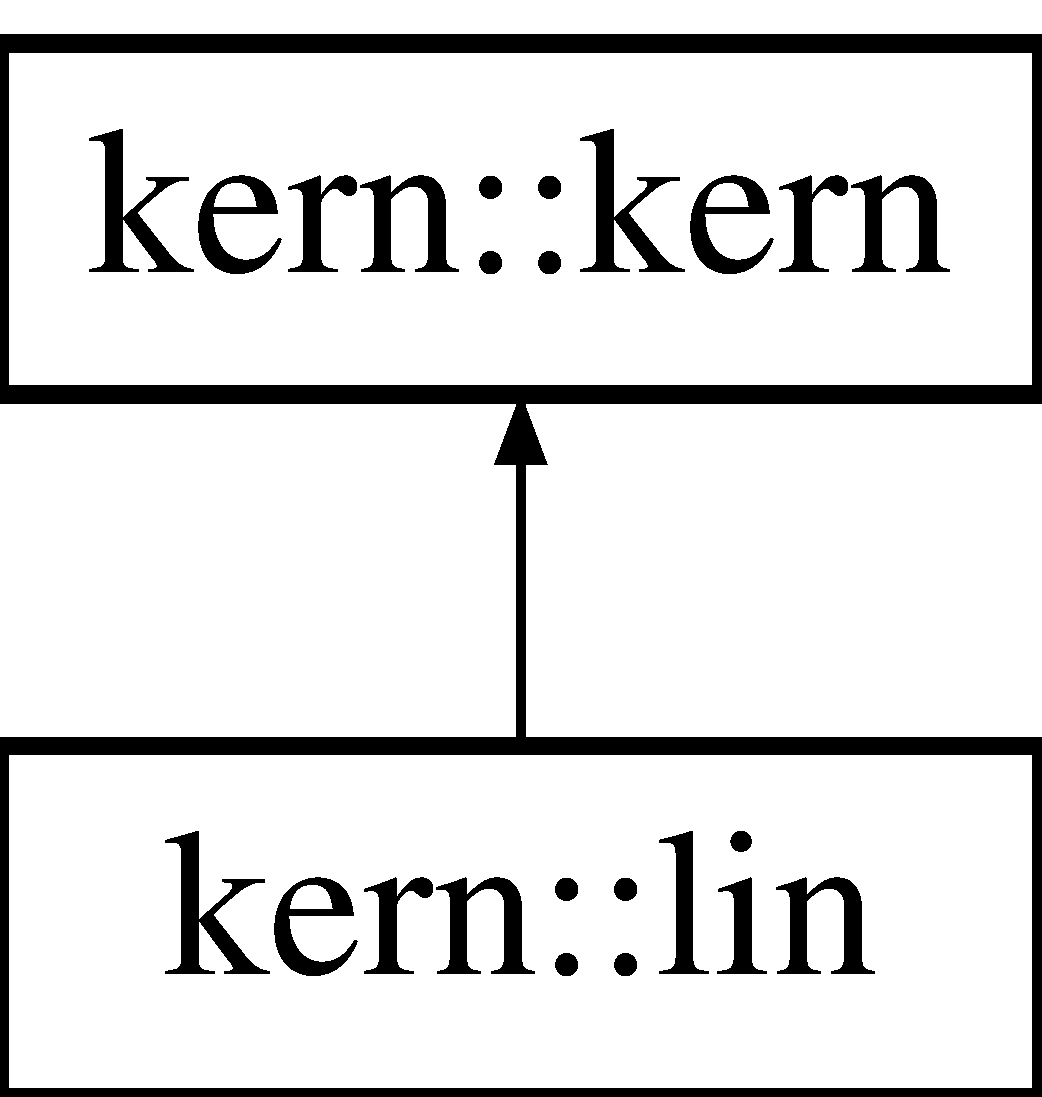
\includegraphics[height=2cm]{classkern_1_1lin}
\end{center}
\end{figure}
\subsection*{Public Member Functions}
\begin{CompactItemize}
\item 
\hypertarget{classkern_1_1lin_59909da6685c26988c716bf2c184a7f5}{
def \textbf{\_\-\_\-init\_\-\_\-}}
\label{classkern_1_1lin_59909da6685c26988c716bf2c184a7f5}

\item 
def \hyperlink{classkern_1_1lin_9eeb97cbc165d5825fdba59a45708c53}{paramInit}
\item 
def \hyperlink{classkern_1_1lin_38ca0676026a784df6529071fa572514}{compute}
\item 
def \hyperlink{classkern_1_1lin_006ba41a9245cb67da4a7d287b2423a5}{diagCompute}
\item 
def \hyperlink{classkern_1_1lin_e2f61ac06697bd58a4e8e58b43cbfa60}{diagGradX}
\item 
def \hyperlink{classkern_1_1lin_82e5c69d97b96f51a2dc32df91393aab}{diagGradient}
\item 
def \hyperlink{classkern_1_1lin_5f51f5aa6fb00f2435cf8a1d98b15ba1}{display}
\item 
def \hyperlink{classkern_1_1lin_52fab26598da0c88e64a63391d21255f}{expandParam}
\item 
def \hyperlink{classkern_1_1lin_c4f856301081962dd76ed1bc6a226c30}{extractParam}
\item 
def \hyperlink{classkern_1_1lin_5995d707a3fc482ed6c3abb1798e23a3}{extractParamNames}
\item 
def \hyperlink{classkern_1_1lin_ab69ae24e2845a8423f4fb12bae84198}{gradX}
\item 
def \hyperlink{classkern_1_1lin_383b1fe62ceac741d33759118cf30f3a}{gradient}
\end{CompactItemize}
\subsection*{Public Attributes}
\begin{CompactItemize}
\item 
\hypertarget{classkern_1_1lin_7b8c7bfd522d43511f45e7600f27d96a}{
\textbf{type}}
\label{classkern_1_1lin_7b8c7bfd522d43511f45e7600f27d96a}

\item 
\hypertarget{classkern_1_1lin_7dd1e0c7b4da8511fafb470561ef73c9}{
\textbf{variance}}
\label{classkern_1_1lin_7dd1e0c7b4da8511fafb470561ef73c9}

\item 
\hypertarget{classkern_1_1lin_b6cf32694074ab487cf883586ed9e21a}{
\textbf{nParams}}
\label{classkern_1_1lin_b6cf32694074ab487cf883586ed9e21a}

\item 
\hypertarget{classkern_1_1lin_5bfe56620dee043db851907a417ef8bb}{
\textbf{stationary}}
\label{classkern_1_1lin_5bfe56620dee043db851907a417ef8bb}

\item 
\hypertarget{classkern_1_1lin_5757cdc7b0312d33bd03db9c9164d65a}{
\textbf{normalised}}
\label{classkern_1_1lin_5757cdc7b0312d33bd03db9c9164d65a}

\end{CompactItemize}


\subsection{Detailed Description}


\footnotesize\begin{verbatim}% The linear kernel (LIN) is the simple inner product
% kernel. Sampling from this kernel produces linear functions.
%
% k(x_i, x_j) = sigma2 * x_i'*x_j
%
% There is one parameter, sigma2, which is stored in the field
% kern.variance.

\end{verbatim}
\normalsize
 

\subsection{Member Function Documentation}
\hypertarget{classkern_1_1lin_38ca0676026a784df6529071fa572514}{
\index{kern::lin@{kern::lin}!compute@{compute}}
\index{compute@{compute}!kern::lin@{kern::lin}}
\subsubsection[{compute}]{\setlength{\rightskip}{0pt plus 5cm}def kern::lin::compute ( {\em self}, \/   {\em x}, \/   {\em x2} = {\tt None})}}
\label{classkern_1_1lin_38ca0676026a784df6529071fa572514}




\footnotesize\begin{verbatim}% LINKERNCOMPUTE Compute the LIN kernel given the parameters and X.
% FORMAT
% DESC computes the kernel parameters for the linear
% kernel given inputs associated with rows and columns.
% ARG kern : the kernel structure for which the matrix is computed.
% ARG x : the input matrix associated with the rows of the kernel.
% ARG x2 : the input matrix associated with the columns of the kernel.
% RETURN k : the kernel matrix computed at the given points.
%
% FORMAT
% DESC computes the kernel matrix for the linear
% kernel given a design matrix of inputs.
% ARG kern : the kernel structure for which the matrix is computed.
% ARG x : input data matrix in the form of a design matrix.
% RETURN k : the kernel matrix computed at the given points.
%
% SEEALSO : linKernParamInit, kernCompute, kernCreate, linKernDiagCompute
%
% COPYRIGHT : Neil D. Lawrence, 2004, 2005, 2006, 2009

\end{verbatim}
\normalsize
 

Reimplemented from \hyperlink{classkern_1_1kern}{kern::kern}.\hypertarget{classkern_1_1lin_006ba41a9245cb67da4a7d287b2423a5}{
\index{kern::lin@{kern::lin}!diagCompute@{diagCompute}}
\index{diagCompute@{diagCompute}!kern::lin@{kern::lin}}
\subsubsection[{diagCompute}]{\setlength{\rightskip}{0pt plus 5cm}def kern::lin::diagCompute ( {\em self}, \/   {\em x})}}
\label{classkern_1_1lin_006ba41a9245cb67da4a7d287b2423a5}




\footnotesize\begin{verbatim}% LINKERNDIAGCOMPUTE Compute diagonal of LIN kernel.
% FORMAT
% DESC computes the diagonal of the kernel matrix for the linear kernel given a design matrix of inputs.
% ARG kern : the kernel structure for which the matrix is computed.
% ARG x : input data matrix in the form of a design matrix.
% RETURN k : a vector containing the diagonal of the kernel matrix
% computed at the given points.
%
% SEEALSO : linKernParamInit, kernDiagCompute, kernCreate, linKernCompute
%
% COPYRIGHT : Neil D. Lawrence, 2004, 2005, 2006, 2009

\end{verbatim}
\normalsize
 

Reimplemented from \hyperlink{classkern_1_1kern}{kern::kern}.\hypertarget{classkern_1_1lin_82e5c69d97b96f51a2dc32df91393aab}{
\index{kern::lin@{kern::lin}!diagGradient@{diagGradient}}
\index{diagGradient@{diagGradient}!kern::lin@{kern::lin}}
\subsubsection[{diagGradient}]{\setlength{\rightskip}{0pt plus 5cm}def kern::lin::diagGradient ( {\em self}, \/   {\em X}, \/   {\em covDiag})}}
\label{classkern_1_1lin_82e5c69d97b96f51a2dc32df91393aab}




\footnotesize\begin{verbatim}% DIAGGRADIENT Compute the gradient of the RBF kernel's diagonal wrt parameters.
% FORMAT
% DESC computes the gradient of functions of the diagonal of the
% radial basis function kernel matrix with respect to the parameters of the kernel. The
% parameters' gradients are returned in the order given by the
% rbfKernExtractParam command.
% ARG kern : the kernel structure for which the gradients are
% computed.
% ARG x : the input data for which the gradient is being computed.
% ARG factors : partial derivatives of the function of interest with
% respect to the diagonal elements of the kernel.
% RETURN g : gradients of the relevant function with respect to each
% of the parameters. Ordering should match the ordering given in
% rbfKernExtractParam.
%
% SEEALSO : gradient
%
% COPYRIGHT : Neil D. Lawrence, 2004-2006, 2009\end{verbatim}
\normalsize
 

Reimplemented from \hyperlink{classkern_1_1kern}{kern::kern}.\hypertarget{classkern_1_1lin_e2f61ac06697bd58a4e8e58b43cbfa60}{
\index{kern::lin@{kern::lin}!diagGradX@{diagGradX}}
\index{diagGradX@{diagGradX}!kern::lin@{kern::lin}}
\subsubsection[{diagGradX}]{\setlength{\rightskip}{0pt plus 5cm}def kern::lin::diagGradX ( {\em self}, \/   {\em X})}}
\label{classkern_1_1lin_e2f61ac06697bd58a4e8e58b43cbfa60}




\footnotesize\begin{verbatim}% LINKERNDIAGGRADX Gradient of LIN kernel's diagonal with respect to X.
% FORMAT
% DESC computes the gradient of the diagonal of the linear kernel matrix with
% respect to the elements of the design matrix given in X.
% ARG kern : the kernel structure for which gradients are being computed.
% ARG X : the input data in the form of a design matrix.
% RETURN gX : the gradients of the diagonal with respect to each element
% of X. The returned matrix has the same dimensions as X.
%
% SEEALSO : linKernParamInit, kernDiagGradX, linkernGradX
%
% COPYRIGHT : Neil D. Lawrence, 2004, 2005, 2006, 2009

\end{verbatim}
\normalsize
 

Reimplemented from \hyperlink{classkern_1_1kern}{kern::kern}.\hypertarget{classkern_1_1lin_5f51f5aa6fb00f2435cf8a1d98b15ba1}{
\index{kern::lin@{kern::lin}!display@{display}}
\index{display@{display}!kern::lin@{kern::lin}}
\subsubsection[{display}]{\setlength{\rightskip}{0pt plus 5cm}def kern::lin::display ( {\em self}, \/   {\em numSpaces} = {\tt 0})}}
\label{classkern_1_1lin_5f51f5aa6fb00f2435cf8a1d98b15ba1}




\footnotesize\begin{verbatim}% DISPLAY Display parameters of the LIN kernel.
% FORMAT
% DESC displays the parameters of the radial basis function
% kernel and the kernel type to the console.
% ARG kern : the kernel to display.
%
% FORMAT does the same as above, but indents the display according
% to the amount specified.
% ARG kern : the kernel to display.
% ARG spacing : how many spaces to indent the display of the kernel by.
%
% SEEALSO :
%
% COPYRIGHT : Neil D. Lawrence, 2004--2006, 2009

\end{verbatim}
\normalsize
 

Reimplemented from \hyperlink{classkern_1_1kern}{kern::kern}.\hypertarget{classkern_1_1lin_52fab26598da0c88e64a63391d21255f}{
\index{kern::lin@{kern::lin}!expandParam@{expandParam}}
\index{expandParam@{expandParam}!kern::lin@{kern::lin}}
\subsubsection[{expandParam}]{\setlength{\rightskip}{0pt plus 5cm}def kern::lin::expandParam ( {\em self}, \/   {\em params})}}
\label{classkern_1_1lin_52fab26598da0c88e64a63391d21255f}




\footnotesize\begin{verbatim}% EXPANDPARAM Create kernel structure from LIN kernel's parameters.
% FORMAT
% DESC returns a linear kernel structure filled with the
% parameters in the given vector. This is used as a helper function to
% enable parameters to be optimised in, for example, the NETLAB
% optimisation functions.
% ARG kern : the kernel structure in which the parameters are to be
% placed.
% ARG param : vector of parameters which are to be placed in the
% kernel structure.
% RETURN kern : kernel structure with the given parameters in the
% relevant locations.
%
% SEEALSO : extractParam
%
% COPYRIGHT : Neil D. Lawrence, 2004-2006, 2009\end{verbatim}
\normalsize
 \hypertarget{classkern_1_1lin_c4f856301081962dd76ed1bc6a226c30}{
\index{kern::lin@{kern::lin}!extractParam@{extractParam}}
\index{extractParam@{extractParam}!kern::lin@{kern::lin}}
\subsubsection[{extractParam}]{\setlength{\rightskip}{0pt plus 5cm}def kern::lin::extractParam ( {\em self})}}
\label{classkern_1_1lin_c4f856301081962dd76ed1bc6a226c30}




\footnotesize\begin{verbatim}% EXTRACTPARAM Extract parameters from the LIN kernel structure.
% FORMAT
% DESC Extract parameters from the linear kernel
% structure into a vector of parameters for optimisation.
% ARG kern : the kernel structure containing the parameters to be
% extracted.
% RETURN param : vector of parameters extracted from the kernel. If
% the field 'transforms' is not empty in the kernel matrix, the
% parameters will be transformed before optimisation (for example
% positive only parameters could be logged before being returned).
%
% SEEALSO expandParam, netlab.scg, netlab.conjgrad
%
% COPYRIGHT : Neil D. Lawrence, 2004--2006, 2009

\end{verbatim}
\normalsize
 \hypertarget{classkern_1_1lin_5995d707a3fc482ed6c3abb1798e23a3}{
\index{kern::lin@{kern::lin}!extractParamNames@{extractParamNames}}
\index{extractParamNames@{extractParamNames}!kern::lin@{kern::lin}}
\subsubsection[{extractParamNames}]{\setlength{\rightskip}{0pt plus 5cm}def kern::lin::extractParamNames ( {\em self})}}
\label{classkern_1_1lin_5995d707a3fc482ed6c3abb1798e23a3}




\footnotesize\begin{verbatim}% EXTRACTPARAMNAMES Extract parameter names from the LIN kernel structure.
% FORMAT
% DESC Extract parameter names from the linear kernel structure.
% ARG kern : the kernel structure containing the parameters to be
% extracted.
% RETURN names : cell array of strings giving names to the parameters.\end{verbatim}
\normalsize
 \hypertarget{classkern_1_1lin_383b1fe62ceac741d33759118cf30f3a}{
\index{kern::lin@{kern::lin}!gradient@{gradient}}
\index{gradient@{gradient}!kern::lin@{kern::lin}}
\subsubsection[{gradient}]{\setlength{\rightskip}{0pt plus 5cm}def kern::lin::gradient ( {\em self}, \/   {\em X}, \/   {\em X2} = {\tt None}, \/   {\em covGrad} = {\tt None})}}
\label{classkern_1_1lin_383b1fe62ceac741d33759118cf30f3a}




\footnotesize\begin{verbatim}% LINKERNGRADIENT Gradient of LIN kernel's parameters.
% FORMAT
% DESC computes the gradient of functions with respect to the
% linear
% kernel's parameters. As well as the kernel structure and the
% input positions, the user provides a matrix PARTIAL which gives
% the partial derivatives of the function with respect to the
% relevant elements of the kernel matrix. 
% ARG kern : the kernel structure for which the gradients are being
% computed.
% ARG x : the input locations for which the gradients are being
% computed. 
% ARG partial : matrix of partial derivatives of the function of
% interest with respect to the kernel matrix. The argument takes
% the form of a square matrix of dimension  numData, where numData is
% the number of rows in X.
% RETURN g : gradients of the function of interest with respect to
% the kernel parameters. The ordering of the vector should match
% that provided by the function kernExtractParam.
%
% FORMAT
% DESC computes the derivatives as above, but input locations are
% now provided in two matrices associated with rows and columns of
% the kernel matrix. 
% ARG kern : the kernel structure for which the gradients are being
% computed.
% ARG x1 : the input locations associated with the rows of the
% kernel matrix.
% ARG x2 : the input locations associated with the columns of the
% kernel matrix.
% ARG partial : matrix of partial derivatives of the function of
% interest with respect to the kernel matrix. The matrix should
% have the same number of rows as X1 and the same number of columns
% as X2 has rows.
% RETURN g : gradients of the function of interest with respect to
% the kernel parameters.
%
% SEEALSO linKernParamInit, kernGradient, linKernDiagGradient, kernGradX
%
% COPYRIGHT : Neil D. Lawrence, 2004, 2005, 2006, 2009

\end{verbatim}
\normalsize
 

Reimplemented from \hyperlink{classkern_1_1kern}{kern::kern}.\hypertarget{classkern_1_1lin_ab69ae24e2845a8423f4fb12bae84198}{
\index{kern::lin@{kern::lin}!gradX@{gradX}}
\index{gradX@{gradX}!kern::lin@{kern::lin}}
\subsubsection[{gradX}]{\setlength{\rightskip}{0pt plus 5cm}def kern::lin::gradX ( {\em self}, \/   {\em X}, \/   {\em X2})}}
\label{classkern_1_1lin_ab69ae24e2845a8423f4fb12bae84198}




\footnotesize\begin{verbatim}% GRADX Gradient of LIN kernel with respect to input locations.
% FORMAT
% DESC computes the gradient of the linear
% kernel with respect to the input positions where both the row
% positions and column positions are provided separately.
% ARG kern : kernel structure for which gradients are being
% computed.
% ARG x1 : row locations against which gradients are being computed.
% ARG x2 : column locations against which gradients are being computed.
% RETURN g : the returned gradients. The gradients are returned in
% a matrix which is numData2 x numInputs x numData1. Where numData1 is
% the number of data points in X1, numData2 is the number of data
% points in X2 and numInputs is the number of input
% dimensions in X.
%
% SEEALSO : diagGradX
%
% COPYRIGHT : Neil D. Lawrence, 2004-2006, 2009\end{verbatim}
\normalsize
 

Reimplemented from \hyperlink{classkern_1_1kern}{kern::kern}.\hypertarget{classkern_1_1lin_9eeb97cbc165d5825fdba59a45708c53}{
\index{kern::lin@{kern::lin}!paramInit@{paramInit}}
\index{paramInit@{paramInit}!kern::lin@{kern::lin}}
\subsubsection[{paramInit}]{\setlength{\rightskip}{0pt plus 5cm}def kern::lin::paramInit ( {\em self}, \/   {\em inDim} = {\tt None}, \/   {\em X} = {\tt None})}}
\label{classkern_1_1lin_9eeb97cbc165d5825fdba59a45708c53}




\footnotesize\begin{verbatim}% LINKERNPARAMINIT LIN kernel parameter initialisation.
% The linear kernel (LIN) is the simple inner product
% kernel. Sampling from this kernel produces linear functions.
%
% k(x_i, x_j) = sigma2 * x_i'*x_j
%
% There is one parameter, sigma2, which is stored in the field
% kern.variance.
%
% SEEALSO : linardKernParamInit
%
% FORMAT
% DESC initialises the linear
%  kernel structure with some default parameters.
% ARG kern : the kernel structure which requires initialisation.
% RETURN kern : the kernel structure with the default parameters placed in.
%
% SEEALSO : kernCreate, kernParamInit
%
% COPYRIGHT : Neil D. Lawrence, 2004, 2005, 2006, 2009

\end{verbatim}
\normalsize
 

The documentation for this class was generated from the following file:\begin{CompactItemize}
\item 
kern.py\end{CompactItemize}

\hypertarget{classkerndox_1_1lin}{
\section{kerndox::lin Class Reference}
\label{classkerndox_1_1lin}\index{kerndox::lin@{kerndox::lin}}
}
Inheritance diagram for kerndox::lin::\begin{figure}[H]
\begin{center}
\leavevmode
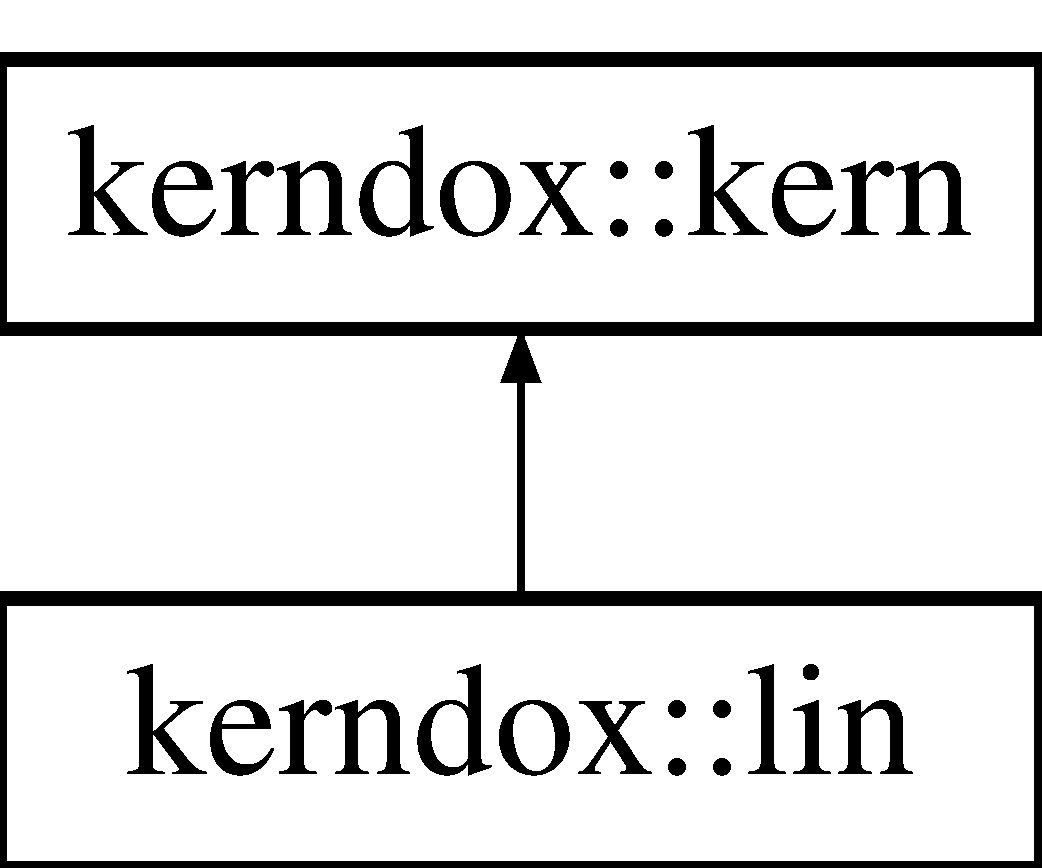
\includegraphics[height=2cm]{classkerndox_1_1lin}
\end{center}
\end{figure}
\subsection*{Public Member Functions}
\begin{CompactItemize}
\item 
\hypertarget{classkerndox_1_1lin_3ae2cb2e4dad731d71caac164caca68c}{
def \textbf{\_\-\_\-init\_\-\_\-}}
\label{classkerndox_1_1lin_3ae2cb2e4dad731d71caac164caca68c}

\item 
def \hyperlink{classkerndox_1_1lin_bb6282f0591600e43e8d0c14ddfa7ee5}{paramInit}
\item 
def \hyperlink{classkerndox_1_1lin_a44fb05c87a84233e7a8592b936debb1}{compute}
\item 
def \hyperlink{classkerndox_1_1lin_0031e74c9acb34a68479ade5f62aa8e3}{diagCompute}
\item 
def \hyperlink{classkerndox_1_1lin_8ea5c54102e2149052b7df6114f16102}{diagGradX}
\item 
def \hyperlink{classkerndox_1_1lin_a86845028577e7d1bed2496250d79d36}{diagGradient}
\item 
def \hyperlink{classkerndox_1_1lin_1920b7faa203c45f748c60a04f3e3493}{display}
\item 
def \hyperlink{classkerndox_1_1lin_1bd885c09b72a881bf508622e6081446}{expandParam}
\item 
def \hyperlink{classkerndox_1_1lin_7b932181554ce33a7f1cbbc3e916a074}{extractParam}
\item 
def \hyperlink{classkerndox_1_1lin_b9112aeafa2c481061e7fa517714ee7b}{extractParamNames}
\item 
def \hyperlink{classkerndox_1_1lin_6841d17e0033af3149d4627acc81fbfd}{gradX}
\item 
def \hyperlink{classkerndox_1_1lin_9681d3870e1bae2e62507c08f5868818}{gradient}
\end{CompactItemize}
\subsection*{Public Attributes}
\begin{CompactItemize}
\item 
\hypertarget{classkerndox_1_1lin_faaa9348303b8e71f462208b3de7000d}{
\textbf{type}}
\label{classkerndox_1_1lin_faaa9348303b8e71f462208b3de7000d}

\item 
\hypertarget{classkerndox_1_1lin_fcc4b138431f89cf9e32b12a4b37d0d3}{
\textbf{variance}}
\label{classkerndox_1_1lin_fcc4b138431f89cf9e32b12a4b37d0d3}

\item 
\hypertarget{classkerndox_1_1lin_50d3156549623f32b9ad60415304d3fc}{
\textbf{nParams}}
\label{classkerndox_1_1lin_50d3156549623f32b9ad60415304d3fc}

\item 
\hypertarget{classkerndox_1_1lin_04ec4ee0be6f50a9c371914a4abf1ffc}{
\textbf{stationary}}
\label{classkerndox_1_1lin_04ec4ee0be6f50a9c371914a4abf1ffc}

\item 
\hypertarget{classkerndox_1_1lin_6c60d32e29f376e3033e1728157da5fe}{
\textbf{normalised}}
\label{classkerndox_1_1lin_6c60d32e29f376e3033e1728157da5fe}

\end{CompactItemize}


\subsection{Detailed Description}


\footnotesize\begin{verbatim}The linear kernel (LIN) is the simple inner product
kernel. Sampling from this kernel produces linear functions.
%
k(x_i, x_j) = sigma2 * x_i'*x_j
%
There is one parameter, sigma2, which is stored in the field
kern.variance.

\end{verbatim}
\normalsize
 

\subsection{Member Function Documentation}
\hypertarget{classkerndox_1_1lin_a44fb05c87a84233e7a8592b936debb1}{
\index{kerndox::lin@{kerndox::lin}!compute@{compute}}
\index{compute@{compute}!kerndox::lin@{kerndox::lin}}
\subsubsection[{compute}]{\setlength{\rightskip}{0pt plus 5cm}def kerndox::lin::compute ( {\em self}, \/   {\em x}, \/   {\em x2} = {\tt None})}}
\label{classkerndox_1_1lin_a44fb05c87a84233e7a8592b936debb1}




\footnotesize\begin{verbatim}LINKERNCOMPUTE Compute the LIN kernel given the parameters and X.
FORMAT
DESC computes the kernel parameters for the linear
kernel given inputs associated with rows and columns.
\param kern : the kernel structure for which the matrix is computed.
\param x : the input matrix associated with the rows of the kernel.
\param x2 : the input matrix associated with the columns of the kernel.
\return  k : the kernel matrix computed at the given points.
%
FORMAT
DESC computes the kernel matrix for the linear
kernel given a design matrix of inputs.
\param kern : the kernel structure for which the matrix is computed.
\param x : input data matrix in the form of a design matrix.
\return  k : the kernel matrix computed at the given points.
%
SEEALSO : linKernParamInit, kernCompute, kernCreate, linKernDiagCompute
%
COPYRIGHT : Neil D. Lawrence, 2004, 2005, 2006, 2009

\end{verbatim}
\normalsize
 

Reimplemented from \hyperlink{classkerndox_1_1kern}{kerndox::kern}.\hypertarget{classkerndox_1_1lin_0031e74c9acb34a68479ade5f62aa8e3}{
\index{kerndox::lin@{kerndox::lin}!diagCompute@{diagCompute}}
\index{diagCompute@{diagCompute}!kerndox::lin@{kerndox::lin}}
\subsubsection[{diagCompute}]{\setlength{\rightskip}{0pt plus 5cm}def kerndox::lin::diagCompute ( {\em self}, \/   {\em x})}}
\label{classkerndox_1_1lin_0031e74c9acb34a68479ade5f62aa8e3}




\footnotesize\begin{verbatim}LINKERNDIAGCOMPUTE Compute diagonal of LIN kernel.
FORMAT
DESC computes the diagonal of the kernel matrix for the linear kernel given a design matrix of inputs.
\param kern : the kernel structure for which the matrix is computed.
\param x : input data matrix in the form of a design matrix.
\return  k : a vector containing the diagonal of the kernel matrix
computed at the given points.
%
SEEALSO : linKernParamInit, kernDiagCompute, kernCreate, linKernCompute
%
COPYRIGHT : Neil D. Lawrence, 2004, 2005, 2006, 2009

\end{verbatim}
\normalsize
 

Reimplemented from \hyperlink{classkerndox_1_1kern}{kerndox::kern}.\hypertarget{classkerndox_1_1lin_a86845028577e7d1bed2496250d79d36}{
\index{kerndox::lin@{kerndox::lin}!diagGradient@{diagGradient}}
\index{diagGradient@{diagGradient}!kerndox::lin@{kerndox::lin}}
\subsubsection[{diagGradient}]{\setlength{\rightskip}{0pt plus 5cm}def kerndox::lin::diagGradient ( {\em self}, \/   {\em X}, \/   {\em covDiag})}}
\label{classkerndox_1_1lin_a86845028577e7d1bed2496250d79d36}




\footnotesize\begin{verbatim}DIAGGRADIENT Compute the gradient of the RBF kernel's diagonal wrt parameters.
FORMAT
DESC computes the gradient of functions of the diagonal of the
radial basis function kernel matrix with respect to the parameters of the kernel. The
parameters' gradients are returned in the order given by the
rbfKernExtractParam command.
\param kern : the kernel structure for which the gradients are
computed.
\param x : the input data for which the gradient is being computed.
\param factors : partial derivatives of the function of interest with
respect to the diagonal elements of the kernel.
\return  g : gradients of the relevant function with respect to each
of the parameters. Ordering should match the ordering given in
rbfKernExtractParam.
%
SEEALSO : gradient
%
COPYRIGHT : Neil D. Lawrence, 2004-2006, 2009\end{verbatim}
\normalsize
 

Reimplemented from \hyperlink{classkerndox_1_1kern}{kerndox::kern}.\hypertarget{classkerndox_1_1lin_8ea5c54102e2149052b7df6114f16102}{
\index{kerndox::lin@{kerndox::lin}!diagGradX@{diagGradX}}
\index{diagGradX@{diagGradX}!kerndox::lin@{kerndox::lin}}
\subsubsection[{diagGradX}]{\setlength{\rightskip}{0pt plus 5cm}def kerndox::lin::diagGradX ( {\em self}, \/   {\em X})}}
\label{classkerndox_1_1lin_8ea5c54102e2149052b7df6114f16102}




\footnotesize\begin{verbatim}LINKERNDIAGGRADX Gradient of LIN kernel's diagonal with respect to X.
FORMAT
DESC computes the gradient of the diagonal of the linear kernel matrix with
respect to the elements of the design matrix given in X.
\param kern : the kernel structure for which gradients are being computed.
\param X : the input data in the form of a design matrix.
\return  gX : the gradients of the diagonal with respect to each element
of X. The returned matrix has the same dimensions as X.
%
SEEALSO : linKernParamInit, kernDiagGradX, linkernGradX
%
COPYRIGHT : Neil D. Lawrence, 2004, 2005, 2006, 2009

\end{verbatim}
\normalsize
 

Reimplemented from \hyperlink{classkerndox_1_1kern}{kerndox::kern}.\hypertarget{classkerndox_1_1lin_1920b7faa203c45f748c60a04f3e3493}{
\index{kerndox::lin@{kerndox::lin}!display@{display}}
\index{display@{display}!kerndox::lin@{kerndox::lin}}
\subsubsection[{display}]{\setlength{\rightskip}{0pt plus 5cm}def kerndox::lin::display ( {\em self}, \/   {\em numSpaces} = {\tt 0})}}
\label{classkerndox_1_1lin_1920b7faa203c45f748c60a04f3e3493}




\footnotesize\begin{verbatim}DISPLAY Display parameters of the LIN kernel.
FORMAT
DESC displays the parameters of the radial basis function
kernel and the kernel type to the console.
\param kern : the kernel to display.
%
FORMAT does the same as above, but indents the display according
to the amount specified.
\param kern : the kernel to display.
\param spacing : how many spaces to indent the display of the kernel by.
%
SEEALSO :
%
COPYRIGHT : Neil D. Lawrence, 2004--2006, 2009

\end{verbatim}
\normalsize
 

Reimplemented from \hyperlink{classkerndox_1_1kern}{kerndox::kern}.\hypertarget{classkerndox_1_1lin_1bd885c09b72a881bf508622e6081446}{
\index{kerndox::lin@{kerndox::lin}!expandParam@{expandParam}}
\index{expandParam@{expandParam}!kerndox::lin@{kerndox::lin}}
\subsubsection[{expandParam}]{\setlength{\rightskip}{0pt plus 5cm}def kerndox::lin::expandParam ( {\em self}, \/   {\em params})}}
\label{classkerndox_1_1lin_1bd885c09b72a881bf508622e6081446}




\footnotesize\begin{verbatim}EXPANDPARAM Create kernel structure from LIN kernel's parameters.
FORMAT
DESC returns a linear kernel structure filled with the
parameters in the given vector. This is used as a helper function to
enable parameters to be optimised in, for example, the NETLAB
optimisation functions.
\param kern : the kernel structure in which the parameters are to be
placed.
\param param : vector of parameters which are to be placed in the
kernel structure.
\return  kern : kernel structure with the given parameters in the
relevant locations.
%
SEEALSO : extractParam
%
COPYRIGHT : Neil D. Lawrence, 2004-2006, 2009\end{verbatim}
\normalsize
 \hypertarget{classkerndox_1_1lin_7b932181554ce33a7f1cbbc3e916a074}{
\index{kerndox::lin@{kerndox::lin}!extractParam@{extractParam}}
\index{extractParam@{extractParam}!kerndox::lin@{kerndox::lin}}
\subsubsection[{extractParam}]{\setlength{\rightskip}{0pt plus 5cm}def kerndox::lin::extractParam ( {\em self})}}
\label{classkerndox_1_1lin_7b932181554ce33a7f1cbbc3e916a074}




\footnotesize\begin{verbatim}EXTRACTPARAM Extract parameters from the LIN kernel structure.
FORMAT
DESC Extract parameters from the linear kernel
structure into a vector of parameters for optimisation.
\param kern : the kernel structure containing the parameters to be
extracted.
\return  param : vector of parameters extracted from the kernel. If
the field 'transforms' is not empty in the kernel matrix, the
parameters will be transformed before optimisation (for example
positive only parameters could be logged before being returned).
%
SEEALSO expandParam, netlab.scg, netlab.conjgrad
%
COPYRIGHT : Neil D. Lawrence, 2004--2006, 2009

\end{verbatim}
\normalsize
 \hypertarget{classkerndox_1_1lin_b9112aeafa2c481061e7fa517714ee7b}{
\index{kerndox::lin@{kerndox::lin}!extractParamNames@{extractParamNames}}
\index{extractParamNames@{extractParamNames}!kerndox::lin@{kerndox::lin}}
\subsubsection[{extractParamNames}]{\setlength{\rightskip}{0pt plus 5cm}def kerndox::lin::extractParamNames ( {\em self})}}
\label{classkerndox_1_1lin_b9112aeafa2c481061e7fa517714ee7b}




\footnotesize\begin{verbatim}EXTRACTPARAMNAMES Extract parameter names from the LIN kernel structure.
FORMAT
DESC Extract parameter names from the linear kernel structure.
\param kern : the kernel structure containing the parameters to be
extracted.
\return  names : cell array of strings giving names to the parameters.\end{verbatim}
\normalsize
 \hypertarget{classkerndox_1_1lin_9681d3870e1bae2e62507c08f5868818}{
\index{kerndox::lin@{kerndox::lin}!gradient@{gradient}}
\index{gradient@{gradient}!kerndox::lin@{kerndox::lin}}
\subsubsection[{gradient}]{\setlength{\rightskip}{0pt plus 5cm}def kerndox::lin::gradient ( {\em self}, \/   {\em X}, \/   {\em X2} = {\tt None}, \/   {\em covGrad} = {\tt None})}}
\label{classkerndox_1_1lin_9681d3870e1bae2e62507c08f5868818}




\footnotesize\begin{verbatim}LINKERNGRADIENT Gradient of LIN kernel's parameters.
FORMAT
DESC computes the gradient of functions with respect to the
linear
kernel's parameters. As well as the kernel structure and the
input positions, the user provides a matrix PARTIAL which gives
the partial derivatives of the function with respect to the
relevant elements of the kernel matrix. 
\param kern : the kernel structure for which the gradients are being
computed.
\param x : the input locations for which the gradients are being
computed. 
\param partial : matrix of partial derivatives of the function of
interest with respect to the kernel matrix. The argument takes
the form of a square matrix of dimension  numData, where numData is
the number of rows in X.
\return  g : gradients of the function of interest with respect to
the kernel parameters. The ordering of the vector should match
that provided by the function kernExtractParam.
%
FORMAT
DESC computes the derivatives as above, but input locations are
now provided in two matrices associated with rows and columns of
the kernel matrix. 
\param kern : the kernel structure for which the gradients are being
computed.
\param x1 : the input locations associated with the rows of the
kernel matrix.
\param x2 : the input locations associated with the columns of the
kernel matrix.
\param partial : matrix of partial derivatives of the function of
interest with respect to the kernel matrix. The matrix should
have the same number of rows as X1 and the same number of columns
as X2 has rows.
\return  g : gradients of the function of interest with respect to
the kernel parameters.
%
SEEALSO linKernParamInit, kernGradient, linKernDiagGradient, kernGradX
%
COPYRIGHT : Neil D. Lawrence, 2004, 2005, 2006, 2009

\end{verbatim}
\normalsize
 

Reimplemented from \hyperlink{classkerndox_1_1kern}{kerndox::kern}.\hypertarget{classkerndox_1_1lin_6841d17e0033af3149d4627acc81fbfd}{
\index{kerndox::lin@{kerndox::lin}!gradX@{gradX}}
\index{gradX@{gradX}!kerndox::lin@{kerndox::lin}}
\subsubsection[{gradX}]{\setlength{\rightskip}{0pt plus 5cm}def kerndox::lin::gradX ( {\em self}, \/   {\em X}, \/   {\em X2})}}
\label{classkerndox_1_1lin_6841d17e0033af3149d4627acc81fbfd}




\footnotesize\begin{verbatim}GRADX Gradient of LIN kernel with respect to input locations.
FORMAT
DESC computes the gradient of the linear
kernel with respect to the input positions where both the row
positions and column positions are provided separately.
\param kern : kernel structure for which gradients are being
computed.
\param x1 : row locations against which gradients are being computed.
\param x2 : column locations against which gradients are being computed.
\return  g : the returned gradients. The gradients are returned in
a matrix which is numData2 x numInputs x numData1. Where numData1 is
the number of data points in X1, numData2 is the number of data
points in X2 and numInputs is the number of input
dimensions in X.
%
SEEALSO : diagGradX
%
COPYRIGHT : Neil D. Lawrence, 2004-2006, 2009\end{verbatim}
\normalsize
 

Reimplemented from \hyperlink{classkerndox_1_1kern}{kerndox::kern}.\hypertarget{classkerndox_1_1lin_bb6282f0591600e43e8d0c14ddfa7ee5}{
\index{kerndox::lin@{kerndox::lin}!paramInit@{paramInit}}
\index{paramInit@{paramInit}!kerndox::lin@{kerndox::lin}}
\subsubsection[{paramInit}]{\setlength{\rightskip}{0pt plus 5cm}def kerndox::lin::paramInit ( {\em self}, \/   {\em inDim} = {\tt None}, \/   {\em X} = {\tt None})}}
\label{classkerndox_1_1lin_bb6282f0591600e43e8d0c14ddfa7ee5}




\footnotesize\begin{verbatim}LINKERNPARAMINIT LIN kernel parameter initialisation.
The linear kernel (LIN) is the simple inner product
kernel. Sampling from this kernel produces linear functions.
%
k(x_i, x_j) = sigma2 * x_i'*x_j
%
There is one parameter, sigma2, which is stored in the field
kern.variance.
%
SEEALSO : linardKernParamInit
%
FORMAT
DESC initialises the linear
 kernel structure with some default parameters.
\param kern : the kernel structure which requires initialisation.
\return  kern : the kernel structure with the default parameters placed in.
%
SEEALSO : kernCreate, kernParamInit
%
COPYRIGHT : Neil D. Lawrence, 2004, 2005, 2006, 2009

\end{verbatim}
\normalsize
 

The documentation for this class was generated from the following file:\begin{CompactItemize}
\item 
kerndox.py\end{CompactItemize}

\hypertarget{classkern_1_1rbf}{
\section{kern::rbf Class Reference}
\label{classkern_1_1rbf}\index{kern::rbf@{kern::rbf}}
}
Inheritance diagram for kern::rbf::\begin{figure}[H]
\begin{center}
\leavevmode
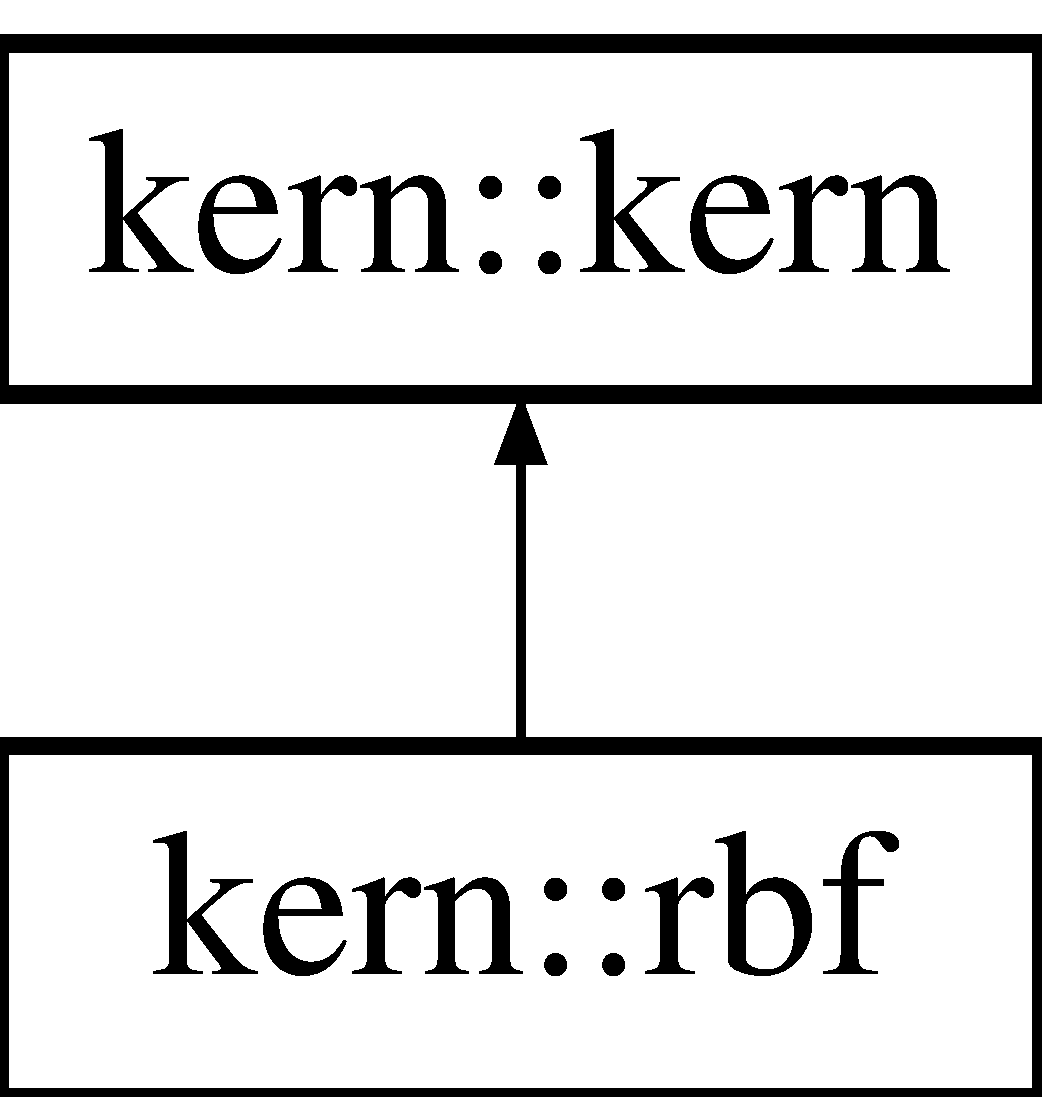
\includegraphics[height=2cm]{classkern_1_1rbf}
\end{center}
\end{figure}
\subsection*{Public Member Functions}
\begin{CompactItemize}
\item 
\hypertarget{classkern_1_1rbf_7ffa7cfcd57ac9cfeb73493edb813213}{
def \textbf{\_\-\_\-init\_\-\_\-}}
\label{classkern_1_1rbf_7ffa7cfcd57ac9cfeb73493edb813213}

\item 
def \hyperlink{classkern_1_1rbf_b027910bf4a6f9e6ca1b5cbaa0caae9e}{paramInit}
\item 
def \hyperlink{classkern_1_1rbf_be3823a7db917ca61725cb5083b0622b}{compute}
\item 
def \hyperlink{classkern_1_1rbf_5c3835b3bc757a209995a697670c972f}{diagCompute}
\item 
def \hyperlink{classkern_1_1rbf_eda4e0ee73de97348afe5ba685c6c8fe}{diagGradX}
\item 
def \hyperlink{classkern_1_1rbf_0bcf6593046cfb84aef5f9e19b8c5ab5}{diagGradient}
\item 
def \hyperlink{classkern_1_1rbf_20fdea38a18a1f81907c5a7d11d0eb22}{display}
\item 
def \hyperlink{classkern_1_1rbf_c514b52ff98203ead791b7f7a9c35469}{expandParam}
\item 
def \hyperlink{classkern_1_1rbf_bae71f49c71ee4a2f1c072e5262a8d07}{extractParam}
\item 
def \hyperlink{classkern_1_1rbf_612d8dca7710da14b51fd06e4cb52de4}{extractParamNames}
\item 
def \hyperlink{classkern_1_1rbf_8a5245cf870c42271886116e5e36281c}{gradX}
\item 
def \hyperlink{classkern_1_1rbf_c3778a9ca05e365081c672b370591558}{gradXpoint}
\item 
def \hyperlink{classkern_1_1rbf_baceff6cd7ac7bdc69d5797dff72c5d2}{gradient}
\end{CompactItemize}
\subsection*{Public Attributes}
\begin{CompactItemize}
\item 
\hypertarget{classkern_1_1rbf_b5215a71a9932013ae3919e0385aeee5}{
\textbf{type}}
\label{classkern_1_1rbf_b5215a71a9932013ae3919e0385aeee5}

\item 
\hypertarget{classkern_1_1rbf_d5a8729d56b374ebabcf17172235db08}{
\textbf{inverseWidth}}
\label{classkern_1_1rbf_d5a8729d56b374ebabcf17172235db08}

\item 
\hypertarget{classkern_1_1rbf_d6605302395ff7a395d1dcf4e905b6aa}{
\textbf{variance}}
\label{classkern_1_1rbf_d6605302395ff7a395d1dcf4e905b6aa}

\item 
\hypertarget{classkern_1_1rbf_27e852c7586f034079127ee44f53d7d4}{
\textbf{nParams}}
\label{classkern_1_1rbf_27e852c7586f034079127ee44f53d7d4}

\item 
\hypertarget{classkern_1_1rbf_54cd07c0448c54143b0bf58ddf47e8fb}{
\textbf{stationary}}
\label{classkern_1_1rbf_54cd07c0448c54143b0bf58ddf47e8fb}

\item 
\hypertarget{classkern_1_1rbf_167598c8831ddce0d7596e6ed2041b2f}{
\textbf{normalised}}
\label{classkern_1_1rbf_167598c8831ddce0d7596e6ed2041b2f}

\end{CompactItemize}


\subsection{Detailed Description}


\footnotesize\begin{verbatim}% The radial basis function kernel (RBF) is sometimes also known as
% the squared exponential kernel. It is a very smooth non-linear
% kernel and is a popular choice for generic use.
%
% k(x_i, x_j) = sigma2 * exp(-gamma/2 *(x_i - x_j)'*(x_i - x_j))
%
% The parameters are sigma2, the process variance (kern.variance)
% and gamma, the inverse width (kern.inverseWidth). The inverse
% width controls how wide the basis functions are, the larger
% gamma, the smaller the basis functions are.
%
% There is also an automatic relevance determination version of
% this kernel provided.

\end{verbatim}
\normalsize
 

\subsection{Member Function Documentation}
\hypertarget{classkern_1_1rbf_be3823a7db917ca61725cb5083b0622b}{
\index{kern::rbf@{kern::rbf}!compute@{compute}}
\index{compute@{compute}!kern::rbf@{kern::rbf}}
\subsubsection[{compute}]{\setlength{\rightskip}{0pt plus 5cm}def kern::rbf::compute ( {\em self}, \/   {\em x}, \/   {\em x2} = {\tt None})}}
\label{classkern_1_1rbf_be3823a7db917ca61725cb5083b0622b}




\footnotesize\begin{verbatim}% DESC computes the kernel parameters for the radial basis function
kernel given inputs associated with rows and columns.
% ARG kern : the kernel structure for which the matrix is computed.
% ARG x : the input matrix associated with the rows of the kernel.
% ARG x2 : the input matrix associated with the columns of the kernel.
% RETURN k : the kernel matrix computed at the given points.
 
% FORMAT
% DESC computes the kernel matrix for the radial basis function
kernel given a design matrix of inputs.
% ARG kern : the kernel structure for which the matrix is computed.
% ARG x : input data matrix in the form of a design matrix.
% RETURN k : the kernel matrix computed at the given points.
%
% SEEALSO : diagCompute
%
% COPYRIGHT : Neil D. Lawrence, 2004-2006, 2009

\end{verbatim}
\normalsize
 

Reimplemented from \hyperlink{classkern_1_1kern}{kern::kern}.\hypertarget{classkern_1_1rbf_5c3835b3bc757a209995a697670c972f}{
\index{kern::rbf@{kern::rbf}!diagCompute@{diagCompute}}
\index{diagCompute@{diagCompute}!kern::rbf@{kern::rbf}}
\subsubsection[{diagCompute}]{\setlength{\rightskip}{0pt plus 5cm}def kern::rbf::diagCompute ( {\em self}, \/   {\em x})}}
\label{classkern_1_1rbf_5c3835b3bc757a209995a697670c972f}




\footnotesize\begin{verbatim}% DIAGCOMPUTE Compute diagonal of RBF kernel.
% FORMAT
% DESC computes the diagonal of the kernel matrix for the radial basis function kernel given a design matrix of inputs.
% ARG kern : the kernel structure for which the matrix is computed.
% ARG x : input data matrix in the form of a design matrix.
% RETURN k : a vector containing the diagonal of the kernel matrix
% computed at the given points.
%
% SEEALSO : compute
%
% COPYRIGHT : Neil D. Lawrence, 2004, 2005, 2006

\end{verbatim}
\normalsize
 

Reimplemented from \hyperlink{classkern_1_1kern}{kern::kern}.\hypertarget{classkern_1_1rbf_0bcf6593046cfb84aef5f9e19b8c5ab5}{
\index{kern::rbf@{kern::rbf}!diagGradient@{diagGradient}}
\index{diagGradient@{diagGradient}!kern::rbf@{kern::rbf}}
\subsubsection[{diagGradient}]{\setlength{\rightskip}{0pt plus 5cm}def kern::rbf::diagGradient ( {\em self}, \/   {\em X}, \/   {\em covDiag})}}
\label{classkern_1_1rbf_0bcf6593046cfb84aef5f9e19b8c5ab5}




\footnotesize\begin{verbatim}% DIAGGRADIENT Compute the gradient of the RBF kernel's diagonal wrt parameters.
% FORMAT
% DESC computes the gradient of functions of the diagonal of the
% radial basis function kernel matrix with respect to the parameters of the kernel. The
% parameters' gradients are returned in the order given by the
% rbfKernExtractParam command.
% ARG kern : the kernel structure for which the gradients are
% computed.
% ARG x : the input data for which the gradient is being computed.
% ARG factors : partial derivatives of the function of interest with
% respect to the diagonal elements of the kernel.
% RETURN g : gradients of the relevant function with respect to each
% of the parameters. Ordering should match the ordering given in
% rbfKernExtractParam.
%
% SEEALSO : gradient
%
% COPYRIGHT : Neil D. Lawrence, 2004-2006, 2009

\end{verbatim}
\normalsize
 

Reimplemented from \hyperlink{classkern_1_1kern}{kern::kern}.\hypertarget{classkern_1_1rbf_eda4e0ee73de97348afe5ba685c6c8fe}{
\index{kern::rbf@{kern::rbf}!diagGradX@{diagGradX}}
\index{diagGradX@{diagGradX}!kern::rbf@{kern::rbf}}
\subsubsection[{diagGradX}]{\setlength{\rightskip}{0pt plus 5cm}def kern::rbf::diagGradX ( {\em self}, \/   {\em X})}}
\label{classkern_1_1rbf_eda4e0ee73de97348afe5ba685c6c8fe}




\footnotesize\begin{verbatim}% DIAGGRADX Gradient of RBF kernel's diagonal with respect to X.
% FORMAT
% DESC computes the gradient of the diagonal of the radial basis function kernel matrix with
% respect to the elements of the design matrix given in X.
% ARG kern : the kernel structure for which gradients are being computed.
% ARG X : the input data in the form of a design matrix.
% RETURN gX : the gradients of the diagonal with respect to each element
% of X. The returned matrix has the same dimensions as X.
%
% SEEALSO : gradX
%
% COPYRIGHT : Neil D. Lawrence, 2004--2006, 2009

\end{verbatim}
\normalsize
 

Reimplemented from \hyperlink{classkern_1_1kern}{kern::kern}.\hypertarget{classkern_1_1rbf_20fdea38a18a1f81907c5a7d11d0eb22}{
\index{kern::rbf@{kern::rbf}!display@{display}}
\index{display@{display}!kern::rbf@{kern::rbf}}
\subsubsection[{display}]{\setlength{\rightskip}{0pt plus 5cm}def kern::rbf::display ( {\em self}, \/   {\em numSpaces} = {\tt 0})}}
\label{classkern_1_1rbf_20fdea38a18a1f81907c5a7d11d0eb22}




\footnotesize\begin{verbatim}% DISPLAY Display parameters of the RBF kernel.
% FORMAT
% DESC displays the parameters of the radial basis function
% kernel and the kernel type to the console.
% ARG kern : the kernel to display.
%
% FORMAT does the same as above, but indents the display according
% to the amount specified.
% ARG kern : the kernel to display.
% ARG spacing : how many spaces to indent the display of the kernel by.
%
% SEEALSO :
%
% COPYRIGHT : Neil D. Lawrence, 2004--2006, 2009

\end{verbatim}
\normalsize
 

Reimplemented from \hyperlink{classkern_1_1kern}{kern::kern}.\hypertarget{classkern_1_1rbf_c514b52ff98203ead791b7f7a9c35469}{
\index{kern::rbf@{kern::rbf}!expandParam@{expandParam}}
\index{expandParam@{expandParam}!kern::rbf@{kern::rbf}}
\subsubsection[{expandParam}]{\setlength{\rightskip}{0pt plus 5cm}def kern::rbf::expandParam ( {\em self}, \/   {\em params})}}
\label{classkern_1_1rbf_c514b52ff98203ead791b7f7a9c35469}




\footnotesize\begin{verbatim}% EXPANDPARAM Create kernel structure from RBF kernel's parameters.
% FORMAT
% DESC returns a radial basis function kernel structure filled with the
% parameters in the given vector. This is used as a helper function to
% enable parameters to be optimised in, for example, the NETLAB
% optimisation functions.
% ARG kern : the kernel structure in which the parameters are to be
% placed.
% ARG param : vector of parameters which are to be placed in the
% kernel structure.
% RETURN kern : kernel structure with the given parameters in the
% relevant locations.
%
% SEEALSO : extractParam
%
% COPYRIGHT : Neil D. Lawrence, 2004-2006, 2009

\end{verbatim}
\normalsize
 \hypertarget{classkern_1_1rbf_bae71f49c71ee4a2f1c072e5262a8d07}{
\index{kern::rbf@{kern::rbf}!extractParam@{extractParam}}
\index{extractParam@{extractParam}!kern::rbf@{kern::rbf}}
\subsubsection[{extractParam}]{\setlength{\rightskip}{0pt plus 5cm}def kern::rbf::extractParam ( {\em self})}}
\label{classkern_1_1rbf_bae71f49c71ee4a2f1c072e5262a8d07}




\footnotesize\begin{verbatim}% EXTRACTPARAM Extract parameters from the RBF kernel structure.
% FORMAT
% DESC Extract parameters from the radial basis function kernel
% structure into a vector of parameters for optimisation.
% ARG kern : the kernel structure containing the parameters to be
% extracted.
% RETURN param : vector of parameters extracted from the kernel. If
% the field 'transforms' is not empty in the kernel matrix, the
% parameters will be transformed before optimisation (for example
% positive only parameters could be logged before being returned).
%
% SEEALSO expandParam, netlab.scg, netlab.conjgrad
%
% COPYRIGHT : Neil D. Lawrence, 2004--2006, 2009

\end{verbatim}
\normalsize
 \hypertarget{classkern_1_1rbf_612d8dca7710da14b51fd06e4cb52de4}{
\index{kern::rbf@{kern::rbf}!extractParamNames@{extractParamNames}}
\index{extractParamNames@{extractParamNames}!kern::rbf@{kern::rbf}}
\subsubsection[{extractParamNames}]{\setlength{\rightskip}{0pt plus 5cm}def kern::rbf::extractParamNames ( {\em self})}}
\label{classkern_1_1rbf_612d8dca7710da14b51fd06e4cb52de4}




\footnotesize\begin{verbatim}% EXTRACTPARAMNAMES Extract parameter names from the RBF kernel structure.
% FORMAT
% DESC Extract parameter names from the radial basis
% function kernel structure.
% ARG kern : the kernel structure containing the parameters to be
% extracted.
% RETURN names : cell array of strings giving names to the parameters.

\end{verbatim}
\normalsize
 \hypertarget{classkern_1_1rbf_baceff6cd7ac7bdc69d5797dff72c5d2}{
\index{kern::rbf@{kern::rbf}!gradient@{gradient}}
\index{gradient@{gradient}!kern::rbf@{kern::rbf}}
\subsubsection[{gradient}]{\setlength{\rightskip}{0pt plus 5cm}def kern::rbf::gradient ( {\em self}, \/   {\em X}, \/   {\em X2} = {\tt None}, \/   {\em covGrad} = {\tt None})}}
\label{classkern_1_1rbf_baceff6cd7ac7bdc69d5797dff72c5d2}




\footnotesize\begin{verbatim}% GRADIENT Gradient of RBF kernel's parameters.
% FORMAT
% DESC computes the gradient of functions with respect to the
% radial basis function
% kernel's parameters. As well as the kernel structure and the
% input positions, the user provides a matrix PARTIAL which gives
% the partial derivatives of the function with respect to the
% relevant elements of the kernel matrix. 
% ARG kern : the kernel structure for which the gradients are being
% computed.
% ARG x : the input locations for which the gradients are being
% computed. 
% ARG partial : matrix of partial derivatives of the function of
% interest with respect to the kernel matrix. The argument takes
% the form of a square matrix of dimension  numData, where numData is
% the number of rows in X.
% RETURN g : gradients of the function of interest with respect to
% the kernel parameters. The ordering of the vector should match
% that provided by the function extractParam.
%
% FORMAT
% DESC computes the derivatives as above, but input locations are
% now provided in two matrices associated with rows and columns of
% the kernel matrix. 
% ARG kern : the kernel structure for which the gradients are being
% computed.
% ARG x1 : the input locations associated with the rows of the
% kernel matrix.
% ARG x2 : the input locations associated with the columns of the
% kernel matrix.
% ARG partial : matrix of partial derivatives of the function of
% interest with respect to the kernel matrix. The matrix should
% have the same number of rows as X1 and the same number of columns
% as X2 has rows.
% RETURN g : gradients of the function of interest with respect to
% the kernel parameters.
%
% SEEALSO diagGradient, gradX
%
% COPYRIGHT : Neil D. Lawrence, 2004-2006, 2009

\end{verbatim}
\normalsize
 

Reimplemented from \hyperlink{classkern_1_1kern}{kern::kern}.\hypertarget{classkern_1_1rbf_8a5245cf870c42271886116e5e36281c}{
\index{kern::rbf@{kern::rbf}!gradX@{gradX}}
\index{gradX@{gradX}!kern::rbf@{kern::rbf}}
\subsubsection[{gradX}]{\setlength{\rightskip}{0pt plus 5cm}def kern::rbf::gradX ( {\em self}, \/   {\em X}, \/   {\em X2})}}
\label{classkern_1_1rbf_8a5245cf870c42271886116e5e36281c}




\footnotesize\begin{verbatim}% GRADX Gradient of RBF kernel with respect to input locations.
% FORMAT
% DESC computes the gradident of the radial basis function
% kernel with respect to the input positions where both the row
% positions and column positions are provided separately.
% ARG kern : kernel structure for which gradients are being
% computed.
% ARG x1 : row locations against which gradients are being computed.
% ARG x2 : column locations against which gradients are being computed.
% RETURN g : the returned gradients. The gradients are returned in
% a matrix which is numData2 x numInputs x numData1. Where numData1 is
% the number of data points in X1, numData2 is the number of data
% points in X2 and numInputs is the number of input
% dimensions in X.
%
% SEEALSO : diagGradX
%
% COPYRIGHT : Neil D. Lawrence, 2004-2006, 2009

\end{verbatim}
\normalsize
 

Reimplemented from \hyperlink{classkern_1_1kern}{kern::kern}.\hypertarget{classkern_1_1rbf_c3778a9ca05e365081c672b370591558}{
\index{kern::rbf@{kern::rbf}!gradXpoint@{gradXpoint}}
\index{gradXpoint@{gradXpoint}!kern::rbf@{kern::rbf}}
\subsubsection[{gradXpoint}]{\setlength{\rightskip}{0pt plus 5cm}def kern::rbf::gradXpoint ( {\em self}, \/   {\em x}, \/   {\em X2})}}
\label{classkern_1_1rbf_c3778a9ca05e365081c672b370591558}




\footnotesize\begin{verbatim}% GRADXPOINT Gradient with respect to one point of x.\end{verbatim}
\normalsize
 \hypertarget{classkern_1_1rbf_b027910bf4a6f9e6ca1b5cbaa0caae9e}{
\index{kern::rbf@{kern::rbf}!paramInit@{paramInit}}
\index{paramInit@{paramInit}!kern::rbf@{kern::rbf}}
\subsubsection[{paramInit}]{\setlength{\rightskip}{0pt plus 5cm}def kern::rbf::paramInit ( {\em self}, \/   {\em inDim} = {\tt None}, \/   {\em X} = {\tt None})}}
\label{classkern_1_1rbf_b027910bf4a6f9e6ca1b5cbaa0caae9e}




\footnotesize\begin{verbatim}% RBFKERNPARAMINIT RBF kernel parameter initialisation.
%
% SEEALSO : rbfardKernParamInit
%
% FORMAT
% DESC initialises the radial basis function
%  kernel structure with some default parameters.
% ARG kern : the kernel structure which requires initialisation.
% RETURN kern : the kernel structure with the default parameters placed in.
%
% SEEALSO : create, kernParamInit
%
% COPYRIGHT : Neil D. Lawrence, 2004, 2005, 2006

\end{verbatim}
\normalsize
 

The documentation for this class was generated from the following file:\begin{CompactItemize}
\item 
kern.py\end{CompactItemize}

\hypertarget{classkerndox_1_1rbf}{
\section{kerndox::rbf Class Reference}
\label{classkerndox_1_1rbf}\index{kerndox::rbf@{kerndox::rbf}}
}
Inheritance diagram for kerndox::rbf::\begin{figure}[H]
\begin{center}
\leavevmode
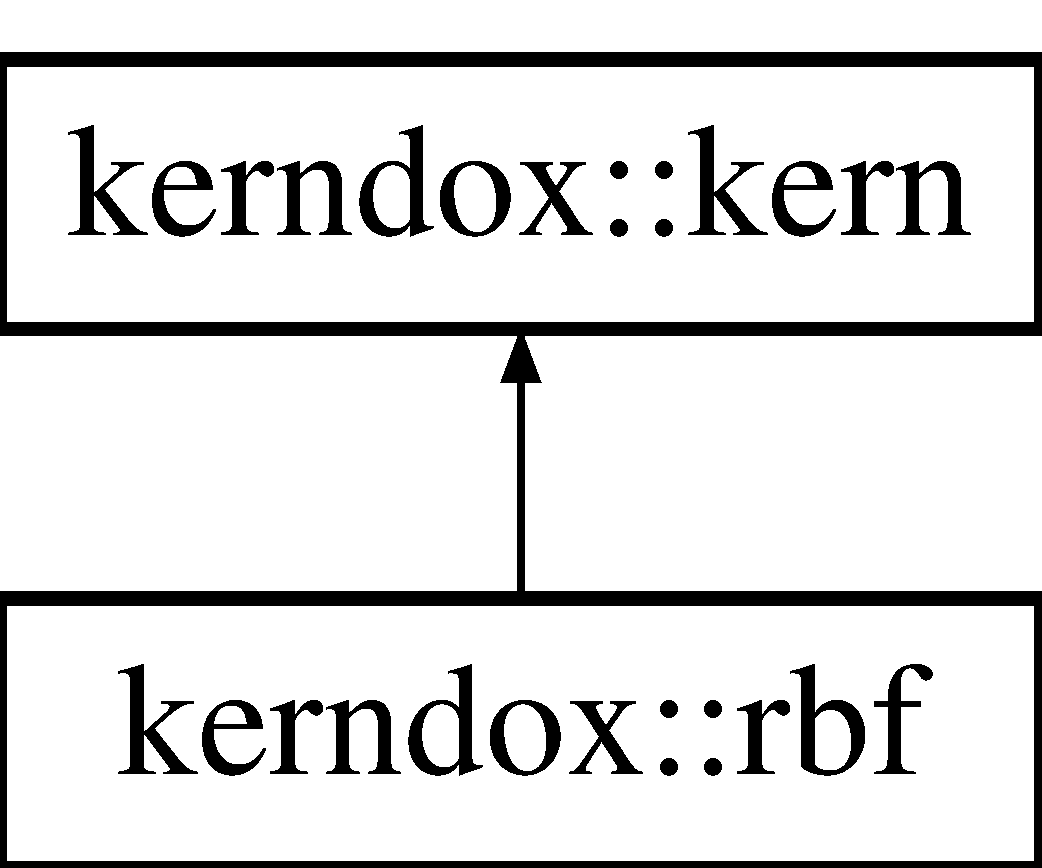
\includegraphics[height=2cm]{classkerndox_1_1rbf}
\end{center}
\end{figure}
\subsection*{Public Member Functions}
\begin{CompactItemize}
\item 
\hypertarget{classkerndox_1_1rbf_7bef5ec030e5f2f6688036046fd1baf4}{
def \textbf{\_\-\_\-init\_\-\_\-}}
\label{classkerndox_1_1rbf_7bef5ec030e5f2f6688036046fd1baf4}

\item 
def \hyperlink{classkerndox_1_1rbf_f1bacaa66cb4060943170900db397ea6}{paramInit}
\item 
def \hyperlink{classkerndox_1_1rbf_a041cf766fdfa3d3ddd373171e9b7d76}{compute}
\item 
def \hyperlink{classkerndox_1_1rbf_b29662ffe6791729f8e671a62e0a84b9}{diagCompute}
\item 
def \hyperlink{classkerndox_1_1rbf_ecdf6a3ae961ea26d9cc102767d93795}{diagGradX}
\item 
def \hyperlink{classkerndox_1_1rbf_8b5c3e33cf0ccc24afe05d49136d428a}{diagGradient}
\item 
def \hyperlink{classkerndox_1_1rbf_3559f5ba5512e4aa8a602dad0fa941fc}{display}
\item 
def \hyperlink{classkerndox_1_1rbf_847349971e97766b4fe4db1d4083708c}{expandParam}
\item 
def \hyperlink{classkerndox_1_1rbf_a81e44bc54a3442798c96bda3b3fd197}{extractParam}
\item 
def \hyperlink{classkerndox_1_1rbf_9e5c81421d3c9e23bd3d5341c15c08db}{extractParamNames}
\item 
def \hyperlink{classkerndox_1_1rbf_d7293550322f0cb3a5b97f2dea290318}{gradX}
\item 
def \hyperlink{classkerndox_1_1rbf_955b1766431cae06569e98329afb77bc}{gradXpoint}
\item 
def \hyperlink{classkerndox_1_1rbf_5cbf99c41f037ab3982c8595036ff205}{gradient}
\end{CompactItemize}
\subsection*{Public Attributes}
\begin{CompactItemize}
\item 
\hypertarget{classkerndox_1_1rbf_93974cc6c6fd731226b7c08aefbc9535}{
\textbf{type}}
\label{classkerndox_1_1rbf_93974cc6c6fd731226b7c08aefbc9535}

\item 
\hypertarget{classkerndox_1_1rbf_f5afeb1b2bde9987fdfbc5f1d0feea5c}{
\textbf{inverseWidth}}
\label{classkerndox_1_1rbf_f5afeb1b2bde9987fdfbc5f1d0feea5c}

\item 
\hypertarget{classkerndox_1_1rbf_f1c9cf8859b45fc4e0c79de0b7bcd273}{
\textbf{variance}}
\label{classkerndox_1_1rbf_f1c9cf8859b45fc4e0c79de0b7bcd273}

\item 
\hypertarget{classkerndox_1_1rbf_09bc0ec13a8c7ecccbb49e37aa92537d}{
\textbf{nParams}}
\label{classkerndox_1_1rbf_09bc0ec13a8c7ecccbb49e37aa92537d}

\item 
\hypertarget{classkerndox_1_1rbf_08289a7c641d13fdabc7463d39b0992d}{
\textbf{stationary}}
\label{classkerndox_1_1rbf_08289a7c641d13fdabc7463d39b0992d}

\item 
\hypertarget{classkerndox_1_1rbf_05ff5e0809d631804cd2f73b95694a78}{
\textbf{normalised}}
\label{classkerndox_1_1rbf_05ff5e0809d631804cd2f73b95694a78}

\end{CompactItemize}


\subsection{Detailed Description}


\footnotesize\begin{verbatim}The radial basis function kernel (RBF) is sometimes also known as
the squared exponential kernel. It is a very smooth non-linear
kernel and is a popular choice for generic use.
%
k(x_i, x_j) = sigma2 * exp(-gamma/2 *(x_i - x_j)'*(x_i - x_j))
%
The parameters are sigma2, the process variance (kern.variance)
and gamma, the inverse width (kern.inverseWidth). The inverse
width controls how wide the basis functions are, the larger
gamma, the smaller the basis functions are.
%
There is also an automatic relevance determination version of
this kernel provided.

\end{verbatim}
\normalsize
 

\subsection{Member Function Documentation}
\hypertarget{classkerndox_1_1rbf_a041cf766fdfa3d3ddd373171e9b7d76}{
\index{kerndox::rbf@{kerndox::rbf}!compute@{compute}}
\index{compute@{compute}!kerndox::rbf@{kerndox::rbf}}
\subsubsection[{compute}]{\setlength{\rightskip}{0pt plus 5cm}def kerndox::rbf::compute ( {\em self}, \/   {\em x}, \/   {\em x2} = {\tt None})}}
\label{classkerndox_1_1rbf_a041cf766fdfa3d3ddd373171e9b7d76}




\footnotesize\begin{verbatim}DESC computes the kernel parameters for the radial basis function
kernel given inputs associated with rows and columns.
\param kern : the kernel structure for which the matrix is computed.
\param x : the input matrix associated with the rows of the kernel.
\param x2 : the input matrix associated with the columns of the kernel.
\return  k : the kernel matrix computed at the given points.
 
FORMAT
DESC computes the kernel matrix for the radial basis function
kernel given a design matrix of inputs.
\param kern : the kernel structure for which the matrix is computed.
\param x : input data matrix in the form of a design matrix.
\return  k : the kernel matrix computed at the given points.
%
SEEALSO : diagCompute
%
COPYRIGHT : Neil D. Lawrence, 2004-2006, 2009

\end{verbatim}
\normalsize
 

Reimplemented from \hyperlink{classkerndox_1_1kern}{kerndox::kern}.\hypertarget{classkerndox_1_1rbf_b29662ffe6791729f8e671a62e0a84b9}{
\index{kerndox::rbf@{kerndox::rbf}!diagCompute@{diagCompute}}
\index{diagCompute@{diagCompute}!kerndox::rbf@{kerndox::rbf}}
\subsubsection[{diagCompute}]{\setlength{\rightskip}{0pt plus 5cm}def kerndox::rbf::diagCompute ( {\em self}, \/   {\em x})}}
\label{classkerndox_1_1rbf_b29662ffe6791729f8e671a62e0a84b9}




\footnotesize\begin{verbatim}DIAGCOMPUTE Compute diagonal of RBF kernel.
FORMAT
DESC computes the diagonal of the kernel matrix for the radial basis function kernel given a design matrix of inputs.
\param kern : the kernel structure for which the matrix is computed.
\param x : input data matrix in the form of a design matrix.
\return  k : a vector containing the diagonal of the kernel matrix
computed at the given points.
%
SEEALSO : compute
%
COPYRIGHT : Neil D. Lawrence, 2004, 2005, 2006

\end{verbatim}
\normalsize
 

Reimplemented from \hyperlink{classkerndox_1_1kern}{kerndox::kern}.\hypertarget{classkerndox_1_1rbf_8b5c3e33cf0ccc24afe05d49136d428a}{
\index{kerndox::rbf@{kerndox::rbf}!diagGradient@{diagGradient}}
\index{diagGradient@{diagGradient}!kerndox::rbf@{kerndox::rbf}}
\subsubsection[{diagGradient}]{\setlength{\rightskip}{0pt plus 5cm}def kerndox::rbf::diagGradient ( {\em self}, \/   {\em X}, \/   {\em covDiag})}}
\label{classkerndox_1_1rbf_8b5c3e33cf0ccc24afe05d49136d428a}




\footnotesize\begin{verbatim}DIAGGRADIENT Compute the gradient of the RBF kernel's diagonal wrt parameters.
FORMAT
DESC computes the gradient of functions of the diagonal of the
radial basis function kernel matrix with respect to the parameters of the kernel. The
parameters' gradients are returned in the order given by the
rbfKernExtractParam command.
\param kern : the kernel structure for which the gradients are
computed.
\param x : the input data for which the gradient is being computed.
\param factors : partial derivatives of the function of interest with
respect to the diagonal elements of the kernel.
\return  g : gradients of the relevant function with respect to each
of the parameters. Ordering should match the ordering given in
rbfKernExtractParam.
%
SEEALSO : gradient
%
COPYRIGHT : Neil D. Lawrence, 2004-2006, 2009

\end{verbatim}
\normalsize
 

Reimplemented from \hyperlink{classkerndox_1_1kern}{kerndox::kern}.\hypertarget{classkerndox_1_1rbf_ecdf6a3ae961ea26d9cc102767d93795}{
\index{kerndox::rbf@{kerndox::rbf}!diagGradX@{diagGradX}}
\index{diagGradX@{diagGradX}!kerndox::rbf@{kerndox::rbf}}
\subsubsection[{diagGradX}]{\setlength{\rightskip}{0pt plus 5cm}def kerndox::rbf::diagGradX ( {\em self}, \/   {\em X})}}
\label{classkerndox_1_1rbf_ecdf6a3ae961ea26d9cc102767d93795}




\footnotesize\begin{verbatim}DIAGGRADX Gradient of RBF kernel's diagonal with respect to X.
FORMAT
DESC computes the gradient of the diagonal of the radial basis function kernel matrix with
respect to the elements of the design matrix given in X.
\param kern : the kernel structure for which gradients are being computed.
\param X : the input data in the form of a design matrix.
\return  gX : the gradients of the diagonal with respect to each element
of X. The returned matrix has the same dimensions as X.
%
SEEALSO : gradX
%
COPYRIGHT : Neil D. Lawrence, 2004--2006, 2009

\end{verbatim}
\normalsize
 

Reimplemented from \hyperlink{classkerndox_1_1kern}{kerndox::kern}.\hypertarget{classkerndox_1_1rbf_3559f5ba5512e4aa8a602dad0fa941fc}{
\index{kerndox::rbf@{kerndox::rbf}!display@{display}}
\index{display@{display}!kerndox::rbf@{kerndox::rbf}}
\subsubsection[{display}]{\setlength{\rightskip}{0pt plus 5cm}def kerndox::rbf::display ( {\em self}, \/   {\em numSpaces} = {\tt 0})}}
\label{classkerndox_1_1rbf_3559f5ba5512e4aa8a602dad0fa941fc}




\footnotesize\begin{verbatim}DISPLAY Display parameters of the RBF kernel.
FORMAT
DESC displays the parameters of the radial basis function
kernel and the kernel type to the console.
\param kern : the kernel to display.
%
FORMAT does the same as above, but indents the display according
to the amount specified.
\param kern : the kernel to display.
\param spacing : how many spaces to indent the display of the kernel by.
%
SEEALSO :
%
COPYRIGHT : Neil D. Lawrence, 2004--2006, 2009

\end{verbatim}
\normalsize
 

Reimplemented from \hyperlink{classkerndox_1_1kern}{kerndox::kern}.\hypertarget{classkerndox_1_1rbf_847349971e97766b4fe4db1d4083708c}{
\index{kerndox::rbf@{kerndox::rbf}!expandParam@{expandParam}}
\index{expandParam@{expandParam}!kerndox::rbf@{kerndox::rbf}}
\subsubsection[{expandParam}]{\setlength{\rightskip}{0pt plus 5cm}def kerndox::rbf::expandParam ( {\em self}, \/   {\em params})}}
\label{classkerndox_1_1rbf_847349971e97766b4fe4db1d4083708c}




\footnotesize\begin{verbatim}EXPANDPARAM Create kernel structure from RBF kernel's parameters.
FORMAT
DESC returns a radial basis function kernel structure filled with the
parameters in the given vector. This is used as a helper function to
enable parameters to be optimised in, for example, the NETLAB
optimisation functions.
\param kern : the kernel structure in which the parameters are to be
placed.
\param param : vector of parameters which are to be placed in the
kernel structure.
\return  kern : kernel structure with the given parameters in the
relevant locations.
%
SEEALSO : extractParam
%
COPYRIGHT : Neil D. Lawrence, 2004-2006, 2009

\end{verbatim}
\normalsize
 \hypertarget{classkerndox_1_1rbf_a81e44bc54a3442798c96bda3b3fd197}{
\index{kerndox::rbf@{kerndox::rbf}!extractParam@{extractParam}}
\index{extractParam@{extractParam}!kerndox::rbf@{kerndox::rbf}}
\subsubsection[{extractParam}]{\setlength{\rightskip}{0pt plus 5cm}def kerndox::rbf::extractParam ( {\em self})}}
\label{classkerndox_1_1rbf_a81e44bc54a3442798c96bda3b3fd197}




\footnotesize\begin{verbatim}EXTRACTPARAM Extract parameters from the RBF kernel structure.
FORMAT
DESC Extract parameters from the radial basis function kernel
structure into a vector of parameters for optimisation.
\param kern : the kernel structure containing the parameters to be
extracted.
\return  param : vector of parameters extracted from the kernel. If
the field 'transforms' is not empty in the kernel matrix, the
parameters will be transformed before optimisation (for example
positive only parameters could be logged before being returned).
%
SEEALSO expandParam, netlab.scg, netlab.conjgrad
%
COPYRIGHT : Neil D. Lawrence, 2004--2006, 2009

\end{verbatim}
\normalsize
 \hypertarget{classkerndox_1_1rbf_9e5c81421d3c9e23bd3d5341c15c08db}{
\index{kerndox::rbf@{kerndox::rbf}!extractParamNames@{extractParamNames}}
\index{extractParamNames@{extractParamNames}!kerndox::rbf@{kerndox::rbf}}
\subsubsection[{extractParamNames}]{\setlength{\rightskip}{0pt plus 5cm}def kerndox::rbf::extractParamNames ( {\em self})}}
\label{classkerndox_1_1rbf_9e5c81421d3c9e23bd3d5341c15c08db}




\footnotesize\begin{verbatim}EXTRACTPARAMNAMES Extract parameter names from the RBF kernel structure.
FORMAT
DESC Extract parameter names from the radial basis
function kernel structure.
\param kern : the kernel structure containing the parameters to be
extracted.
\return  names : cell array of strings giving names to the parameters.

\end{verbatim}
\normalsize
 \hypertarget{classkerndox_1_1rbf_5cbf99c41f037ab3982c8595036ff205}{
\index{kerndox::rbf@{kerndox::rbf}!gradient@{gradient}}
\index{gradient@{gradient}!kerndox::rbf@{kerndox::rbf}}
\subsubsection[{gradient}]{\setlength{\rightskip}{0pt plus 5cm}def kerndox::rbf::gradient ( {\em self}, \/   {\em X}, \/   {\em X2} = {\tt None}, \/   {\em covGrad} = {\tt None})}}
\label{classkerndox_1_1rbf_5cbf99c41f037ab3982c8595036ff205}




\footnotesize\begin{verbatim}GRADIENT Gradient of RBF kernel's parameters.
FORMAT
DESC computes the gradient of functions with respect to the
radial basis function
kernel's parameters. As well as the kernel structure and the
input positions, the user provides a matrix PARTIAL which gives
the partial derivatives of the function with respect to the
relevant elements of the kernel matrix. 
\param kern : the kernel structure for which the gradients are being
computed.
\param x : the input locations for which the gradients are being
computed. 
\param partial : matrix of partial derivatives of the function of
interest with respect to the kernel matrix. The argument takes
the form of a square matrix of dimension  numData, where numData is
the number of rows in X.
\return  g : gradients of the function of interest with respect to
the kernel parameters. The ordering of the vector should match
that provided by the function extractParam.
%
FORMAT
DESC computes the derivatives as above, but input locations are
now provided in two matrices associated with rows and columns of
the kernel matrix. 
\param kern : the kernel structure for which the gradients are being
computed.
\param x1 : the input locations associated with the rows of the
kernel matrix.
\param x2 : the input locations associated with the columns of the
kernel matrix.
\param partial : matrix of partial derivatives of the function of
interest with respect to the kernel matrix. The matrix should
have the same number of rows as X1 and the same number of columns
as X2 has rows.
\return  g : gradients of the function of interest with respect to
the kernel parameters.
%
SEEALSO diagGradient, gradX
%
COPYRIGHT : Neil D. Lawrence, 2004-2006, 2009

\end{verbatim}
\normalsize
 

Reimplemented from \hyperlink{classkerndox_1_1kern}{kerndox::kern}.\hypertarget{classkerndox_1_1rbf_d7293550322f0cb3a5b97f2dea290318}{
\index{kerndox::rbf@{kerndox::rbf}!gradX@{gradX}}
\index{gradX@{gradX}!kerndox::rbf@{kerndox::rbf}}
\subsubsection[{gradX}]{\setlength{\rightskip}{0pt plus 5cm}def kerndox::rbf::gradX ( {\em self}, \/   {\em X}, \/   {\em X2})}}
\label{classkerndox_1_1rbf_d7293550322f0cb3a5b97f2dea290318}




\footnotesize\begin{verbatim}GRADX Gradient of RBF kernel with respect to input locations.
FORMAT
DESC computes the gradident of the radial basis function
kernel with respect to the input positions where both the row
positions and column positions are provided separately.
\param kern : kernel structure for which gradients are being
computed.
\param x1 : row locations against which gradients are being computed.
\param x2 : column locations against which gradients are being computed.
\return  g : the returned gradients. The gradients are returned in
a matrix which is numData2 x numInputs x numData1. Where numData1 is
the number of data points in X1, numData2 is the number of data
points in X2 and numInputs is the number of input
dimensions in X.
%
SEEALSO : diagGradX
%
COPYRIGHT : Neil D. Lawrence, 2004-2006, 2009

\end{verbatim}
\normalsize
 

Reimplemented from \hyperlink{classkerndox_1_1kern}{kerndox::kern}.\hypertarget{classkerndox_1_1rbf_955b1766431cae06569e98329afb77bc}{
\index{kerndox::rbf@{kerndox::rbf}!gradXpoint@{gradXpoint}}
\index{gradXpoint@{gradXpoint}!kerndox::rbf@{kerndox::rbf}}
\subsubsection[{gradXpoint}]{\setlength{\rightskip}{0pt plus 5cm}def kerndox::rbf::gradXpoint ( {\em self}, \/   {\em x}, \/   {\em X2})}}
\label{classkerndox_1_1rbf_955b1766431cae06569e98329afb77bc}




\footnotesize\begin{verbatim}GRADXPOINT Gradient with respect to one point of x.\end{verbatim}
\normalsize
 \hypertarget{classkerndox_1_1rbf_f1bacaa66cb4060943170900db397ea6}{
\index{kerndox::rbf@{kerndox::rbf}!paramInit@{paramInit}}
\index{paramInit@{paramInit}!kerndox::rbf@{kerndox::rbf}}
\subsubsection[{paramInit}]{\setlength{\rightskip}{0pt plus 5cm}def kerndox::rbf::paramInit ( {\em self}, \/   {\em inDim} = {\tt None}, \/   {\em X} = {\tt None})}}
\label{classkerndox_1_1rbf_f1bacaa66cb4060943170900db397ea6}




\footnotesize\begin{verbatim}RBFKERNPARAMINIT RBF kernel parameter initialisation.
%
SEEALSO : rbfardKernParamInit
%
FORMAT
DESC initialises the radial basis function
 kernel structure with some default parameters.
\param kern : the kernel structure which requires initialisation.
\return  kern : the kernel structure with the default parameters placed in.
%
SEEALSO : create, kernParamInit
%
COPYRIGHT : Neil D. Lawrence, 2004, 2005, 2006

\end{verbatim}
\normalsize
 

The documentation for this class was generated from the following file:\begin{CompactItemize}
\item 
kerndox.py\end{CompactItemize}

\hypertarget{classkern_1_1white}{
\section{kern::white Class Reference}
\label{classkern_1_1white}\index{kern::white@{kern::white}}
}
Inheritance diagram for kern::white::\begin{figure}[H]
\begin{center}
\leavevmode
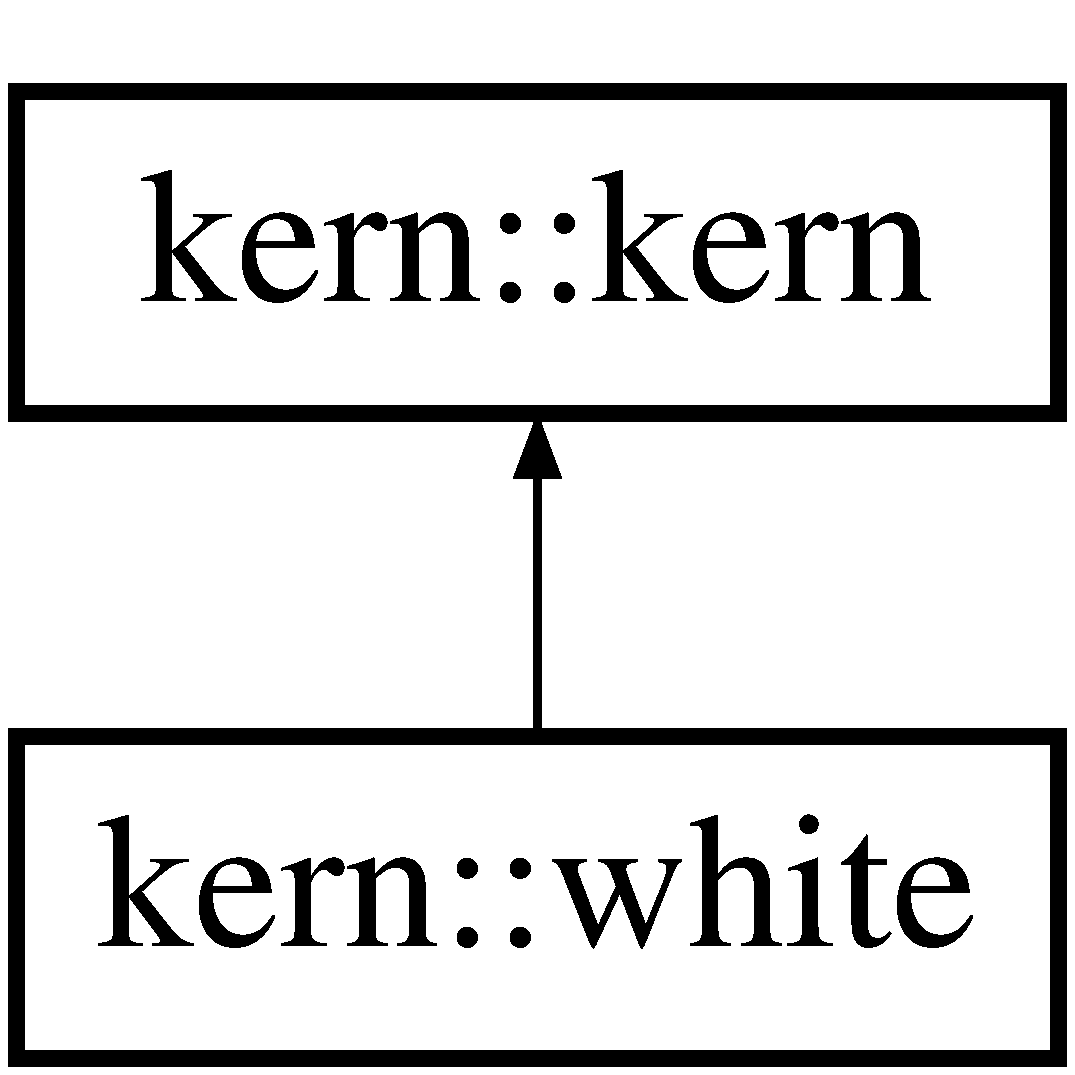
\includegraphics[height=2cm]{classkern_1_1white}
\end{center}
\end{figure}
\subsection*{Public Member Functions}
\begin{CompactItemize}
\item 
\hypertarget{classkern_1_1white_9a077edd7efcf16bee19b972a63965da}{
def \textbf{\_\-\_\-init\_\-\_\-}}
\label{classkern_1_1white_9a077edd7efcf16bee19b972a63965da}

\item 
def \hyperlink{classkern_1_1white_c9ce06fb072cdb4e1d769a8a926cc6fc}{paramInit}
\item 
def \hyperlink{classkern_1_1white_57249e12e16d1cda32db34818fc083ff}{compute}
\item 
def \hyperlink{classkern_1_1white_952f70cef3c05231022b3221d10d23ed}{diagCompute}
\item 
def \hyperlink{classkern_1_1white_1a7249a7d74e3282f581a4ac80be35ce}{diagGradX}
\item 
def \hyperlink{classkern_1_1white_3a2f74e8f49816b15e75b067e312f7dc}{diagGradient}
\item 
def \hyperlink{classkern_1_1white_ec5a23f33a26211bdfa4c8c5d0e022fe}{display}
\item 
def \hyperlink{classkern_1_1white_da7b491984621299ab25fef437d4b1b2}{expandParam}
\item 
def \hyperlink{classkern_1_1white_9b1bed2b896a0f9f15e3d568c2f2c54a}{extractParam}
\item 
\hypertarget{classkern_1_1white_7e5528f089942ba4b2899ae5bc2aff37}{
def \textbf{extractParamNames}}
\label{classkern_1_1white_7e5528f089942ba4b2899ae5bc2aff37}

\item 
def \hyperlink{classkern_1_1white_621f9c599dbfca7a038e9d5da8da8bc8}{gradX}
\item 
def \hyperlink{classkern_1_1white_e9f2b22e87fdf88c17187a3eb31f76a6}{gradient}
\end{CompactItemize}
\subsection*{Public Attributes}
\begin{CompactItemize}
\item 
\hypertarget{classkern_1_1white_f5cf170cd78074778ef09fbec4610dba}{
\textbf{type}}
\label{classkern_1_1white_f5cf170cd78074778ef09fbec4610dba}

\item 
\hypertarget{classkern_1_1white_ac4659d233f10f526e120db6ef20a71d}{
\textbf{variance}}
\label{classkern_1_1white_ac4659d233f10f526e120db6ef20a71d}

\item 
\hypertarget{classkern_1_1white_dfb12b863daec988bc9892398b76532a}{
\textbf{nParams}}
\label{classkern_1_1white_dfb12b863daec988bc9892398b76532a}

\item 
\hypertarget{classkern_1_1white_f595166954c01b9366b88839b4afe405}{
\textbf{stationary}}
\label{classkern_1_1white_f595166954c01b9366b88839b4afe405}

\end{CompactItemize}


\subsection{Detailed Description}


\footnotesize\begin{verbatim}% The white noise kernel arises from assuming independent Gaussian
% noise for each point in the function. The variance of the noise is
% given by the kern.variance parameter.
% 
% This kernel is not intended to be used independently, it is provided
% so that it may be combined with other kernels in a compound kernel.\end{verbatim}
\normalsize
 

\subsection{Member Function Documentation}
\hypertarget{classkern_1_1white_57249e12e16d1cda32db34818fc083ff}{
\index{kern::white@{kern::white}!compute@{compute}}
\index{compute@{compute}!kern::white@{kern::white}}
\subsubsection[{compute}]{\setlength{\rightskip}{0pt plus 5cm}def kern::white::compute ( {\em self}, \/   {\em x}, \/   {\em x2} = {\tt None})}}
\label{classkern_1_1white_57249e12e16d1cda32db34818fc083ff}




\footnotesize\begin{verbatim}% WHITEKERNCOMPUTE Compute the WHITE kernel given the parameters and X.
% FORMAT
% DESC computes the kernel parameters for the white noise
% kernel given inputs associated with rows and columns.
% ARG kern : the kernel structure for which the matrix is computed.
% ARG x : the input matrix associated with the rows of the kernel.
% ARG x2 : the inpute matrix associated with the columns of the kernel.
% RETURN k : the kernel matrix computed at the given points.
%
% FORMAT
% DESC computes the kernel matrix for the white noise
% kernel given a design matrix of inputs.
% ARG kern : the kernel structure for which the matrix is computed.
% ARG x : input data matrix in the form of a design matrix.
% RETURN k : the kernel matrix computed at the given points.
%
% SEEALSO : whiteKernParamInit, kernCompute, create, whiteKernDiagCompute
%
% COPYRIGHT : Neil D. Lawrence, 2004, 2005, 2006, 2009

\end{verbatim}
\normalsize
 

Reimplemented from \hyperlink{classkern_1_1kern}{kern::kern}.\hypertarget{classkern_1_1white_952f70cef3c05231022b3221d10d23ed}{
\index{kern::white@{kern::white}!diagCompute@{diagCompute}}
\index{diagCompute@{diagCompute}!kern::white@{kern::white}}
\subsubsection[{diagCompute}]{\setlength{\rightskip}{0pt plus 5cm}def kern::white::diagCompute ( {\em self}, \/   {\em x})}}
\label{classkern_1_1white_952f70cef3c05231022b3221d10d23ed}




\footnotesize\begin{verbatim}% WHITEKERNDIAGCOMPUTE Compute diagonal of WHITE kernel.
% FORMAT
% DESC computes the diagonal of the kernel matrix for the white noise kernel given a design matrix of inputs.
% ARG kern : the kernel structure for which the matrix is computed.
% ARG x : input data matrix in the form of a design matrix.
% RETURN k : a vector containing the diagonal of the kernel matrix
% computed at the given points.
%
% SEEALSO : whiteKernParamInit, kernDiagCompute, create, whiteKernCompute
%
% COPYRIGHT : Neil D. Lawrence, 2004, 2005, 2006, 2009

\end{verbatim}
\normalsize
 

Reimplemented from \hyperlink{classkern_1_1kern}{kern::kern}.\hypertarget{classkern_1_1white_3a2f74e8f49816b15e75b067e312f7dc}{
\index{kern::white@{kern::white}!diagGradient@{diagGradient}}
\index{diagGradient@{diagGradient}!kern::white@{kern::white}}
\subsubsection[{diagGradient}]{\setlength{\rightskip}{0pt plus 5cm}def kern::white::diagGradient ( {\em self}, \/   {\em X}, \/   {\em covDiag})}}
\label{classkern_1_1white_3a2f74e8f49816b15e75b067e312f7dc}




\footnotesize\begin{verbatim}% WHITEKERNDIAGGRADIENT Compute the gradient of the WHITE kernel's diagonal wrt parameters.
% FORMAT
% DESC computes the gradient of functions of the diagonal of the
% white noise kernel matrix with respect to the parameters of the kernel. The
% parameters' gradients are returned in the order given by the
% whiteKernExtractParam command.
% ARG kern : the kernel structure for which the gradients are
% computed.
% ARG x : the input data for which the gradient is being computed.
% ARG factors : partial derivatives of the function of interest with
% respect to the diagonal elements of the kernel.
% RETURN g : gradients of the relevant function with respect to each
% of the parameters. Ordering should match the ordering given in
% whiteKernExtractParam.
%
% SEEALSO : whiteKernParamInit, kernDiagGradient, whiteKernExtractParam, whiteKernGradient
%
% COPYRIGHT : Neil D. Lawrence, 2004, 2005, 2006, 2009

\end{verbatim}
\normalsize
 

Reimplemented from \hyperlink{classkern_1_1kern}{kern::kern}.\hypertarget{classkern_1_1white_1a7249a7d74e3282f581a4ac80be35ce}{
\index{kern::white@{kern::white}!diagGradX@{diagGradX}}
\index{diagGradX@{diagGradX}!kern::white@{kern::white}}
\subsubsection[{diagGradX}]{\setlength{\rightskip}{0pt plus 5cm}def kern::white::diagGradX ( {\em self}, \/   {\em X})}}
\label{classkern_1_1white_1a7249a7d74e3282f581a4ac80be35ce}




\footnotesize\begin{verbatim}% WHITEKERNDIAGGRADX Gradient of WHITE kernel's diagonal with respect to X.
% FORMAT
% DESC computes the gradient of the diagonal of the white noise kernel matrix with
% respect to the elements of the design matrix given in X.
% ARG kern : the kernel structure for which gradients are being computed.
% ARG X : the input data in the form of a design matrix.
% RETURN gX : the gradients of the diagonal with respect to each element
% of X. The returned matrix has the same dimensions as X.
%
% SEEALSO : whiteKernParamInit, kernDiagGradX, whitekernGradX
%
% COPYRIGHT : Neil D. Lawrence, 2004, 2005, 2006, 2009

\end{verbatim}
\normalsize
 

Reimplemented from \hyperlink{classkern_1_1kern}{kern::kern}.\hypertarget{classkern_1_1white_ec5a23f33a26211bdfa4c8c5d0e022fe}{
\index{kern::white@{kern::white}!display@{display}}
\index{display@{display}!kern::white@{kern::white}}
\subsubsection[{display}]{\setlength{\rightskip}{0pt plus 5cm}def kern::white::display ( {\em self}, \/   {\em numSpaces} = {\tt 0})}}
\label{classkern_1_1white_ec5a23f33a26211bdfa4c8c5d0e022fe}




\footnotesize\begin{verbatim}% WHITEKERNDISPLAY Display parameters of the WHITE kernel.
% FORMAT
% DESC displays the parameters of the white noise
% kernel and the kernel type to the console.
% ARG kern : the kernel to display.
%
% FORMAT does the same as above, but indents the display according
% to the amount specified.
% ARG kern : the kernel to display.
% ARG spacing : how many spaces to indent the display of the kernel by.
%
% SEEALSO : whiteKernParamInit, modelDisplay, kernDisplay
%
% COPYRIGHT : Neil D. Lawrence, 2004, 2005, 2006, 2009

\end{verbatim}
\normalsize
 

Reimplemented from \hyperlink{classkern_1_1kern}{kern::kern}.\hypertarget{classkern_1_1white_da7b491984621299ab25fef437d4b1b2}{
\index{kern::white@{kern::white}!expandParam@{expandParam}}
\index{expandParam@{expandParam}!kern::white@{kern::white}}
\subsubsection[{expandParam}]{\setlength{\rightskip}{0pt plus 5cm}def kern::white::expandParam ( {\em self}, \/   {\em params})}}
\label{classkern_1_1white_da7b491984621299ab25fef437d4b1b2}




\footnotesize\begin{verbatim}% WHITEKERNEXPANDPARAM Create kernel structure from WHITE kernel's parameters.
% FORMAT
% DESC returns a white noise kernel structure filled with the
% parameters in the given vector. This is used as a helper function to
% enable parameters to be optimised in, for example, the NETLAB
% optimisation functions.
% ARG kern : the kernel structure in which the parameters are to be
% placed.
% ARG param : vector of parameters which are to be placed in the
% kernel structure.
% RETURN kern : kernel structure with the given parameters in the
% relevant locations.
%
% SEEALSO : whiteKernParamInit, whiteKernExtractParam, kernExpandParam
%
% COPYRIGHT : Neil D. Lawrence, 2004, 2005, 2006

\end{verbatim}
\normalsize
 \hypertarget{classkern_1_1white_9b1bed2b896a0f9f15e3d568c2f2c54a}{
\index{kern::white@{kern::white}!extractParam@{extractParam}}
\index{extractParam@{extractParam}!kern::white@{kern::white}}
\subsubsection[{extractParam}]{\setlength{\rightskip}{0pt plus 5cm}def kern::white::extractParam ( {\em self})}}
\label{classkern_1_1white_9b1bed2b896a0f9f15e3d568c2f2c54a}




\footnotesize\begin{verbatim}% WHITEKERNEXTRACTPARAM Extract parameters from the WHITE kernel structure.
% FORMAT
% DESC Extract parameters from the white noise kernel structure into a
% vector of parameters for optimisation.
% ARG kern : the kernel structure containing the parameters to be
% extracted.
% RETURN param : vector of parameters extracted from the kernel. If
% the field 'transforms' is not empty in the kernel matrix, the
% parameters will be transformed before optimisation (for example
% positive only parameters could be logged before being returned).
%
% FORMAT
% DESC Extract parameters and parameter names from the white noise
% kernel structure.
% ARG kern : the kernel structure containing the parameters to be
% extracted.
% RETURN param : vector of parameters extracted from the kernel. If
% the field 'transforms' is not empty in the kernel matrix, the
% parameters will be transformed before optimisation (for example
% positive only parameters could be logged before being returned).
% RETURN names : cell array of strings giving paramter names.
%
% SEEALSO whiteKernParamInit, whiteKernExpandParam, kernExtractParam, scg, conjgrad
%
% COPYRIGHT : Neil D. Lawrence, 2004, 2005, 2006
%
\end{verbatim}
\normalsize
 \hypertarget{classkern_1_1white_e9f2b22e87fdf88c17187a3eb31f76a6}{
\index{kern::white@{kern::white}!gradient@{gradient}}
\index{gradient@{gradient}!kern::white@{kern::white}}
\subsubsection[{gradient}]{\setlength{\rightskip}{0pt plus 5cm}def kern::white::gradient ( {\em self}, \/   {\em X}, \/   {\em X2} = {\tt None}, \/   {\em covGrad} = {\tt None})}}
\label{classkern_1_1white_e9f2b22e87fdf88c17187a3eb31f76a6}




\footnotesize\begin{verbatim}% WHITEKERNGRADIENT Gradient of WHITE kernel's parameters.
% FORMAT
% DESC computes the gradient of functions with respect to the
% white noise
% kernel's parameters. As well as the kernel structure and the
% input positions, the user provides a matrix PARTIAL which gives
% the partial derivatives of the function with respect to the
% relevant elements of the kernel matrix. 
% ARG kern : the kernel structure for which the gradients are being
% computed.
% ARG x : the input locations for which the gradients are being
% computed. 
% ARG partial : matrix of partial derivatives of the function of
% interest with respect to the kernel matrix. The argument takes
% the form of a square matrix of dimension  numData, where numData is
% the number of rows in X.
% RETURN g : gradients of the function of interest with respect to
% the kernel parameters. The ordering of the vector should match
% that provided by the function kernExtractParam.
%
% FORMAT
% DESC computes the derivatives as above, but input locations are
% now provided in two matrices associated with rows and columns of
% the kernel matrix. 
% ARG kern : the kernel structure for which the gradients are being
% computed.
% ARG x1 : the input locations associated with the rows of the
% kernel matrix.
% ARG x2 : the input locations associated with the columns of the
% kernel matrix.
% ARG partial : matrix of partial derivatives of the function of
% interest with respect to the kernel matrix. The matrix should
% have the same number of rows as X1 and the same number of columns
% as X2 has rows.
% RETURN g : gradients of the function of interest with respect to
% the kernel parameters.
%
% SEEALSO whiteKernParamInit, kernGradient, whiteKernDiagGradient, kernGradX
%
% COPYRIGHT : Neil D. Lawrence, 2004, 2005, 2006, 2009

\end{verbatim}
\normalsize
 

Reimplemented from \hyperlink{classkern_1_1kern}{kern::kern}.\hypertarget{classkern_1_1white_621f9c599dbfca7a038e9d5da8da8bc8}{
\index{kern::white@{kern::white}!gradX@{gradX}}
\index{gradX@{gradX}!kern::white@{kern::white}}
\subsubsection[{gradX}]{\setlength{\rightskip}{0pt plus 5cm}def kern::white::gradX ( {\em self}, \/   {\em X}, \/   {\em X2} = {\tt None})}}
\label{classkern_1_1white_621f9c599dbfca7a038e9d5da8da8bc8}




\footnotesize\begin{verbatim}% WHITEKERNGRADX Gradient of WHITE kernel with respect to input locations.
% FORMAT
% DESC computes the gradident of the white noise
% kernel with respect to the input positions where both the row
% positions and column positions are provided separately.
% ARG kern : kernel structure for which gradients are being
% computed.
% ARG x1 : row locations against which gradients are being computed.
% ARG x2 : column locations against which gradients are being computed.
% RETURN g : the returned gradients. The gradients are returned in
% a matrix which is numData2 x numInputs x numData1. Where numData1 is
% the number of data points in X1, numData2 is the number of data
% points in X2 and numInputs is the number of input
% dimensions in X.
%
% SEEALSO whiteKernParamInit, kernGradX, whiteKernDiagGradX
%
% COPYRIGHT : Neil D. Lawrence, 2004, 2005, 2006

\end{verbatim}
\normalsize
 

Reimplemented from \hyperlink{classkern_1_1kern}{kern::kern}.\hypertarget{classkern_1_1white_c9ce06fb072cdb4e1d769a8a926cc6fc}{
\index{kern::white@{kern::white}!paramInit@{paramInit}}
\index{paramInit@{paramInit}!kern::white@{kern::white}}
\subsubsection[{paramInit}]{\setlength{\rightskip}{0pt plus 5cm}def kern::white::paramInit ( {\em self}, \/   {\em inDim} = {\tt None}, \/   {\em X} = {\tt None})}}
\label{classkern_1_1white_c9ce06fb072cdb4e1d769a8a926cc6fc}




\footnotesize\begin{verbatim}% WHITEKERNPARAMINIT WHITE kernel parameter initialisation.
%
% SEEALSO : cmpndKernParamInit
%
% FORMAT
% DESC initialises the white noise
%  kernel structure with some default parameters.
% ARG kern : the kernel structure which requires initialisation.
% RETURN kern : the kernel structure with the default parameters placed in.
%
% SEEALSO : create, kernParamInit
%
% COPYRIGHT : Neil D. Lawrence, 2004, 2005, 2006, 2009

\end{verbatim}
\normalsize
 

The documentation for this class was generated from the following file:\begin{CompactItemize}
\item 
kern.py\end{CompactItemize}

\hypertarget{classkerndox_1_1white}{
\section{kerndox::white Class Reference}
\label{classkerndox_1_1white}\index{kerndox::white@{kerndox::white}}
}
Inheritance diagram for kerndox::white::\begin{figure}[H]
\begin{center}
\leavevmode
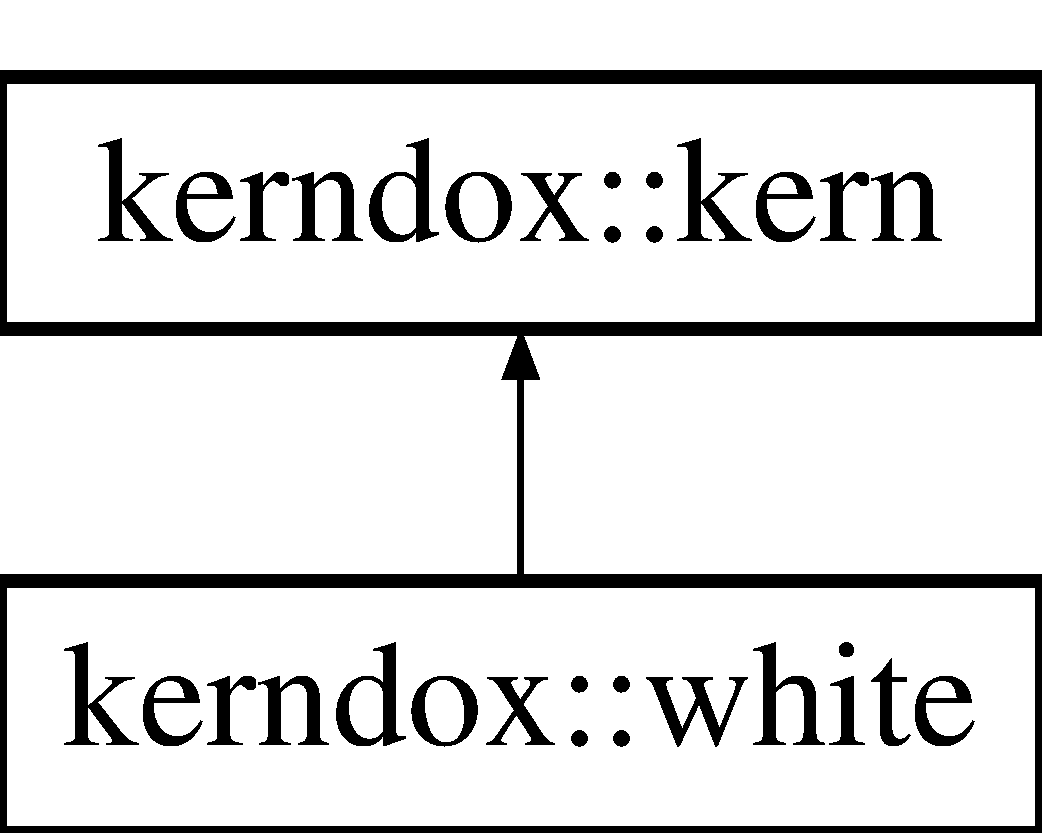
\includegraphics[height=2cm]{classkerndox_1_1white}
\end{center}
\end{figure}
\subsection*{Public Member Functions}
\begin{CompactItemize}
\item 
\hypertarget{classkerndox_1_1white_6962fe7a0c4cf91a9bdd44bedaf6bad9}{
def \textbf{\_\-\_\-init\_\-\_\-}}
\label{classkerndox_1_1white_6962fe7a0c4cf91a9bdd44bedaf6bad9}

\item 
def \hyperlink{classkerndox_1_1white_a20868e9e4488b9d80a70bf2e67b1438}{paramInit}
\item 
def \hyperlink{classkerndox_1_1white_805a650c553ae690536aa1000a2250e9}{compute}
\item 
def \hyperlink{classkerndox_1_1white_857c95585d0e30876382adacf58b52c2}{diagCompute}
\item 
def \hyperlink{classkerndox_1_1white_b0eee0d7ea27e278d7d39952053db3fc}{diagGradX}
\item 
def \hyperlink{classkerndox_1_1white_2f32c7f63de971d57148ab933073a791}{diagGradient}
\item 
def \hyperlink{classkerndox_1_1white_116d1d61e0eeee8609c876dba99a05d9}{display}
\item 
def \hyperlink{classkerndox_1_1white_ffc20aaa72aee2a83c2a57e70a67bce0}{expandParam}
\item 
def \hyperlink{classkerndox_1_1white_f4e9339bff592a00757fdd2f5bf6627a}{extractParam}
\item 
\hypertarget{classkerndox_1_1white_992a23fe6ed4b0600243ab4e0caa5a99}{
def \textbf{extractParamNames}}
\label{classkerndox_1_1white_992a23fe6ed4b0600243ab4e0caa5a99}

\item 
def \hyperlink{classkerndox_1_1white_b03d95c89f8e460fe5b1e8a97661e15c}{gradX}
\item 
def \hyperlink{classkerndox_1_1white_21428889944fc4070648f5d36f7c30a7}{gradient}
\end{CompactItemize}
\subsection*{Public Attributes}
\begin{CompactItemize}
\item 
\hypertarget{classkerndox_1_1white_d1f783449701904d62871311f470aaf5}{
\textbf{type}}
\label{classkerndox_1_1white_d1f783449701904d62871311f470aaf5}

\item 
\hypertarget{classkerndox_1_1white_29b711e2e7f9870fc34254399c2ad990}{
\textbf{variance}}
\label{classkerndox_1_1white_29b711e2e7f9870fc34254399c2ad990}

\item 
\hypertarget{classkerndox_1_1white_3636bb9a4884db30440b07aa34fa1c89}{
\textbf{nParams}}
\label{classkerndox_1_1white_3636bb9a4884db30440b07aa34fa1c89}

\item 
\hypertarget{classkerndox_1_1white_c4fdeddebe2980f0f87f4801eb0c777f}{
\textbf{stationary}}
\label{classkerndox_1_1white_c4fdeddebe2980f0f87f4801eb0c777f}

\end{CompactItemize}


\subsection{Detailed Description}


\footnotesize\begin{verbatim}The white noise kernel arises from assuming independent Gaussian
noise for each point in the function. The variance of the noise is
given by the kern.variance parameter.

This kernel is not intended to be used independently, it is provided
so that it may be combined with other kernels in a compound kernel.\end{verbatim}
\normalsize
 

\subsection{Member Function Documentation}
\hypertarget{classkerndox_1_1white_805a650c553ae690536aa1000a2250e9}{
\index{kerndox::white@{kerndox::white}!compute@{compute}}
\index{compute@{compute}!kerndox::white@{kerndox::white}}
\subsubsection[{compute}]{\setlength{\rightskip}{0pt plus 5cm}def kerndox::white::compute ( {\em self}, \/   {\em x}, \/   {\em x2} = {\tt None})}}
\label{classkerndox_1_1white_805a650c553ae690536aa1000a2250e9}




\footnotesize\begin{verbatim}WHITEKERNCOMPUTE Compute the WHITE kernel given the parameters and X.
FORMAT
DESC computes the kernel parameters for the white noise
kernel given inputs associated with rows and columns.
\param kern : the kernel structure for which the matrix is computed.
\param x : the input matrix associated with the rows of the kernel.
\param x2 : the inpute matrix associated with the columns of the kernel.
\return  k : the kernel matrix computed at the given points.
%
FORMAT
DESC computes the kernel matrix for the white noise
kernel given a design matrix of inputs.
\param kern : the kernel structure for which the matrix is computed.
\param x : input data matrix in the form of a design matrix.
\return  k : the kernel matrix computed at the given points.
%
SEEALSO : whiteKernParamInit, kernCompute, create, whiteKernDiagCompute
%
COPYRIGHT : Neil D. Lawrence, 2004, 2005, 2006, 2009

\end{verbatim}
\normalsize
 

Reimplemented from \hyperlink{classkerndox_1_1kern}{kerndox::kern}.\hypertarget{classkerndox_1_1white_857c95585d0e30876382adacf58b52c2}{
\index{kerndox::white@{kerndox::white}!diagCompute@{diagCompute}}
\index{diagCompute@{diagCompute}!kerndox::white@{kerndox::white}}
\subsubsection[{diagCompute}]{\setlength{\rightskip}{0pt plus 5cm}def kerndox::white::diagCompute ( {\em self}, \/   {\em x})}}
\label{classkerndox_1_1white_857c95585d0e30876382adacf58b52c2}




\footnotesize\begin{verbatim}WHITEKERNDIAGCOMPUTE Compute diagonal of WHITE kernel.
FORMAT
DESC computes the diagonal of the kernel matrix for the white noise kernel given a design matrix of inputs.
\param kern : the kernel structure for which the matrix is computed.
\param x : input data matrix in the form of a design matrix.
\return  k : a vector containing the diagonal of the kernel matrix
computed at the given points.
%
SEEALSO : whiteKernParamInit, kernDiagCompute, create, whiteKernCompute
%
COPYRIGHT : Neil D. Lawrence, 2004, 2005, 2006, 2009

\end{verbatim}
\normalsize
 

Reimplemented from \hyperlink{classkerndox_1_1kern}{kerndox::kern}.\hypertarget{classkerndox_1_1white_2f32c7f63de971d57148ab933073a791}{
\index{kerndox::white@{kerndox::white}!diagGradient@{diagGradient}}
\index{diagGradient@{diagGradient}!kerndox::white@{kerndox::white}}
\subsubsection[{diagGradient}]{\setlength{\rightskip}{0pt plus 5cm}def kerndox::white::diagGradient ( {\em self}, \/   {\em X}, \/   {\em covDiag})}}
\label{classkerndox_1_1white_2f32c7f63de971d57148ab933073a791}




\footnotesize\begin{verbatim}WHITEKERNDIAGGRADIENT Compute the gradient of the WHITE kernel's diagonal wrt parameters.
FORMAT
DESC computes the gradient of functions of the diagonal of the
white noise kernel matrix with respect to the parameters of the kernel. The
parameters' gradients are returned in the order given by the
whiteKernExtractParam command.
\param kern : the kernel structure for which the gradients are
computed.
\param x : the input data for which the gradient is being computed.
\param factors : partial derivatives of the function of interest with
respect to the diagonal elements of the kernel.
\return  g : gradients of the relevant function with respect to each
of the parameters. Ordering should match the ordering given in
whiteKernExtractParam.
%
SEEALSO : whiteKernParamInit, kernDiagGradient, whiteKernExtractParam, whiteKernGradient
%
COPYRIGHT : Neil D. Lawrence, 2004, 2005, 2006, 2009

\end{verbatim}
\normalsize
 

Reimplemented from \hyperlink{classkerndox_1_1kern}{kerndox::kern}.\hypertarget{classkerndox_1_1white_b0eee0d7ea27e278d7d39952053db3fc}{
\index{kerndox::white@{kerndox::white}!diagGradX@{diagGradX}}
\index{diagGradX@{diagGradX}!kerndox::white@{kerndox::white}}
\subsubsection[{diagGradX}]{\setlength{\rightskip}{0pt plus 5cm}def kerndox::white::diagGradX ( {\em self}, \/   {\em X})}}
\label{classkerndox_1_1white_b0eee0d7ea27e278d7d39952053db3fc}




\footnotesize\begin{verbatim}WHITEKERNDIAGGRADX Gradient of WHITE kernel's diagonal with respect to X.
FORMAT
DESC computes the gradient of the diagonal of the white noise kernel matrix with
respect to the elements of the design matrix given in X.
\param kern : the kernel structure for which gradients are being computed.
\param X : the input data in the form of a design matrix.
\return  gX : the gradients of the diagonal with respect to each element
of X. The returned matrix has the same dimensions as X.
%
SEEALSO : whiteKernParamInit, kernDiagGradX, whitekernGradX
%
COPYRIGHT : Neil D. Lawrence, 2004, 2005, 2006, 2009

\end{verbatim}
\normalsize
 

Reimplemented from \hyperlink{classkerndox_1_1kern}{kerndox::kern}.\hypertarget{classkerndox_1_1white_116d1d61e0eeee8609c876dba99a05d9}{
\index{kerndox::white@{kerndox::white}!display@{display}}
\index{display@{display}!kerndox::white@{kerndox::white}}
\subsubsection[{display}]{\setlength{\rightskip}{0pt plus 5cm}def kerndox::white::display ( {\em self}, \/   {\em numSpaces} = {\tt 0})}}
\label{classkerndox_1_1white_116d1d61e0eeee8609c876dba99a05d9}




\footnotesize\begin{verbatim}WHITEKERNDISPLAY Display parameters of the WHITE kernel.
FORMAT
DESC displays the parameters of the white noise
kernel and the kernel type to the console.
\param kern : the kernel to display.
%
FORMAT does the same as above, but indents the display according
to the amount specified.
\param kern : the kernel to display.
\param spacing : how many spaces to indent the display of the kernel by.
%
SEEALSO : whiteKernParamInit, modelDisplay, kernDisplay
%
COPYRIGHT : Neil D. Lawrence, 2004, 2005, 2006, 2009

\end{verbatim}
\normalsize
 

Reimplemented from \hyperlink{classkerndox_1_1kern}{kerndox::kern}.\hypertarget{classkerndox_1_1white_ffc20aaa72aee2a83c2a57e70a67bce0}{
\index{kerndox::white@{kerndox::white}!expandParam@{expandParam}}
\index{expandParam@{expandParam}!kerndox::white@{kerndox::white}}
\subsubsection[{expandParam}]{\setlength{\rightskip}{0pt plus 5cm}def kerndox::white::expandParam ( {\em self}, \/   {\em params})}}
\label{classkerndox_1_1white_ffc20aaa72aee2a83c2a57e70a67bce0}




\footnotesize\begin{verbatim}WHITEKERNEXPANDPARAM Create kernel structure from WHITE kernel's parameters.
FORMAT
DESC returns a white noise kernel structure filled with the
parameters in the given vector. This is used as a helper function to
enable parameters to be optimised in, for example, the NETLAB
optimisation functions.
\param kern : the kernel structure in which the parameters are to be
placed.
\param param : vector of parameters which are to be placed in the
kernel structure.
\return  kern : kernel structure with the given parameters in the
relevant locations.
%
SEEALSO : whiteKernParamInit, whiteKernExtractParam, kernExpandParam
%
COPYRIGHT : Neil D. Lawrence, 2004, 2005, 2006

\end{verbatim}
\normalsize
 \hypertarget{classkerndox_1_1white_f4e9339bff592a00757fdd2f5bf6627a}{
\index{kerndox::white@{kerndox::white}!extractParam@{extractParam}}
\index{extractParam@{extractParam}!kerndox::white@{kerndox::white}}
\subsubsection[{extractParam}]{\setlength{\rightskip}{0pt plus 5cm}def kerndox::white::extractParam ( {\em self})}}
\label{classkerndox_1_1white_f4e9339bff592a00757fdd2f5bf6627a}




\footnotesize\begin{verbatim}WHITEKERNEXTRACTPARAM Extract parameters from the WHITE kernel structure.
FORMAT
DESC Extract parameters from the white noise kernel structure into a
vector of parameters for optimisation.
\param kern : the kernel structure containing the parameters to be
extracted.
\return  param : vector of parameters extracted from the kernel. If
the field 'transforms' is not empty in the kernel matrix, the
parameters will be transformed before optimisation (for example
positive only parameters could be logged before being returned).
%
FORMAT
DESC Extract parameters and parameter names from the white noise
kernel structure.
\param kern : the kernel structure containing the parameters to be
extracted.
\return  param : vector of parameters extracted from the kernel. If
the field 'transforms' is not empty in the kernel matrix, the
parameters will be transformed before optimisation (for example
positive only parameters could be logged before being returned).
\return  names : cell array of strings giving paramter names.
%
SEEALSO whiteKernParamInit, whiteKernExpandParam, kernExtractParam, scg, conjgrad
%
COPYRIGHT : Neil D. Lawrence, 2004, 2005, 2006
%
\end{verbatim}
\normalsize
 \hypertarget{classkerndox_1_1white_21428889944fc4070648f5d36f7c30a7}{
\index{kerndox::white@{kerndox::white}!gradient@{gradient}}
\index{gradient@{gradient}!kerndox::white@{kerndox::white}}
\subsubsection[{gradient}]{\setlength{\rightskip}{0pt plus 5cm}def kerndox::white::gradient ( {\em self}, \/   {\em X}, \/   {\em X2} = {\tt None}, \/   {\em covGrad} = {\tt None})}}
\label{classkerndox_1_1white_21428889944fc4070648f5d36f7c30a7}




\footnotesize\begin{verbatim}WHITEKERNGRADIENT Gradient of WHITE kernel's parameters.
FORMAT
DESC computes the gradient of functions with respect to the
white noise
kernel's parameters. As well as the kernel structure and the
input positions, the user provides a matrix PARTIAL which gives
the partial derivatives of the function with respect to the
relevant elements of the kernel matrix. 
\param kern : the kernel structure for which the gradients are being
computed.
\param x : the input locations for which the gradients are being
computed. 
\param partial : matrix of partial derivatives of the function of
interest with respect to the kernel matrix. The argument takes
the form of a square matrix of dimension  numData, where numData is
the number of rows in X.
\return  g : gradients of the function of interest with respect to
the kernel parameters. The ordering of the vector should match
that provided by the function kernExtractParam.
%
FORMAT
DESC computes the derivatives as above, but input locations are
now provided in two matrices associated with rows and columns of
the kernel matrix. 
\param kern : the kernel structure for which the gradients are being
computed.
\param x1 : the input locations associated with the rows of the
kernel matrix.
\param x2 : the input locations associated with the columns of the
kernel matrix.
\param partial : matrix of partial derivatives of the function of
interest with respect to the kernel matrix. The matrix should
have the same number of rows as X1 and the same number of columns
as X2 has rows.
\return  g : gradients of the function of interest with respect to
the kernel parameters.
%
SEEALSO whiteKernParamInit, kernGradient, whiteKernDiagGradient, kernGradX
%
COPYRIGHT : Neil D. Lawrence, 2004, 2005, 2006, 2009

\end{verbatim}
\normalsize
 

Reimplemented from \hyperlink{classkerndox_1_1kern}{kerndox::kern}.\hypertarget{classkerndox_1_1white_b03d95c89f8e460fe5b1e8a97661e15c}{
\index{kerndox::white@{kerndox::white}!gradX@{gradX}}
\index{gradX@{gradX}!kerndox::white@{kerndox::white}}
\subsubsection[{gradX}]{\setlength{\rightskip}{0pt plus 5cm}def kerndox::white::gradX ( {\em self}, \/   {\em X}, \/   {\em X2} = {\tt None})}}
\label{classkerndox_1_1white_b03d95c89f8e460fe5b1e8a97661e15c}




\footnotesize\begin{verbatim}WHITEKERNGRADX Gradient of WHITE kernel with respect to input locations.
FORMAT
DESC computes the gradident of the white noise
kernel with respect to the input positions where both the row
positions and column positions are provided separately.
\param kern : kernel structure for which gradients are being
computed.
\param x1 : row locations against which gradients are being computed.
\param x2 : column locations against which gradients are being computed.
\return  g : the returned gradients. The gradients are returned in
a matrix which is numData2 x numInputs x numData1. Where numData1 is
the number of data points in X1, numData2 is the number of data
points in X2 and numInputs is the number of input
dimensions in X.
%
SEEALSO whiteKernParamInit, kernGradX, whiteKernDiagGradX
%
COPYRIGHT : Neil D. Lawrence, 2004, 2005, 2006

\end{verbatim}
\normalsize
 

Reimplemented from \hyperlink{classkerndox_1_1kern}{kerndox::kern}.\hypertarget{classkerndox_1_1white_a20868e9e4488b9d80a70bf2e67b1438}{
\index{kerndox::white@{kerndox::white}!paramInit@{paramInit}}
\index{paramInit@{paramInit}!kerndox::white@{kerndox::white}}
\subsubsection[{paramInit}]{\setlength{\rightskip}{0pt plus 5cm}def kerndox::white::paramInit ( {\em self}, \/   {\em inDim} = {\tt None}, \/   {\em X} = {\tt None})}}
\label{classkerndox_1_1white_a20868e9e4488b9d80a70bf2e67b1438}




\footnotesize\begin{verbatim}WHITEKERNPARAMINIT WHITE kernel parameter initialisation.
%
SEEALSO : cmpndKernParamInit
%
FORMAT
DESC initialises the white noise
 kernel structure with some default parameters.
\param kern : the kernel structure which requires initialisation.
\return  kern : the kernel structure with the default parameters placed in.
%
SEEALSO : create, kernParamInit
%
COPYRIGHT : Neil D. Lawrence, 2004, 2005, 2006, 2009

\end{verbatim}
\normalsize
 

The documentation for this class was generated from the following file:\begin{CompactItemize}
\item 
kerndox.py\end{CompactItemize}

\printindex
\end{document}
